%%%%% Ms. Vijaya Yaduvanshi(ME E&TC) 
%In this template sample content is entered. Kindly type/ Copy your own content and you can modify this as per your requirement.
%%%%%%%%%%%%%%%%%%%%%%%%%%%%%% 


\documentclass[12pt,a4paper]{report}
\fontfamily{times_new_roman}
\selectfont
\usepackage{amsmath}    
\usepackage{graphicx}
\usepackage[colorlinks=true,linkcolor=red]{hyperref}%%%%%%
\usepackage[left=1in,right=1in,top=1in,bottom=1in]{geometry}% to set margins
\usepackage{subfigure}
\usepackage{setspace}
\doublespacing
\spacing{1}
\usepackage{float}

%--------------------------------------------------------------------------------------------------------------------------------------------------------------------------------------------------------------------


\begin{document}
%\renewcommand{\baselinestretch}{1.15}
\begin{titlepage}

\begin{center}

\large{\bf{A}\\
\bf{Project Phase II Report}\\
on}\\

\vspace*{0.2in}

\textbf{\Large{COMPUTER VISION BASED COTTON HARVESTING ROVER}}

\vspace*{0.2in}

\large{SUBMITTED TO THE SAVITRIBAI PHULE PUNE UNIVERSITY,  PUNE}
\end{center}

%%%%****SSPU Logo****
\begin{figure}[!htb]

\begin{center}


\includegraphics[scale=1.0]{images/logo/logo.png}

\end{center}
\end{figure}

\begin{center}

\large{{IN THE PARTIAL FULFILMENT OF PROJECT PART-II OF THE REQUIREMENT FOR THE AWARD OF THE DEGREE}\\{OF}\\ \textbf{BACHELOR OF ELECTRONICS \& TELECOMMUNICATION ENGINEERING}\\ {BY}}
\end{center}
%%%%****%%%%
\begin{center}
 
 Abhimanyu Rajesh Kanase
  \hspace*{0.2in} Seat No. B191223027
\\
 Anshu Biju Varghese
 \hspace*{0.5in} Seat No. B191223062
\\
 Aditya Prasad Deshmukh   
 \hspace*{0.3in} Seat No. B191223017
\\
Under the guidance of \\
\vspace*{0.1in}
\textbf{\large{Prof.Dr.Rahul.G.Mapari}}

%%%****SSPU Logo****
\begin{figure}[!htb]
\begin{center}

\includegraphics[scale=1.0]{images/logo/pccoelogo.png}
\end{center}
\end{figure}
%%%%****%%%%

\large{Department of Electronics and Telecommunication
Engineering}\\

\Large{Pimpri Chinchwad College of Engineering and Research,Ravet,\\
Pune-412101\\

ACADEMIC YEAR:2023-24}
\end{center}

\end{titlepage}


%----------------------------------------------------------------------
%%% -------------------------Certificate Page-------------------------------------------------------------------------------------------------


\begin{center}
\bf{PIMPRI CHINCHWAD EDUCATION TRUST'S\\
Pimpri Chinchwad College of Engineering and Research,\\ Pune-412101}\\
\end{center}
\vspace*{0.3in}
\begin{figure}[!htb]
\begin{center}

\includegraphics[scale=1.0]{images/logo/pccoelogo.png}
\end{center}
\end{figure}
\begin{center}
{\huge \textbf{CERTIFICATE}}\\
\vspace*{0.3in}

This is to certify that the Project Phase-II report entitled \\
\vspace*{0.1in}
{\bf{``COMPUTER VISION BASED COTTON HARVESTING ROVER"}},\\
\vspace*{0.1in}
Submitted by \\
\vspace*{0.1in}
\bf{
Abhimanyu Rajesh Kanase \hspace*{0.2in} (Exam Seat No. B191223027)\\
Anshu Biju Varghese\hspace*{0.5in} (Exam Seat No. B191223062)\\
Aditya Prasad Deshmukh  \hspace*{0.3in} (Exam Seat No. B191223017)}\\
\end{center}


\vskip 0.2in
\noindent
is a bona fide work carried out by them under the supervision of {\bf{Prof.Dr.Rahul.G.Mapari}} and it is approved for the partial fulfillment of the Project Phase II of the
requirement of Savitribai Phule Pune University, Pune for the award of the degree of
Bachelor of Engineering (Electronics \& Telecommunication). The Dissertation work has
not been submitted to any other institute or university for the award of a degree.




\vskip 0.4in
\noindent
Prof.Kishor Bhangale \hspace{6cm} 
Prof.Dr.Rahul G.Mapari \hspace{1.9cm} \newline
\indent
{\bf{Project Guide}} \hspace{6 cm}
{\bf{Prof.Guide Name
}}\hspace{1.9cm}
 \hspace{0.10in}
 
\vskip 0.4in
\noindent
Prof.Dr.Rahul G.Mapari \hspace{6cm} 
Prof.Dr.H.U.Tiwari \hspace{1.9cm} \newline
\indent
{\bf{Head of Department} \hspace{6 cm}
\bf{Principal}}\hspace{1.9cm}
 \hspace{0.10in}



%--------------------------------------------------------------------------------------------------------------------------------------------------------------------------------------------------------------------




%%Acknowledgement

\chapter*{Acknowledgement\markboth{Acknowledgement}{Acknowledgement}}
\noindent

We are greatly indebted to Head of Electronics \& Telecommunication Engineering
and Project Guide {\bf{Prof.Dr.Rahul.G.Mapari}} for his able guidance throughout
the course  of this work.It has been anal together different experience to work
with him and we would like to thank him for his help,suggestions and numerous
discussions.
\\
\par We are heartily thankful to {\bf{ Prof.Dr.Harish U.Tiwari}} (Principal, Pimpri Chinchwad College of Engineering \& Research,Ravet)for providing research environment;also for his kind inspiration.
\\
\par We are gladly taking this opportunity to thank the Head of Electronics \& Telecommunication Engineering {\bf{Prof. Dr.Rahul Mapari}} and project Coordinator {\bf{Mr. Kishor Bhangale}} for their valuable guidance and providing facility during the progress of the seminar.
\\
\par
Last but not least we are also thankful to all those who help directly or indirectly to develop this Project work and complete it successfully. With Deep Reverence,
\vspace*{0.5in}


\begin{flushright}

\textbf{Abhimanyu Rajesh Kanase\\
        Anshu Biju Varghese\\
        Aditya Prasad Deshmukh}
\end{flushright}

\noindent
Date: \\
Place:


\tableofcontents
\listoffigures
\listoftables


%-------------------------------------------------------------------------------------------------------Abstract-----------------------------------------------------------------------------------------------------

%abstract
\begin{abstract}
%%Type abstract here instead of below content
\doublespacing
\par Cotton harvesting has historically required a lot of labor, taken a long time, and presented many difficulties. Yield and quality were inconsistent when harvested by hand. In traditional systems, the cotton blooms could not be detected accurately due to obstruction due to leaves, or detecting the sky instead of the cotton based on features like color, etc. In traditional harvesting, there were major concerns which included the preparation for plantation, determining the harvest season, manual labor, unavailability of skilled workers, and transport capability.
\par To deal with this matter the robotic technology used by Cotton Harvesting Rover is capable of identifying cotton blossoms precisely with the aid of computer vision technology. The cotton is automatically identified by the system as it selects flowers from the fields using a robotic arm after analyzing specific attributes.
\par The novelty of this project is that it identifies the cotton blooms from all perspectives so that inaccuracy can be avoided. With the help of the rover, it becomes convenient to keep plucking the mature cotton blooms and detecting them simultaneously. This solution helps reduce the labor work, increasing yield and quality and reducing of usage of harmful chemicals. 
\par The expected outcome of this idea is that the model should identify the mature cotton blooms accurately and the robotic arm should pick the cotton without much delay thus ensuring improved cotton harvesting.By increasing the effectiveness and sustainability of cotton harvesting, this ground-breaking approach has the potential to completely change the cotton business. The successful completion of this project is expected to produce a considerable improvement in cotton harvesting techniques by accurately identifying mature cotton blooms and enabling the robotic arm to function flawlessly.
\end{abstract}


%----------------------------------------------------------------------
%------------------------------------chapter1--------------------------
%----------------------------------------------------------------------


%%%CHAPTER 1
\chapter{Introduction}
\hspace{6pt}
\setstretch{1.5}
\par This chapter emphasizes the critical need for improving cotton harvesting methods and introduces an engineering project focused on developing a cotton-picking rover equipped with computer vision technology. It provides a detailed research background, defines the problem statement, outlines the project objectives, delineates the scope, and presents an overview of the proposed rover system.
%\large{Paragraph 1 of introduction . }

%--------------------------------Introduction--------------------------

\section{Introduction}
\par Traditionally cotton picking was done by using methodologies such as hand picking, chemical defoliation, mechanical stripping, manual picking machines, etc. The idea of the project is to develop an advanced cotton-picking robot that incorporates computer vision to enhance and upgrade the efficiency and accuracy of cotton harvesting. 
\par Computer vision is a field that allows computers to extract information from images and other visual inputs. Based on this information it takes necessary actions. It trains the machines to perform according to the functionality that is indicated to be done. Computer vision can be used in various applications such as the detection of faces, video capturing, and tracking moving objects. Using image processing and computer vision the cotton bolls can be detected based on their features and the robotic arm aims to pick them and store them in a container. A deep learning object detection model called YOLOv5 (You Only Look Once version 5) is employed for cotton blossom detection in real-time. The process for successful cotton boll detection includes data collection, labeling the data, selecting the version of the model, training the model by providing the annotated dataset, fine-tuning, and then evaluating the results based on test datasets. Finally, the model is integrated into the robotic system for real-time cotton boll collection.
\par The rover’s functionality will be to move autonomously through the cotton fields. The system will be equipped with cameras and image processing capabilities to analyze each cotton bloom particularly and identify the ripe ones.


%--------------------------research backgrond--------------------------


\section {Research background}
\par Prior to starting a project that entails using robotics and computer vision to build a cotton-picking rover, extensive research covering several crucial topics was done:
\begin{enumerate}
   \item {\bf{ Cotton Plant Biology :}} \cite{r5}\cite{r4}Acquired knowledge of the characteristics, stages, and growth cycles of cotton plants. To find cotton, research was done to understand its visual characteristics at various growth stages.
   \item {\bf{ Optimal Picking Techniques:}} Explored the most efficient methods for cotton harvesting that won't damage the plants or lower output.
\end{enumerate}
{\bf{ Automation and Robotics:}}  
\begin{enumerate}
   \item {\bf{ Robotic Arm Capabilities:}} \cite{r13} Analyzed the accuracy of current robotic arm designs and their applicability to precise tasks like cotton picking.
   \item {\bf{ Mobile Robotics:}}  Investigated rover designs, propulsion systems, and techniques for traversing diverse terrains.
\end{enumerate}
{\bf{ Computer vision and image processing:}}
\begin{enumerate}
   \item {\bf{ Algorithms:}} \cite{r9}\cite{r10}Used OpenCV to research various methods of object recognition and detection, including CNNs, Haar cascades, and contour detection for plant recognition.
  \item {\bf{ Image processing techniques:}} \cite{r3}Inquired about color thresholding, feature extraction, and other image processing techniques to distinguish cotton plants from the background.
\end{enumerate}



% ---------------------------Problem statement-------------------------


\section {Problem Statement}
\par To develop a cotton harvesting rover using computer vision which identifies and
selectively picks up mature cotton blooms from the plants, hence reducing labor
dependencies and improves crop yield.

%-----------------------------Objective--------------------------------

\section{Objectives of the Study}
\par The objectives of the proposed works are mentioned as follows
\begin{enumerate}
    \item To develop an image processing model that accurately identifies cotton bolls among other plants.
   \item To ensure that plucked cotton bolls are not damaged.
   \item To minimize the total initial cost for the system
   \item To ensure that hardware setup and software model are well integrated.
   \item To distinguish mature cotton blooms from pre-matured ones
   \item To make certain that the system is portable, robust, and has increased mobility.
   \item To make sure that repair and maintenance are easy and cost-efficient. 
\end{enumerate}


%------------------------------scope---------------------------------


\section {Scope of the Study}
\par A project that builds a cotton-picking rover with computer vision and robotics has a wide scope and touches on a number of different fields:
\par Technical Features: Creating and assembling the rover's robotic arm, cameras, sensors, and motors while ensuring proper hardware integration is known as hardware integration.
\par Software Engineering: Write code for object detection, image processing, and identification using computer vision. Creating algorithms to control the robotic arm and identify cotton plants against a backdrop is required for this.
\par Developing the navigation and control systems that will enable the rover to go through fields, avoid obstructions, and reach the designated cotton plants.
%\par Real-time Performance: Quick and efficient cotton harvesting is made possible by real-time data processing.Iteration and testing: To ensure accuracy


%--------------------overview of proposed system-----------------------


\section {Overview of Proposed System}

\par    Description of the proposed system and overall block diagram are as follows:
\\
\par The proposed system uses cameras in cotton fields to record color, shape, and size images. In order to distinguish between mature and premature cotton blossoms, computer vision analyzes these photos using a Convolutional Neural Network (CNN). When ripe cotton bolls are identified, a robotic arm is triggered to gather and store them in a container. The CNN is trained using labeled datasets. The rover's ability to navigate the field with efficiency is its main goal.\\


\begin{figure}[!htb]
\begin{center}
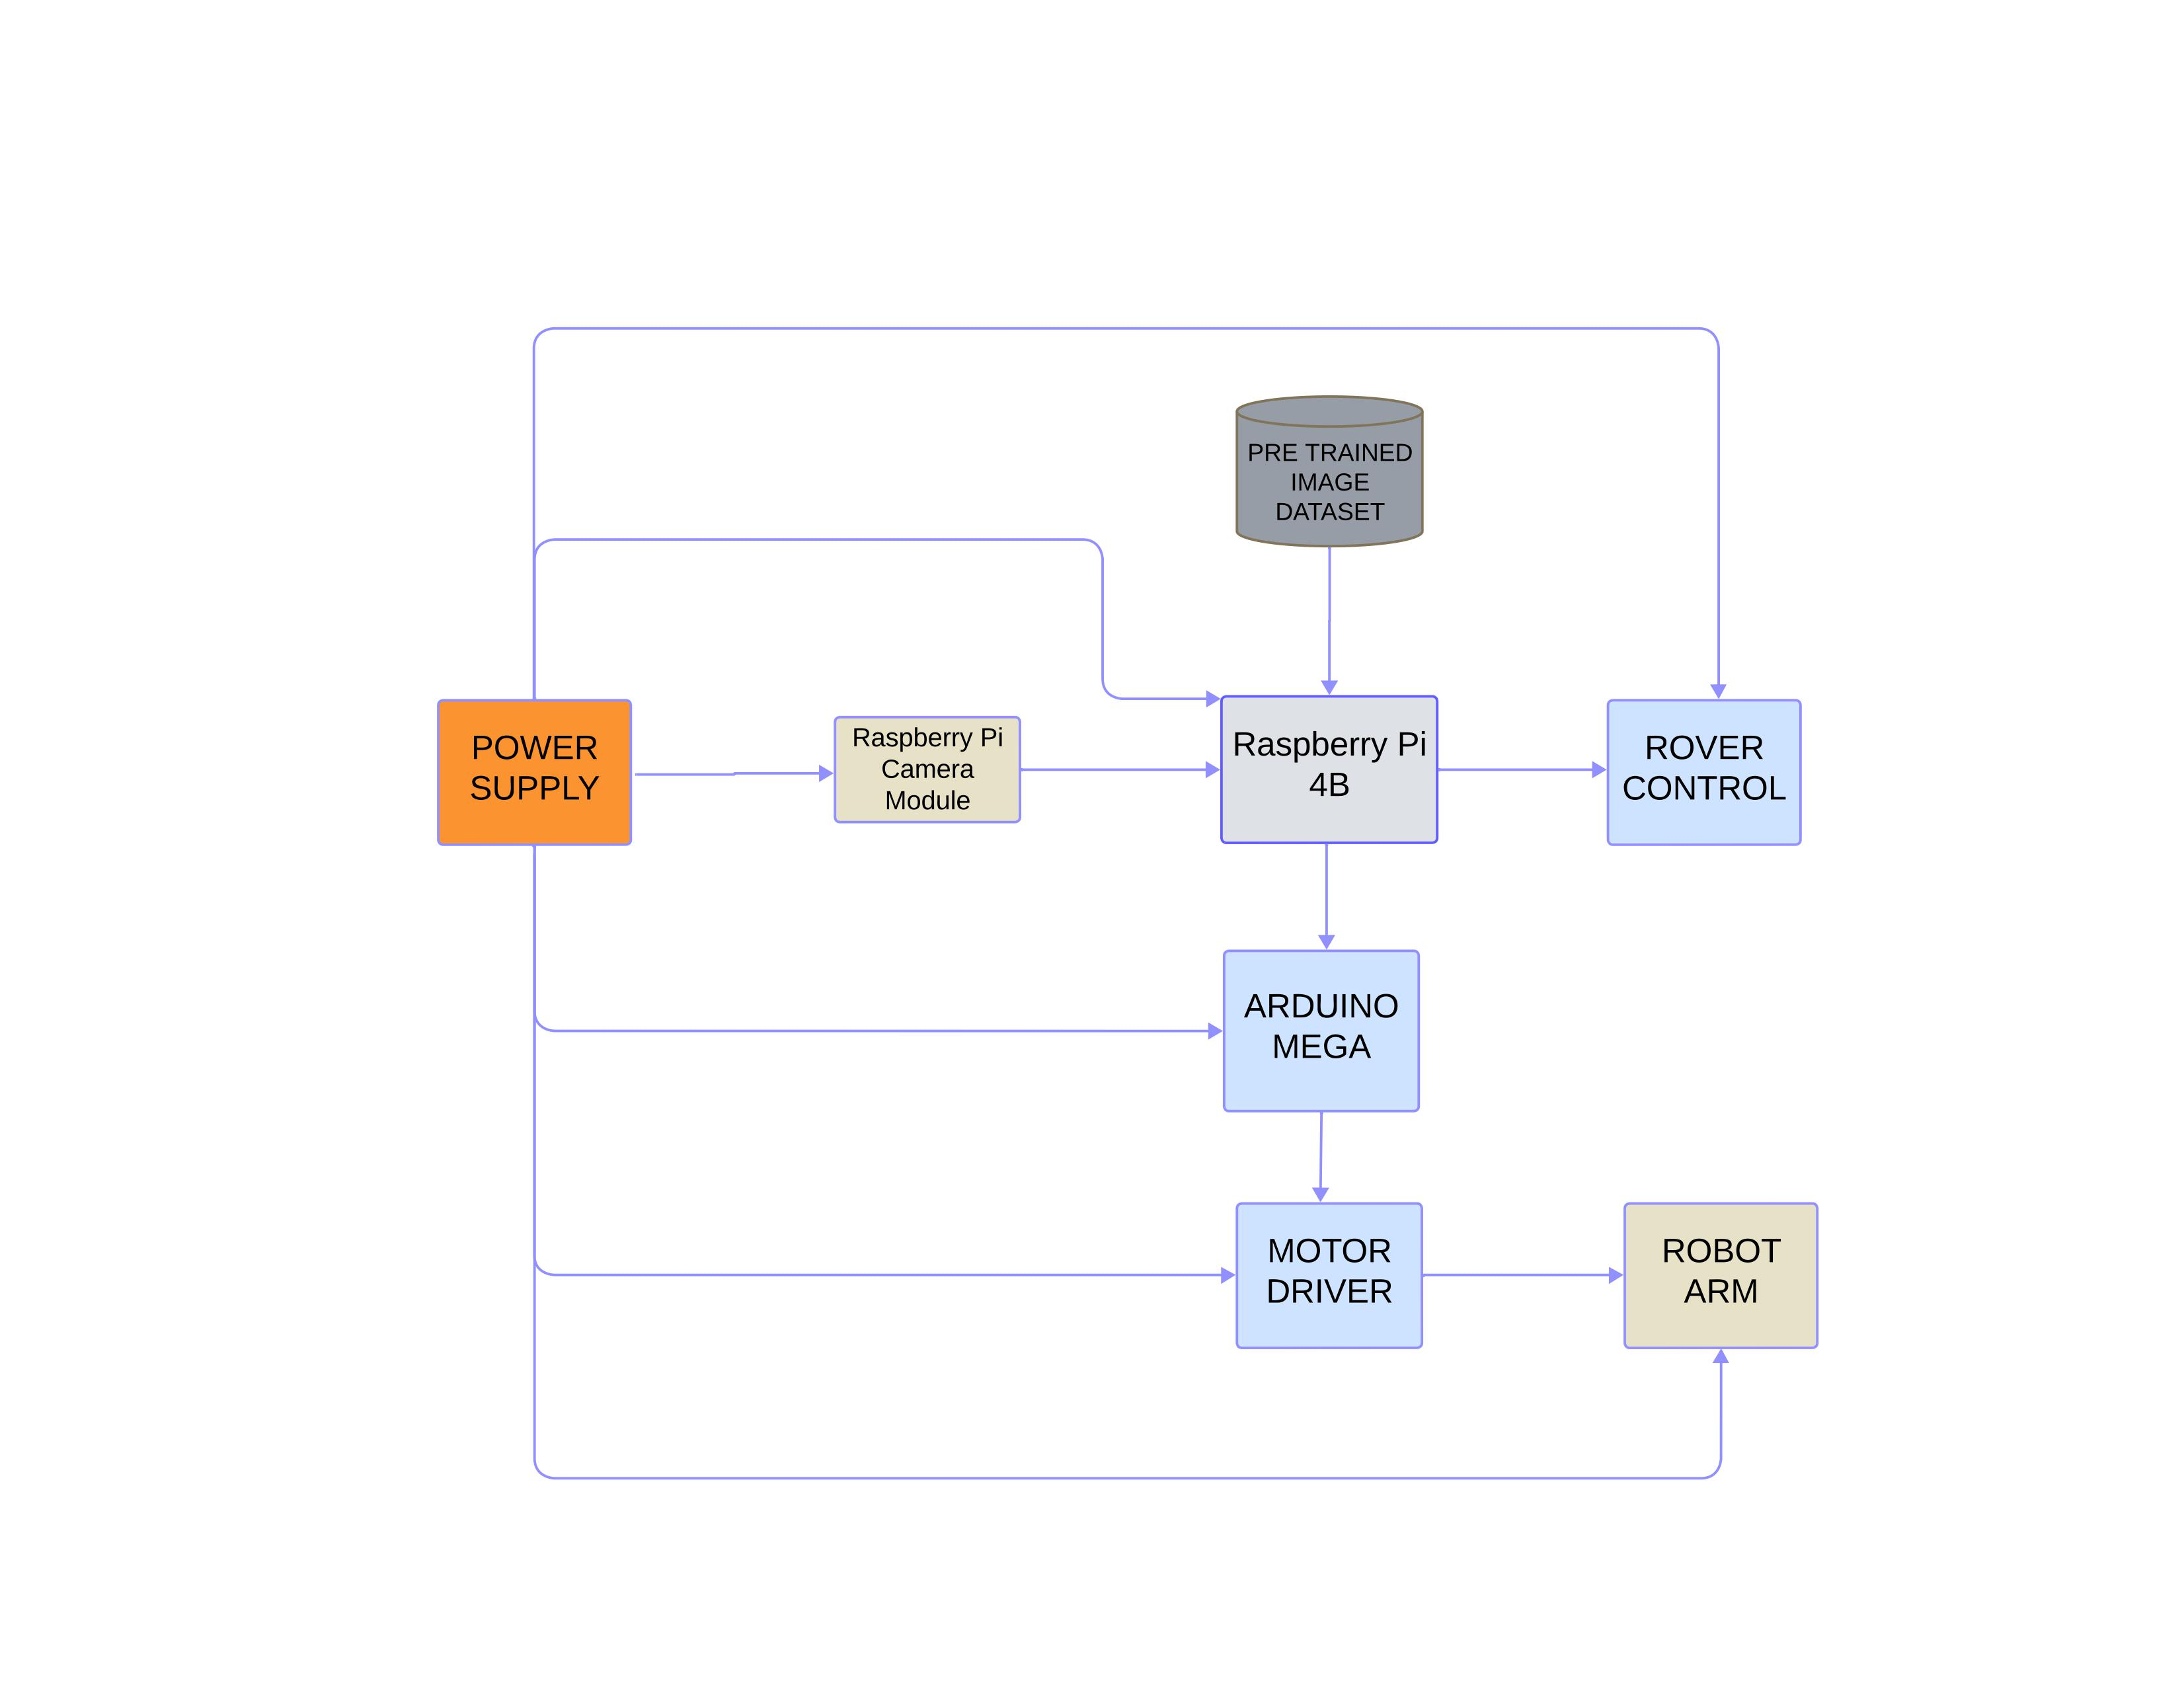
\includegraphics[scale=0.5]{images/diagrams/blockdig.jpg}
\caption{Block Diagram}
\end{center}
\end{figure}




%------------------------organization of report------------------------%


\section {Organization of the Report}


\par The project report is organized as follows:
\\* Chapter 1 Introduction: Provides the information regarding the introduction of ..area, need, relevance, problem statement, objectives, and scope of the study. Further, it provides a short overview of the proposed system.
\\
Chapter 2 Literature Review: Gives a survey of various articles on the used technology and provides the major gaps that pave the way for the development of the proposed system.
\\
Chapter 3 Proposed Methodology: Provides the system implementation, data pre-processing, information about YOLOv5, designn , objectives completed till date and  flowchart.
\\
Chapter 4 Results and Discussions: Gives an overview of hardware setup, software setup, and results.  
\\
Chapter 5 Advantages and Applications: Provides the advantages and applications of the project. 
\\
Chapter 6: Conclusion and Future Scope: Consists of the conclusion and future scope of the project.
\\
Chapter 7: Consists of the references used.

%----------------------------------------------------------------------
%----------------------------chapter2----------------------------------
%----------------------------------------------------------------------


%CHAPT 2
\chapter{Literature Review}



%-------------------------Literature survey---------------------------


 
\section {Literature Survey}


\par A promising method for harvesting cotton in India and other developing nations is Cotton Harvesters. Even though there have been significant advancements in recent years, there are still difficulties with its implementation in India. All cotton picking in developed nations is done by machines. The Indian agriculture sector has become more mechanized due to rising labor costs and a shortage of labor \cite{r1}. According to Haolu Li, remote sensing imageries were used for accurate identification of cotton crop. The deep-learning model used was DenseNet, which is a multidimensional densely connected convolutional network. Remote sensing techniques benefit viewpoints like growth monitoring, disease identification, area estimation and multiple parameters. SVM can do agricultural classification in which the support vectors are limited and the training dataset can be reduced without altering the accuracy of classification. Remote sensing images are obtained from satellites, unmanned air vehicles (UAVs) and unmanned ground vehicles (UGV) \cite{r2}. Xu et al detail the procedure for gathering aerial photos of cotton fields, analyzing the photos to determine possible bloom locations, and employing a convolutional neural network to categorize the possible blooms as either non-blooming objects or cotton flowers.[4]Deep Learning based models like RCNN perform better than ML algorithms like multi-layer perceptron and K-nearest neighbour to achieve a high detection rate. ResNet-18 was more accurate than Random Forest (70.16 \%) and Support Vector Machine (60.6 \%) \cite{r3}.
\par K. Fue  describes, the utilization of OpenCV (version 3.3.0) mission vision to detect cotton and Robot Operating System (ROS) for rover and robot arm control. Z. Xu et al have explained cotton detection using fuzzy reasoning-based approach combined with RGB and HSV color spaces to manipulate image color pixel values and set upper/lower limits for white cotton bolls. Amanda Issac et al \cite{r6}. This paper concludes that they were able to achieve a joint reduction in dimensionality and file size by combining the bitwise-masking and PCA processes on sliced images. This technique produced a significant percentage of smaller files while preserving high-quality reconstructions, outperforming the default JPEG compression \cite{r7}. Adalberto I. S. Oliveira developed a robot whose purpose is to monitor the cotton crop and move between rows of crops. The control system of the robot consists of an image-based visual servoing method and a fuzzy logic-based controller \cite{r8}. The potential to enhance cotton farming techniques through automation and robotics, from pre-planting to harvesting and ginning. The authors contend that utilizing technology to enhance cotton farming methods has a wide range of possible advantages. Utilizing programs such as OpenCV, ROS, PBI Logger Utility, a John Deere program, and the plastic-inspection-detection-ejection system (PIDES) \cite{r9}. According to Zhang, Yan and Yang etc an Improved YOLOv5 network was presented that integrated DenseNet, attention mechanism, and bi-frequency frequency prediction to correctly and economically identify unopened cotton bolls in the field. According to the experiment results, the suggested approach outperforms the original YOLOv5 model as well as alternative approaches like YOLOv3, SSD, and FasterRCNN when taking into account the simultaneous considerations of detection accuracy, computational cost, model size, and speed \cite{r10}.
\par Yong Wang and the research team present a novel approach to cotton recognition based on color subtraction information of various cotton components. Besides, dynamic Freeman chain coding is used to reduce noise and improve recognition accuracy in order to raise the accuracy rate of cotton recognition \cite{r11}. Nimkar Amey Sanjay concludes that to create sustainable and successful agriculture, the goal of the project is to identify, harvest, and store cotton using a cotton harvester that makes use of strong digital analytics, robotics, and image processing. The machine would pluck several crops by using multiple robotic arms built in the harvest zone \cite{r12}. This machine is ideal for women because it is remote-controlled and electrically operated, eliminating the need for a driver. This work by W. M. Porter explores and validates the optical detection of cotton rows. The row depth is detected using a stereo camera, and the upper and lower portions of the cotton row canopy are then calculated using a pixel-based method that assumes a normal distribution for the high and low pixels. Pixel-based sliding window algorithms and perspective transform are used to detect left and right rows. For the cotton-picking robot to navigate smoothly, the center of the rows is calculated along with the Bayesian score of the detection \cite{r13}. According to Kadeghe Fue SMACH, a ROS-independent library for finite state machines, is utilized by the system. Using a 2D manipulator that travels linearly in both the horizontal and vertical directions, the robot harvests the bolls. The finite state machine's decision directs the manipulator and the rover to the destination, and the stereo camera parameters are used to calculate the boll 3-D location. To regulate the rover's journey to the boll, PID control is used \cite{r14}. This work by Spyros Fountas is an overview of the existing research on scientific agricultural robotic systems and their uses in weeding, crop monitoring, phenotyping, disease detection, spraying, navigation, and harvesting is covered in this work. The review also covers the many kinds of AI algorithms and sensors that are employed in these systems \cite{r15}. 
\par This paper focuses on the development of an improved YOLOv5 algorithm for the detection of appearance-based damage in cotton seeds \cite{r16}. The creation of a computer vision algorithm that uses YOLOv5m to identify volunteer cotton plants in cornfields is covered in the document\cite{r17}. This paper used Point annotation and multi-scale fusion-based cotton boll localization approach \cite{r19}. It details the construction and deviation analysis of an image processing-based 5-axis robotic arm. The study offers an affordable technique for doing laboratory tests on a robotic arm \cite{r20}. The report provides a comprehensive overview of the latest advancements in LiDAR technology and its potential applications in ground crop analysis \cite{r23}.The X, Y, and Z axes deviations are provided in the paper. Image processing carried out in MATLAB was used to calculate them. The deviation is detected to be roughly 0.3 mm in the X, 0.1 to 0.2 mm in the Y, and 0.1 mm in the Z axes \cite{r21}. The creation of an instructional robotic arm with color detection and object handling capabilities is suggested in this research using a vision-based control system. There are possible uses for the system in education, employment, and training \cite{r22} . An overview of sensors and systems in navigation systems, recognition and detection algorithm classification, and crop row techniques are given in this work \cite{r24}.



%--------------------------finding LS----------------------------------%



\section {Findings from Literature Survey}
\par From the widespread survey of various techniques of Cotton Picking using deep learning we found the following gaps that needed to be concentrated.


% \\ 
% \begin{table}
% \begin{center}
\subsection {Gap Identification} % title of Table
\par According to the existing literature and the state of knowledge in object detection, there are some limitations that may arise in the methodology, observed findings and some questions which may be unanswered. The below table contains all the gaps/limitations which were identified during the analysis of the papers. This paper describes the existing methodology, the design and formulation, methods for data collection and their drawbacks. Based on this analysis it is possible to address issues that had been faced in the previous research papers. 
       Around 26 papers were studied, out of which 25 gaps were 
identified.
     The gap identification from the following papers
are as follows:
The cost and availability of labor are two major issues that Indian cotton farmers must deal with \cite{r1}. Machine learning techniques do not use automatic feature extraction and need careful tuning of hyperparameters \cite{r4}. In real field obstruction caused by branches and other leaves can result in longer picking time. Implementation cost due to hardware, software, and maintenance is high \cite{r5}. Detects only white cotton bolls therefore may not be directly applicable to other types of crops or monitoring scenarios. Requires specialized equipment \cite{r6}. Specifies the outlines the application case for identifying flowering patterns in cotton blooms, and does not specify other use cases. Does not specify the computational requirement and time complexity \cite{r7}. Potential challenges faced can be field obstacles, theft, cost, etc. Due to the system being autonomous, they must require minimal management time \cite{r9}. Techniques like YOLOv3, SSD, and Faster-RCNN showed less performance in terms of detection, computational costing, model size, and speed \cite{r10}. Requires specific lighting conditions, does not work well with certain types of cotton \cite{r11}. This paper focuses on the development of a cotton harvester using ML and IP techniques and not on the practical use \cite{r12}. New automated machines will have to match the reliability, self-sufficiency, and economic competitiveness of the existing harvesters used in the U.S \cite{r13}. The system was struggling to get a boll if it is located behind the stem or branch. Some-times it causes the system to leave behind some bolls \cite{r14}. Need for specialized sensors and algorithm calibration, difficulty in comparing AI algorithm performances among papers using different data sets \cite{r15}. It is deficient in thorough assessment, comparative analysis, and specific details on a few key areas, including the computational efficiency and the algorithm's performance with coated cotton seeds \cite{r16}. ACO algorithm used for generating the optimal path and spot-spray is stochastic in nature and may not provide a globally optimal solution \cite{r17}. Not all of the computational resources needed for MCBLNet training and implementation, particularly in real-time applications may have been taken into consideration \cite{r19}. Testing equipment for robotic arms is costly \cite{r20}. Challenges involved in complexity in robotic arm programming \cite{r21}. Possible drawbacks could be limited to only color and shape recognition, environmental conditions could impact the reliability of computer vision \cite{r22}. The challenges of differentiating between crop species, the requirement for extreme precision and accuracy in data collection, and the possibility of interference from meteorological elements like wind and rain \cite{r23}. Accurate direction-finding and self-governing agricultural equipment are challenged by the unstructured and complicated character of the agricultural environment \cite{r24}.


\subsection {{\bf{ From the literature survey following gaps are identified :}}} 
 
\begin{enumerate}
    \item Obstruction caused due to leaves, branches or other materials can slow the picking time.
    \item Implementation cost due to hardware, software, and maintenance.
    \item Autonomous systems must have less maintenance time.
    \item Only identifies specific cotton blooming patterns and does not specify other use cases. 
    \item Could not identify cotton bolls which were hidden behind some branches leaving behind some bolls. 
\end{enumerate}







%-----------------------------------------------------------------------------------------------------chapter 3------------------------------------------------------------------------------------------------------

%CHAPT 3


\chapter{Proposed Methodology }





\section {System Implementation/Block Diagram and Explanation}
 
\begin{figure}[!htb]
\begin{center}
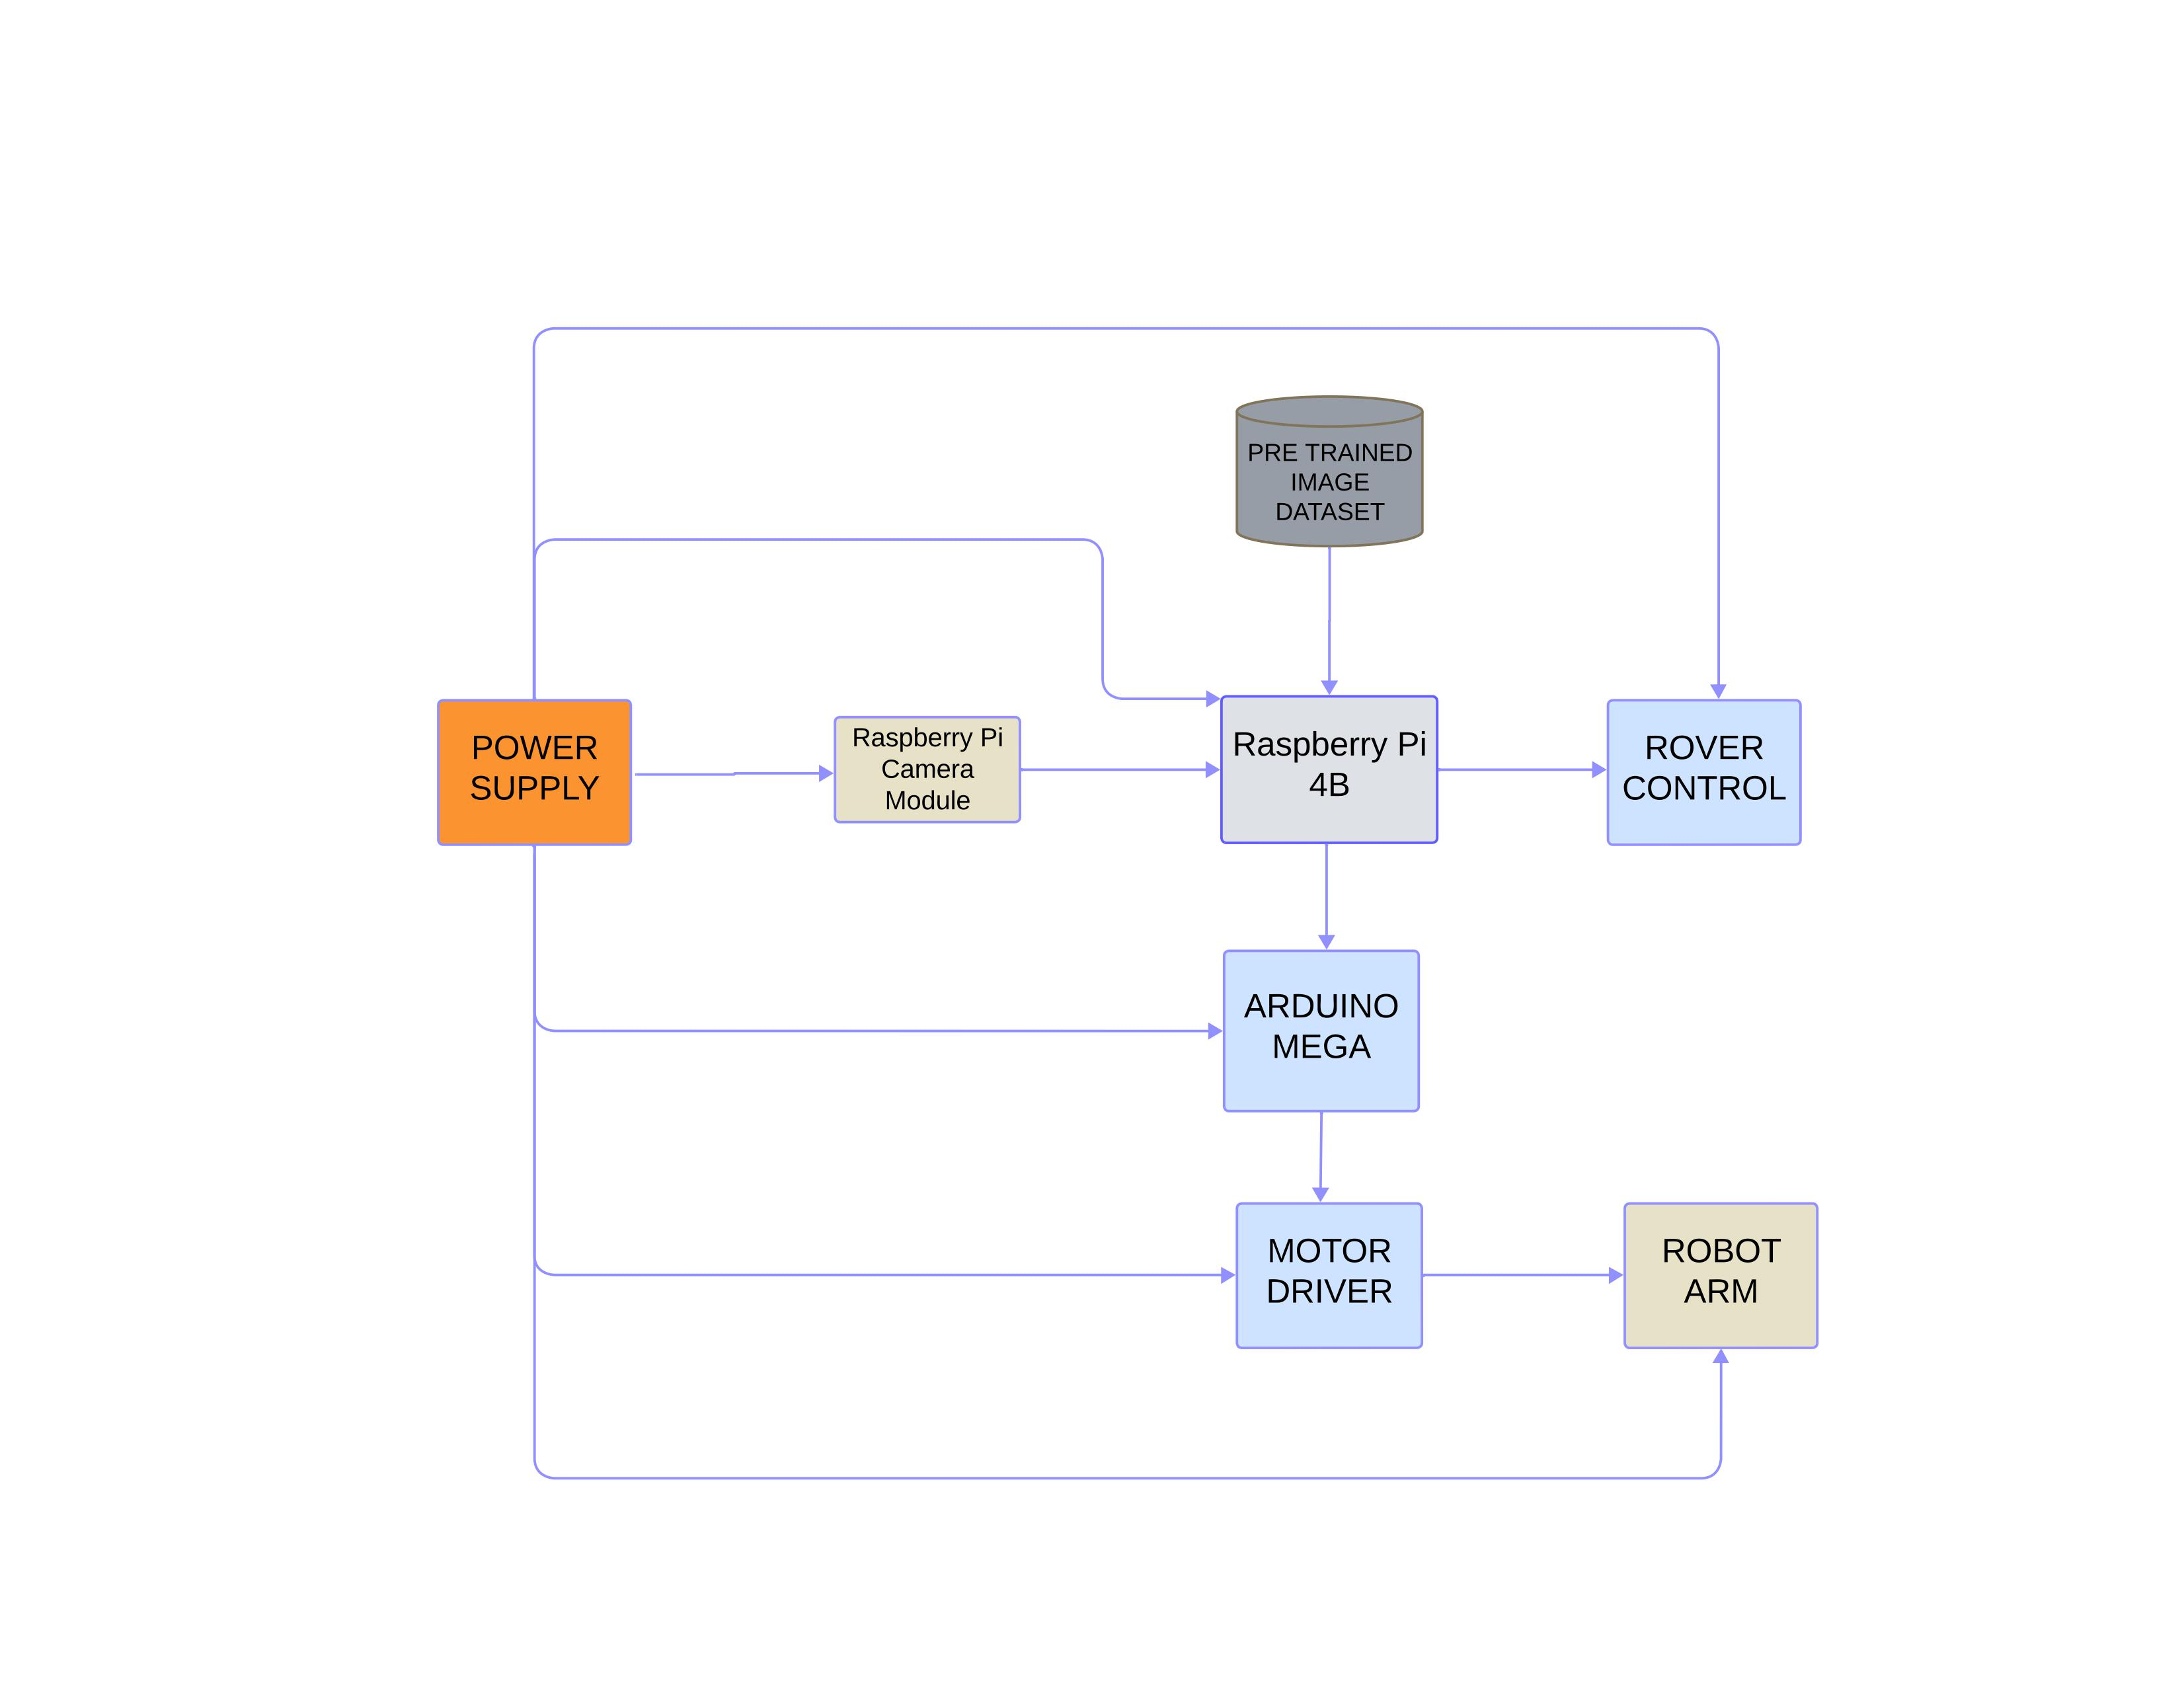
\includegraphics[scale=0.5]{images/diagrams/blockdig.jpg}
\caption{Block Diagram}
\end{center}
\end{figure}
\newpage
\par A trained model called YOLO v5 for cotton detection is shown in the above block diagram. It is capable of recognizing cotton bolls from their surroundings. 1421 distinct annotated images using Roboflow were used to train the model on Google Collab plus platform. The trained model could be deployed on Raspberry Pi to carry out the cotton detection using the robotic arm. This model in future will be integrated with the robotic arm. The Raspberry Pi initiates the model's operation by receiving a video feed from the Raspberry Cam. The trained model then processes the video and sends the user the detected cotton boll. The cotton is then harvested from the plant by feeding the robot arm having 6 DOF with the coordinates that the system has determined for the cotton boll's location.

%\newpage



\section {Data preprocessing}
\par The Dataset was collected from two different websites, Roboflow. We utilized every bit of data from the over 1421 photos in the Roboflow dataset.In order to precisely represent the many stages and components of the cotton plant, the dataset is divided into five classes: split cotton boll, matured cotton boll, early boll, cotton blossom, and cotton bud. The process of creating the model was facilitated by the pre-labeled and annotated internet dataset that we gathered. 
\begin{figure}[!htb]
\begin{center}
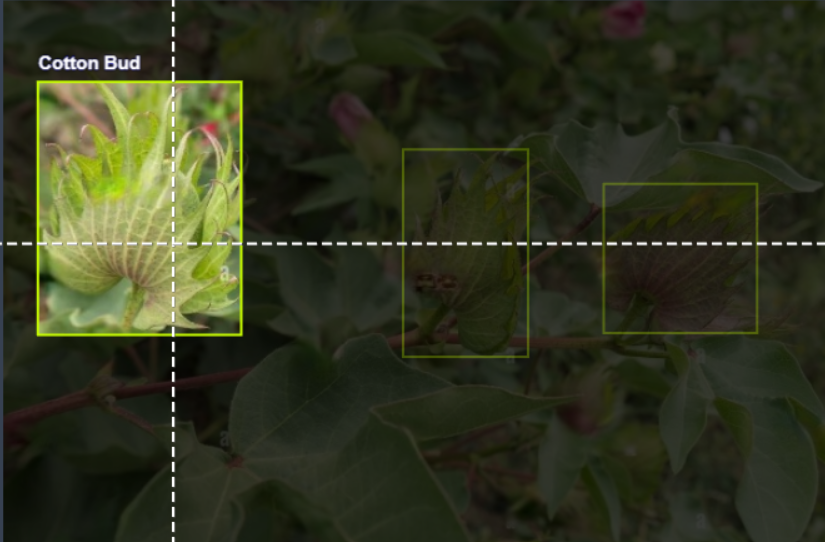
\includegraphics[scale=0.4]{images/detection/bud.png}
\caption{Detection of cotton bud}
\end{center}
\end{figure}
\begin{figure}[!htb]
\begin{center}
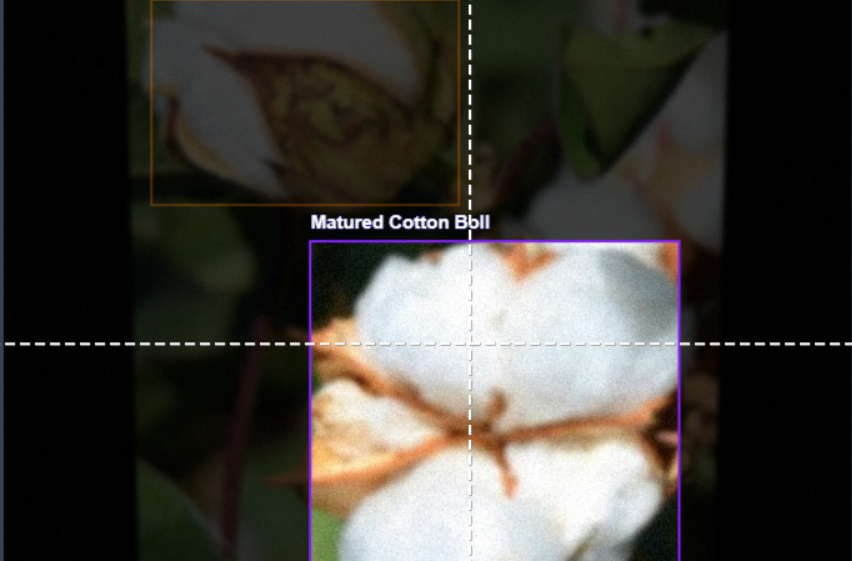
\includegraphics[scale=0.4]{images/detection/matured.png}
\caption{Detection of matured cotton boll}
\end{center}
\end{figure}
\par The images were preprocessed, followed by data augmentation, resizing. Before preprocessing, the dataset's image resolution was 640x640 pixels. 85\% of the data set is used for training, 10\% is used for validation, and 5\% is used for testing \cite{r27}. The dataset contains images of individual cotton bolls on the plant to help the model recognize cotton bolls up close, and images of multiple cotton bolls on a single plant to help the model detect cotton bolls at a distance.
\par Data preprocessing converts raw data into a format that computers and machine learning can comprehend and analyze as part of the data analysis process. In this process auto-orientation and resizing of the images is done. Auto-orientation adjusts the and corrects the orientation to make sure image are aligned properly. The images are then resized to 640x640 , which means that the original aspect ratio of images is changed. We annotated the photographs by putting an anchor box around the area of interest that has to be detected to obtain raw data for our investigation. The cotton boll in this case is growing in several stages, including split, maturity, early, and flower. By first specifying all classes for each growth stage and then selecting a particular class each time a bounding box is created during the annotation process, this can be split into five categories. The next stage is data augmentation after each image has been annotated. In augmentation for an original image , 3 augmented versions have been generated. During this procedure, the photographs are rotated 90 degrees in both clockwise and counterclockwise directions, flipped vertically and horizontally, and their exposure is adjusted between -12\% and +12\% to increase the size of the data. The Roboflow platform was used for data augmentation and annotation, and the dataset was exported in a format compatible with PyTorch version 5 \cite{r27}. 







\section {Detection using Yolov5}
\par \hspace*{0.2in}This paper describes how YOLOv5, a deep learning-based pre-trained model, can be explicitly trained for a cotton dataset and, once installed, be able to recognize cotton in any surroundings. The specific goals at hand and the availability of data for the model's training are the determining factors when choosing YOLOv5 or any other machine-learning model. To achieve high-performance object identification, YOLO models are used. YOLO divides an image into grid systems, and each grid system is aware of its contents.

\begin{table}[H]
\begin{center}
\caption{Comparison of YOLO versions}% title of Table
\hspace*{0.2in} 
\\
\begin{tabular}{| p{3cm} | p{4cm} | p{4cm} | p{2cm} |}
\hline
{\bf{Parameter}}             &{\bf{YOLOv4}} & {\bf{YOLOv5}}             &{\bf{YOLOv7}}  \\ \hline
Speed& Varies based on the model selected & Has good balance & Fastest \\ \hline
Accuracy & Varies according   to the selected mode &	Offers good balance &	Highest\\ \hline
Open- source &	No &	Yes	& No \\ \hline
Training data	& COCO
dataset &	Diverse D5 dataset &	COCO
dataset
\\ \hline
Computation power &	Higher generally	& Low than v4	& Lowest \\ \hline
\end{tabular}
\end{center}
\end{table}


In the above table, various YOLO versions are compared. Since v5 is open source, lighter than v7, and more accurate than v4, it is the most appropriate of them for our application in cotton detection. Version 5 uses a variety of D5 datasets for data training, whereas versions 4 and 7 only use the COCO dataset, as shown in the table below. The cotton detection research uses this model:
\begin{figure}[H]
\begin{center}
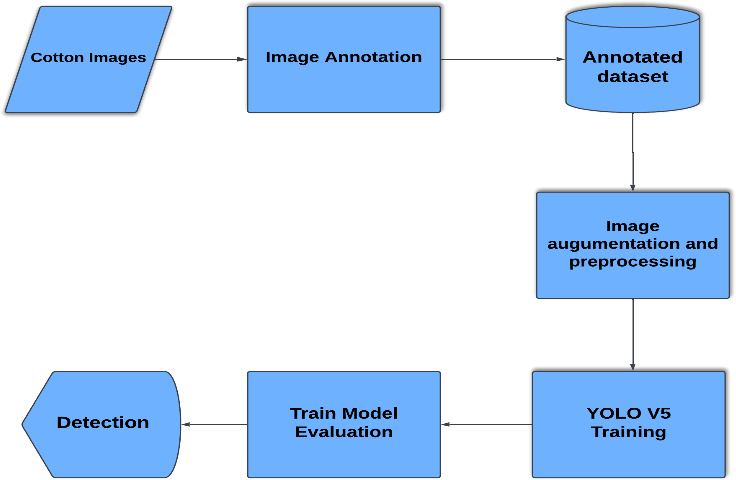
\includegraphics[scale=0.65]{images/methodology/Generalized_flow_of_YOLOv5_cotton_detection_model.png}
\caption{Generalized flow of YOLOv5 cotton detection model}
\end{center}
\end{figure}
\par The explanation of the YOLO cotton detecting model is provided in above figure:
\par {\bf{Cotton Image}}: The initial stage of model training is data collection. This information was obtained from several sources, including cotton grown in a greenhouse or a laboratory, among others. The Roboflow dataset is used for training.
\par {\bf{Image Annotation}}: Machine learning and artificial intelligence techniques are used to annotate images. Often, image annotation is carried out by human annotators who use an image annotation tool to label photos or tag pertinent information, such as assigning the proper classifications to different objects in an image. We created two classes for our model, as mentioned in the section on picture datasets. For simple tasks like classification and segmentation, pre-trained models are usually available. These models can be tailored to specific use cases with the help of Transfer Learning and little data. The comprehensive description of the Roboflow platform, where the annotation was finished, may be found in the data preprocessing section.
\par {\bf{Annotated Dataset}}: The data is sent to the Colab for model training after going through the platform's annotation process. It is separated into three sections: test, validation, and training. 
\par {\bf{Image augmentation and preprocessing}}: Before exporting the dataset to Colab, it is first made larger using the augmentation technique, which is covered in detail in the data pretreatment section.
\par {\bf{YOLOv5 training}}: To train our v5 model on our custom dataset, we first export our previously processed data from the Roboflow platform in a format that is compatible with Python. After everything is finished, a repository code is produced. We set the parameters to start training after importing the dataset into Colab using the code. Initially, we adjusted the image size to match the export size. The epochs for this model are then set. To train our model, we tried training it with epochs ranging from 50 to 200; however, the best results were obtained with a batch size of 32 and 150 epochs. We obtained an accuracy of 0.83 by using this input value. 
\par {\bf{Train Model Evaluation}}: We use the trained model to perform object detection in test set photos after testing it on unseen data. After an object has been detected, the performance is evaluated, and metrics including precision, mAP, and the accuracy and effectiveness of the model in object detection are examined.  
\par {\bf{Detection}}: After cotton is detected, a box enclosing the cotton emerges, which appears to represent the degree of confidence. This level only expresses the degree of confidence that the object being recognized is cotton or not (for instance, a level of 0.8 would indicate an 80\% confidence level on cotton detection).
%\newpage

\begin{table}[H]
\begin{center}
\caption{Configuration details of Yolo}% title of Table
\hspace*{0.2in}
\\
\begin{tabular}{| p{5cm} | p{5cm} |}
\hline
{\bf{Parameter}}             &{\bf{Details}}          \\ \hline
Batch Size	& 32 \\ \hline
Model	& YOLOv5s\\ \hline
Loss function	& Returns class loss, box loss, object loss\\ \hline
Convolutional network& Backbone-Darknet \\ &Neck-PANet 
\\ \hline
Epochs &	150\\ \hline
Resolution &	640 x 640\\ \hline
Activation function &	SiLU and Sigmoid activation function\\ \hline
\end{tabular}
\end{center}
\end{table} 






\section {Yolov5 architecture}
\begin{figure}[!htb]
\begin{center}
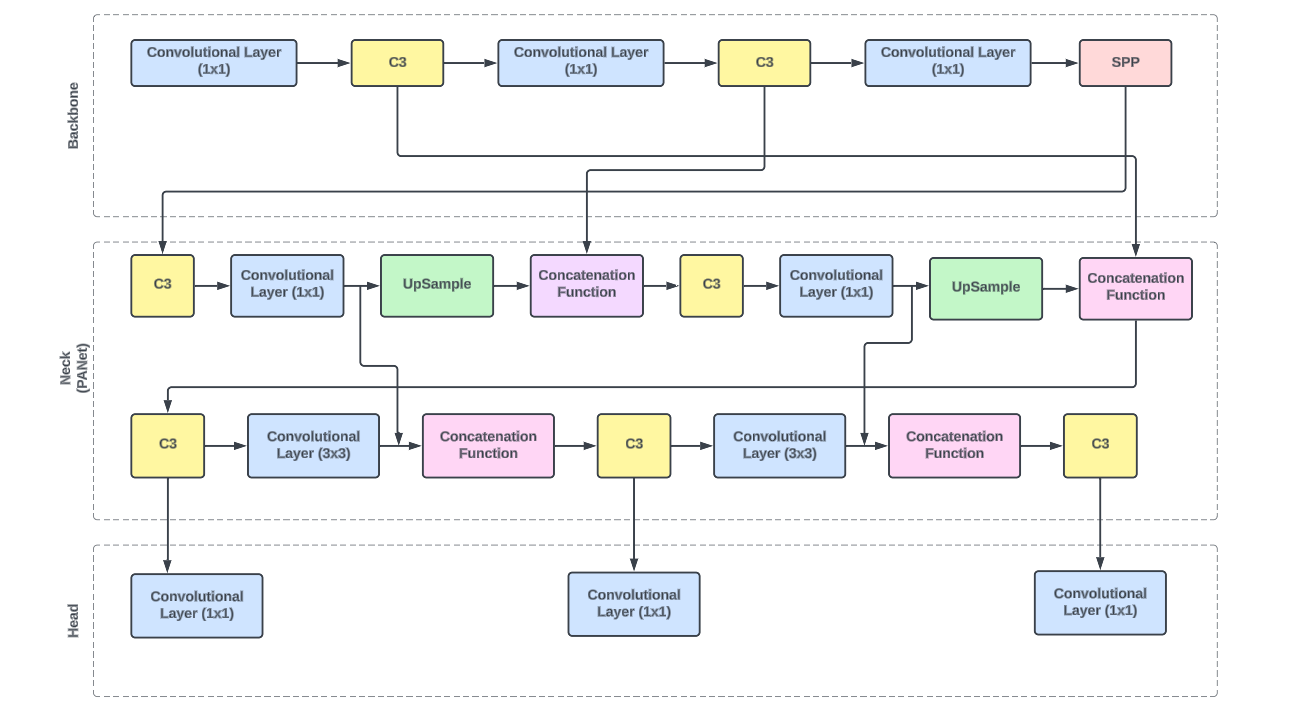
\includegraphics[scale=0.5]{images/methodology/YOLOv5_architecture.png}
\caption{YOLOv5 architecture}
\end{center}
\end{figure}
\par The Yolov5 architecture consists of three parts:
 
\begin{enumerate}
   \item {\bf{ Backbone:}} The task of extracting features from the input image falls to the backbone network. The backbone of YOLOv5 usually consists of a sequence of convolutional layers that increase the number of channels to record hierarchical information while gradually downsampling the input image's spatial dimensions.
   \begin{enumerate}
       \item {\bf{Convolutional layer}}: This layer is responsible for extracting features from the input image by convolving with the kernels.
       \item {\bf{C3}}: Convolutional 3x3 is a specific type of convolutional layer in which 3x3 filters are applied to the input image.
       \par After a set of Convolution layer and C3 the output goes through SPP.
       \item {\bf{SPP}}: Spatial Pyramid Pooling is done which divides the feature maps into sub-regions of various sizes and the pooling operation is done without the need for resizing the image.
   \end{enumerate}
   \item {\bf{ Neck}}: The YOLOv5 architecture's neck functions as a transitional element between the head and the backbone. It is in charge of performing further processing on the characteristics that the backbone has retrieved to improve its representational ability. To enhance the network's capacity to identify objects of different sizes, YOLOv5's neck usually consists of extra convolutional layers, feature pyramid networks (FPNs), or other architectural components that merge features from several scales.\par In this layer Convolution and C3 are done along with Upsampling and application of concatenation function.
   \begin{enumerate}
       \item {\bf{Concatenation function}}: The resultant feature maps from various sub-regions are concatenated together along the depth dimension after applying SPP. Concatenation retains spatial information across many scales by combining the data from these sub-regions into a single feature vector.
       \item {\bf{Upsample}}: Feature maps can have their spatial resolution increased through the technique of upsampling. It means increasing the size of feature maps through the use of interpolation methods like bilinear or nearest-neighbor interpolation, or by adding empty rows and columns (zero-padding). Spatial features lost during downsampling processes, such as max pooling or convolution with stride, can be recovered with the aid of upsampling.
   \end{enumerate}
    \item {\bf{Head}}: The YOLOv5 architecture's head is in charge of producing object detection predictions using the features of the neck and backbone supply. The final output layer, which predicts boundaries, objectness scores, and probabilities of classes for the objects in the input image, usually comes after a series of convolutional layers. Depending on which version of YOLOv5 is being used, the head of the algorithm may incorporate methods like anchor box clustering, sigmoid activation, or softmax for classifying object classes, and prediction of objectness scores.
\end{enumerate}

\newpage
\section {Design and Formulation}
\begin{figure}[H]
\begin{center}
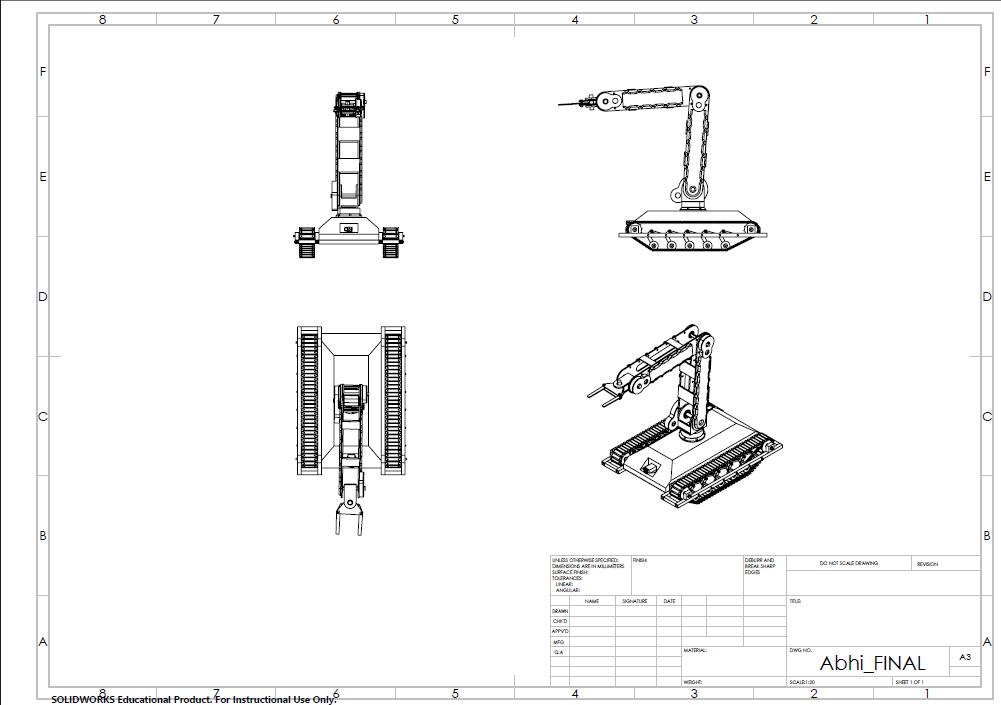
\includegraphics[scale=0.5]{images/design/schematic_diag.png}
\caption{Schematic Diagram}
\end{center}
\end{figure}

\par Above figure illustrates the design for the robot arm and the rover. The self-navigating cotton-picking rover is made up of a wheeled platform for moving through cotton fields. The rover has a hand extension installed that can reach mature cotton bolls on plants and delicately harvest them. The rover's sensors and cameras enable it to capture in-depth images of the cotton plants. These photos are processed in real-time using computer vision algorithms, which allow mature cotton bolls to be distinguished from other plant components including leaves and stems. The computer vision system uses a variety of visual signals, including size, texture, and color, to accurately identify mature cotton bolls. 
Once a mature cotton boll is discovered, the rover's control system decides the optimal route and position for the hand attachment to reach and pick it. The hand extension's actuators allow for the exact and cautious removal. It is set up with defined pathways and obstacle elimination algorithms for efficient field coverage while avoiding collisions with impediments. 

\begin{figure}[H]
\begin{center}
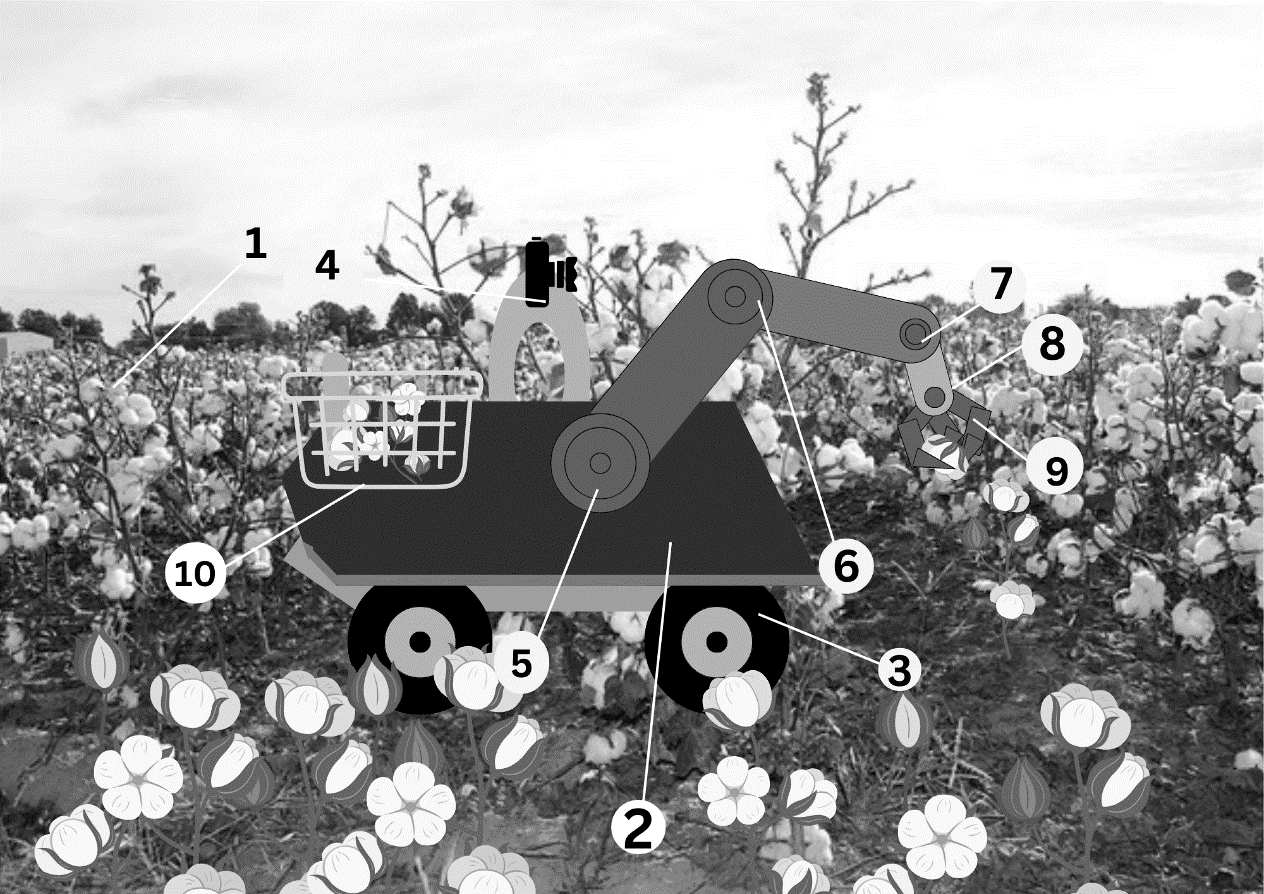
\includegraphics[scale=0.7]{images/design/working.png}
\caption{Working of prototype}
\end{center}
\end{figure}

\par Above figure shows rows of fully grown cotton plants extending into the distance on a cotton field. 
An automatic cotton picking rover is situated among the cotton plants in the image's foreground. The rover is a small, three-wheeled vehicle with a robust structure made for challenging outdoor conditions. 

\section {Objectives completed till date}

\begin{enumerate}
\item  To select an image processing model for the cotton detection in actual condition, which is easy to deploy on any processing device with less specification.

\item  To train the YOLO v5 model to identify and detect cotton boll from the plant when provided with a real-life video feed through a camera module.

\item To design a robot arm to pluck cotton from a plant and store it in a container.

\item To create a robotic arm that, when manually operated, can accomplish particular, coordinated tasks in three dimensions.


\end{enumerate}


\newpage
\section {Flow Chart and algorithm} 
\par The flow chart is as follows:


\par Take pictures of the cotton field with cameras or other video recording equipment.
Make sure there is enough quality in the video to process the images accurately.

{\bf{Picture Division:}}

Divide the photos into segments so that the cotton plants are separated from the surrounding area and other objects.
Convolutional neural networks (CNNs) trained on annotated datasets are a common technique for learning the characteristics of cotton plants.


\begin{figure}[!htb]
\begin{center}
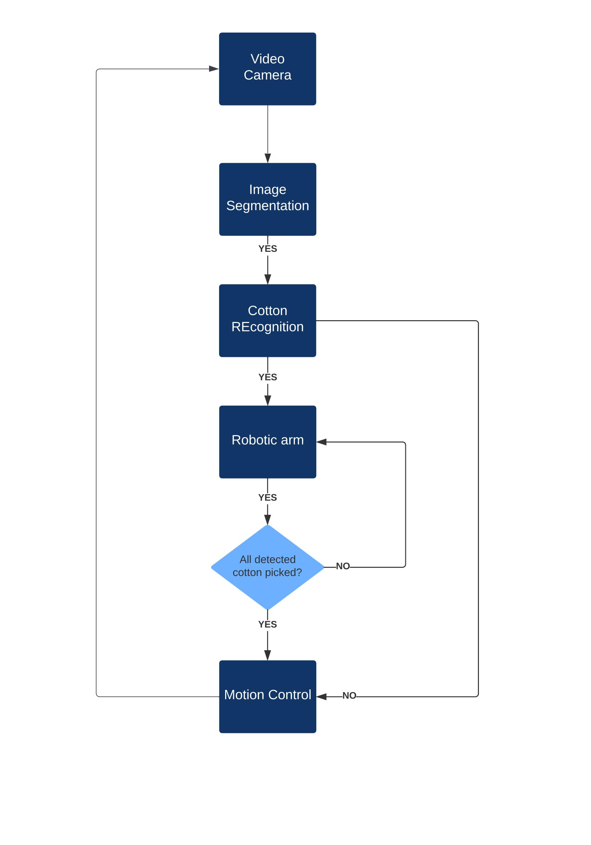
\includegraphics[scale=0.8]{images/diagrams/flowchart.png}
\caption{Flow Chart}
\end{center}
\end{figure}

\newpage

\par {\bf{Recognition of Cotton:}}

For cotton recognition, use a deep learning model.
Train the model to discriminate between various cotton plant components, particularly the cotton bolls.
Individual cotton bolls within the segmented images can be recognized and located using characteristics like color, texture, and shape.
\par {\bf{Arm Control via Robots:}}

Apply control algorithms to convert the locations of cotton bolls that have been identified into accurate robotic arm movements.
To account for changes in the positions of the plant and cotton, take into consideration feedback mechanisms like sensors on the robotic arm.

\par {\bf{Picking Cotton:}}

Create a mechanism for the robotic arm's end effector—the portion that interacts with the surroundings—to delicately pick up and remove the cotton bolls.
Use a grasping device that can adjust to the various sizes and positions of cotton bolls.

 {\bf{Iterative Method:}}

Repeat the entire procedure for every frame in the movie or every plant in the field.
Use real-time processing to adjust to conditions that change, such as shifts in plant growth and lighting.





\chapter{Results and Discussions}




\section {Hardware Setup}

\par The Cotton Picking Robot has extensive hardware in the Robotic body where three different types of motors are used, these motors are controlled using a motor driver whose current rating is more than 5 Amperes.

\subsection {Hardware Components and Specifications}
\begin{itemize}
\item {\bf{Arduino Mega}}

\begin{figure}[H]
\begin{center}
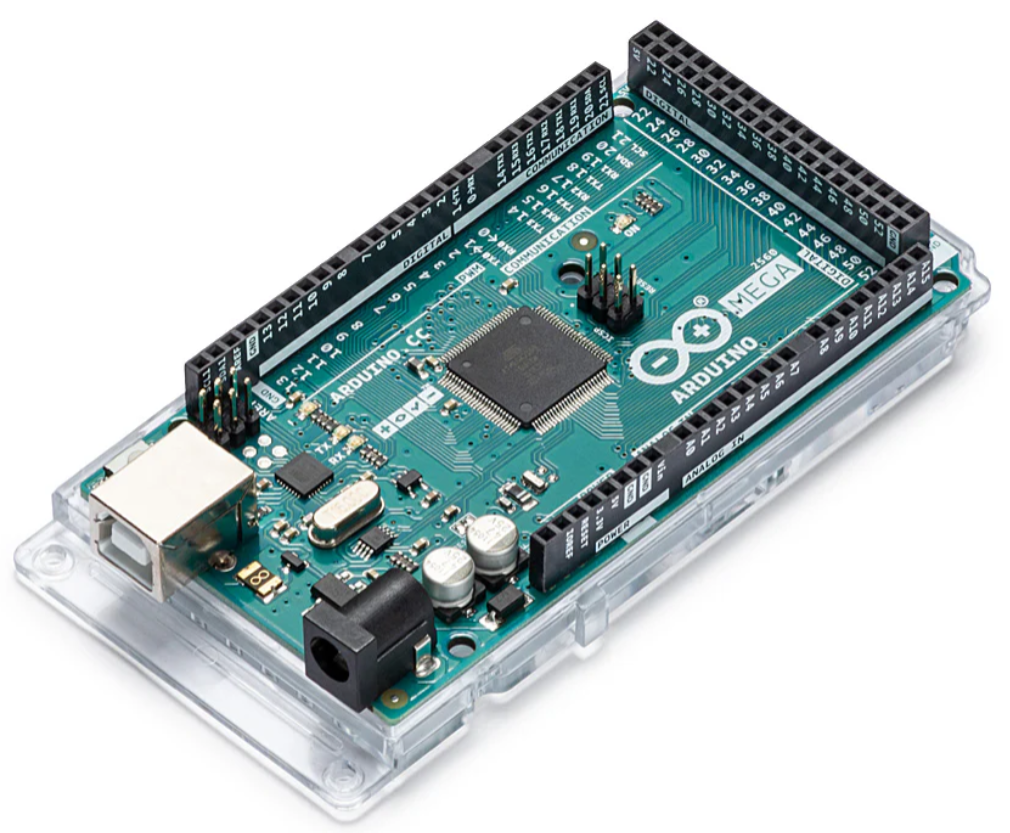
\includegraphics[scale=0.35]{images/hardware/Arduinomega.png}
\caption{Arduino Mega}
\end{center}
\end{figure}

\par The Arduino Mega is a microcontroller board that is built around the ATmega2560. This board is perfect for more complicated projects because it has a lot more power than many other Arduino boards. With its huge memory capacity, it can accommodate more variables and larger programs. Temperature, potentiometer, and light sensors are just a few examples of the sensors that may be connected to the Arduino Mega's 16 analog inputs. It also has 54 digital pins for input and output (I/O), 15 of which can be utilized as outputs for pulse width modulation, or PWM. It can manage numerous components at once, including LEDs, relays, buttons, and screens, because to its huge number of I/O pins. 



\begin{table}[H]
\begin{center}
\caption{Specifications of Arduino Mega}% title of Table
\hspace*{0.2in}
\\
\begin{tabular}{| p{5cm} | p{5cm} |}
\hline
{\bf{Parameter}}             &{\bf{Value}}           \\ \hline
Operating voltage
& 5V \\ \hline

Analog input pins
& 16 \\ \hline

Digital I/O pins
& 54 \\ \hline

Clock speed
& 16 MHz \\ \hline

Flash memory
& 256 KB \\ \hline
\end{tabular}
\end{center}
\end{table}


\newpage
\item {\bf{Servo Driver}}
\begin{figure}[!htb]
\begin{center}
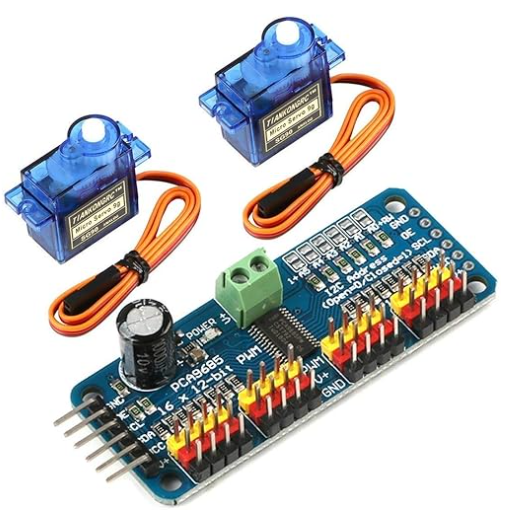
\includegraphics[scale=0.5]{images/hardware/16channel PWM.png}
\caption{16-channel 12-bit PWM servo driver}
\end{center}
\end{figure}

\par A compact module, the 16-channel 12-bit PWM servo driver, has the ability to precisely control several servo motors. Using pulse-width modulation (PWM) signals, it precisely places servos, offering 12-bit resolution for more fluid motions. For robotics and automation applications, precise motion control—which can manage up to 16 servos independently—is essential.

\begin{table}[H]
\begin{center}
\newpage
\caption{Specifications of Servo Driver}% title of Table
\hspace*{0.2in}
\\
\begin{tabular}{| p{5cm} | p{5cm} |}
\hline
{\bf{Parameter}}             &{\bf{Value}}           \\ \hline
Chip
& PCA9685 \\ \hline

Number of channels
& 16 \\ \hline

Resolution
& 12-bit \\ \hline

PWM frequency range
& 40 Hz to 1000 Hz \\ \hline

\end{tabular}
\end{center}
\end{table}




\newpage
\item {\bf{Servo Motor}}
\begin{figure}[!htb]
\begin{center}
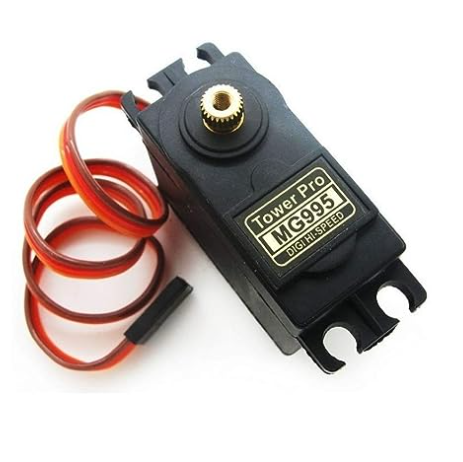
\includegraphics[scale=0.6]{images/hardware/Servo995.png}
\caption{Servo 995}
\end{center}
\end{figure}

\par The Servo 995 is a standard-sized servo motor that is well-known for its dependability and adaptability. It operates at 4.8V to 6V and has a torque range suitable for many robotic and hobbyist applications. Its widely compatible standard servo interface is used by both animatronics and model airplanes.

\begin{table}[H]
\begin{center}
\caption{Specifications of Servo 995}% title of Table
\hspace*{0.2in}
\\
\begin{tabular}{| p{5cm} | p{5.5cm} |}
\hline
{\bf{Parameter}}             &{\bf{Value}}           \\ \hline
Operating voltage
& 4.8V - 7.2V \\ \hline

Rotation range
& 180° \\ \hline

Motor type
& DC Motor \\ \hline

Connector type
& 3-pin (Power, Ground, Signal) \\ \hline

\end{tabular}
\end{center}
\end{table}



% \item {\bf{}}
\begin{figure}[H]
\begin{center}
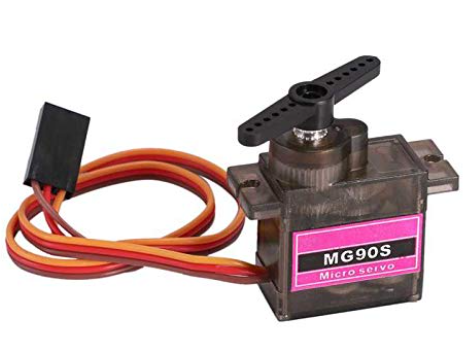
\includegraphics[scale=0.7]{images/hardware/servo mg90s.png}
\caption{Servo MG90s}
\end{center}
\end{figure}

\par The MG90s and other small servo motors are renowned for their small size and light weight. Because it can run on 4.8 to 6 volts and has respectable torque and speed performance, it is appropriate for small-scale robotics and radio control projects.

\begin{table}[H]
\begin{center}
\caption{Specifications of Servo MG90s}% title of Table
\hspace*{0.2in}
\\
\begin{tabular}{| p{5cm} | p{5cm} |}
\hline
{\bf{Parameter}}             &{\bf{Value}}           \\ \hline
Operating voltage
& 4.8V - 6V \\ \hline

Dead bandwidth
& 5 µs \\ \hline

Rotation range
& 180° \\ \hline

Operating temp. range
& -30°C to +60°C \\ \hline

\end{tabular}
\end{center}
\end{table}


% \item {\bf{}}
\begin{figure}[H]
\begin{center}
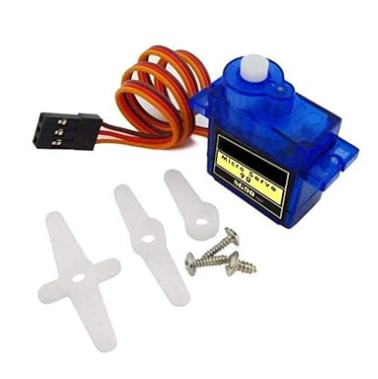
\includegraphics[scale=0.7]{images/hardware/Servo sg90.png}
\caption{Servo SG90}
\end{center}
\end{figure}

\par The SG90 micro servo's lightweight and compact design makes it an affordable choice. Operating at 4.8V to 6V, its modest torque and speed make it perfect for little mechanical jobs, remote control vehicles, and lightweight robotics applications.

\begin{table}[H]
\begin{center}
\caption{Specifications of Servo SG90}% title of Table
\hspace*{0.2in}
\\
\begin{tabular}{| p{5cm} | p{5cm} |}
\hline
{\bf{Parameter}}             &{\bf{Value}}           \\ \hline
Operating voltage
& 4.8V - 6V \\ \hline

Weight
& 9 grams \\ \hline

Dead bandwidth
& 10 µs \\ \hline

Gear Type
& Plastic \\ \hline

\end{tabular}
\end{center}
\end{table}

\newpage
\item {\bf{Power Supply}}
\begin{figure}[!htb]
\begin{center}
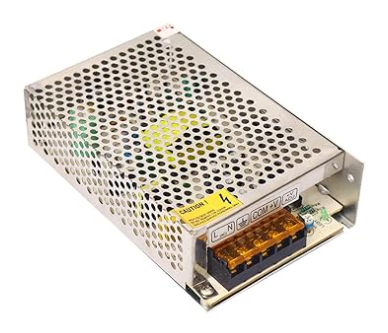
\includegraphics[scale=0.8]{images/hardware/smps 12v,5a.png}
\caption{SMPS 12v,5A }
\end{center}
\end{figure}

SMPS 12V, 5A, often known as switched mode power supply, is a compact and efficient power source. Its maximum current capacity of 5 amps and its consistent 12 volt output make it suitable for a wide range of DIY projects and electronics. Its switching technique ensures minimal heat generation and optimal energy efficiency.


\item {\bf{Connecting Wires}}
\begin{figure}[H]
\begin{center}
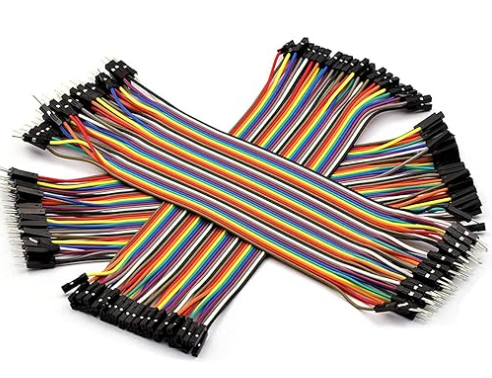
\includegraphics[scale=0.5]{images/hardware/jumper cable.png}
\caption{Jumper cable}
\end{center}
\end{figure}


\end{itemize}

\newpage

\section {Software Setup}


\begin{itemize}
    \item {\bf{Initial Setup}}
    \begin{figure}[!htb]
\begin{center}
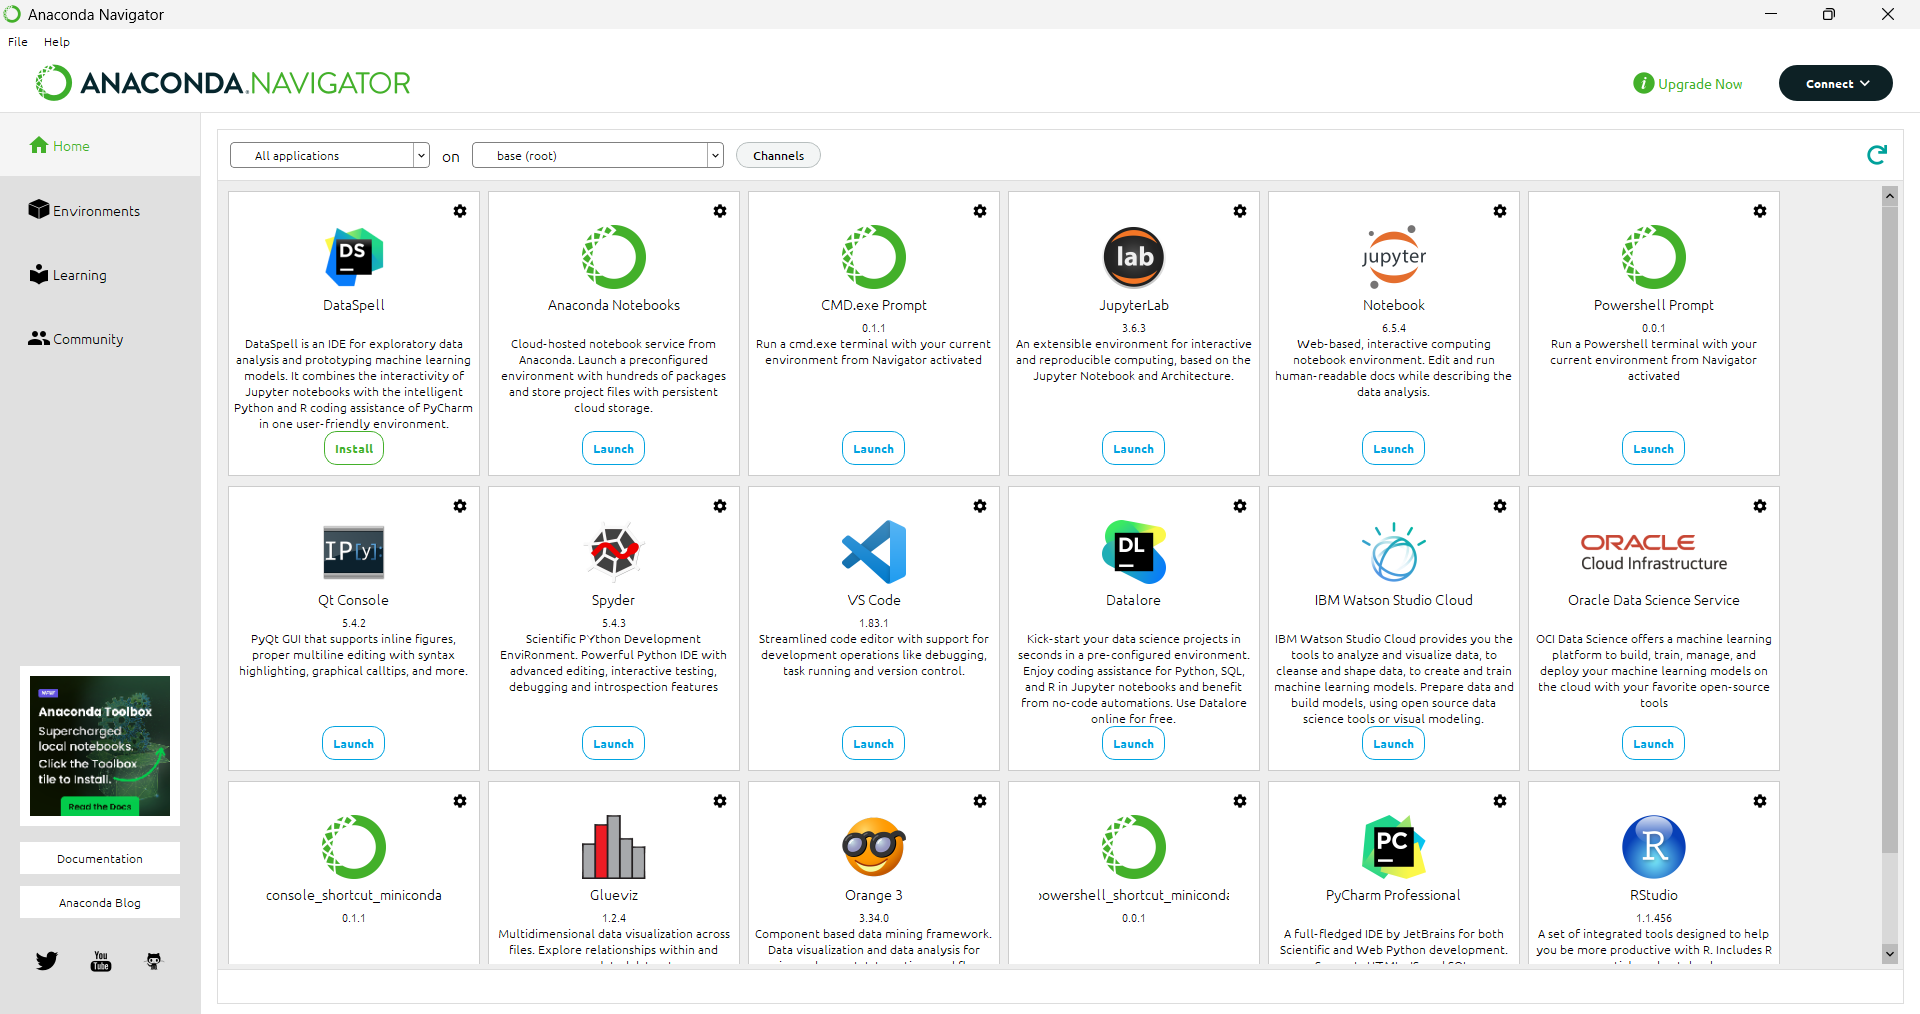
\includegraphics[scale=0.3]{images/platform_SS/Screenshot (6).png}
\caption{Anaconda Dashboard}
\end{center}
\end{figure}

\par Install Anaconda on your laptop first, then set up an environment within it. Running on Linux, macOS, and Windows, Conda is an open-source package and environment management system. Conda installs, runs, and updates dependencies and packages quickly. On your own computer, it also makes it simple to build, save, load, and move between environments. Although it may package and deliver software for any language, it was designed for Python projects.



% \newpage
\item {\bf{Jupyter Notebook }}

\begin{figure}[!htb]
\begin{center}
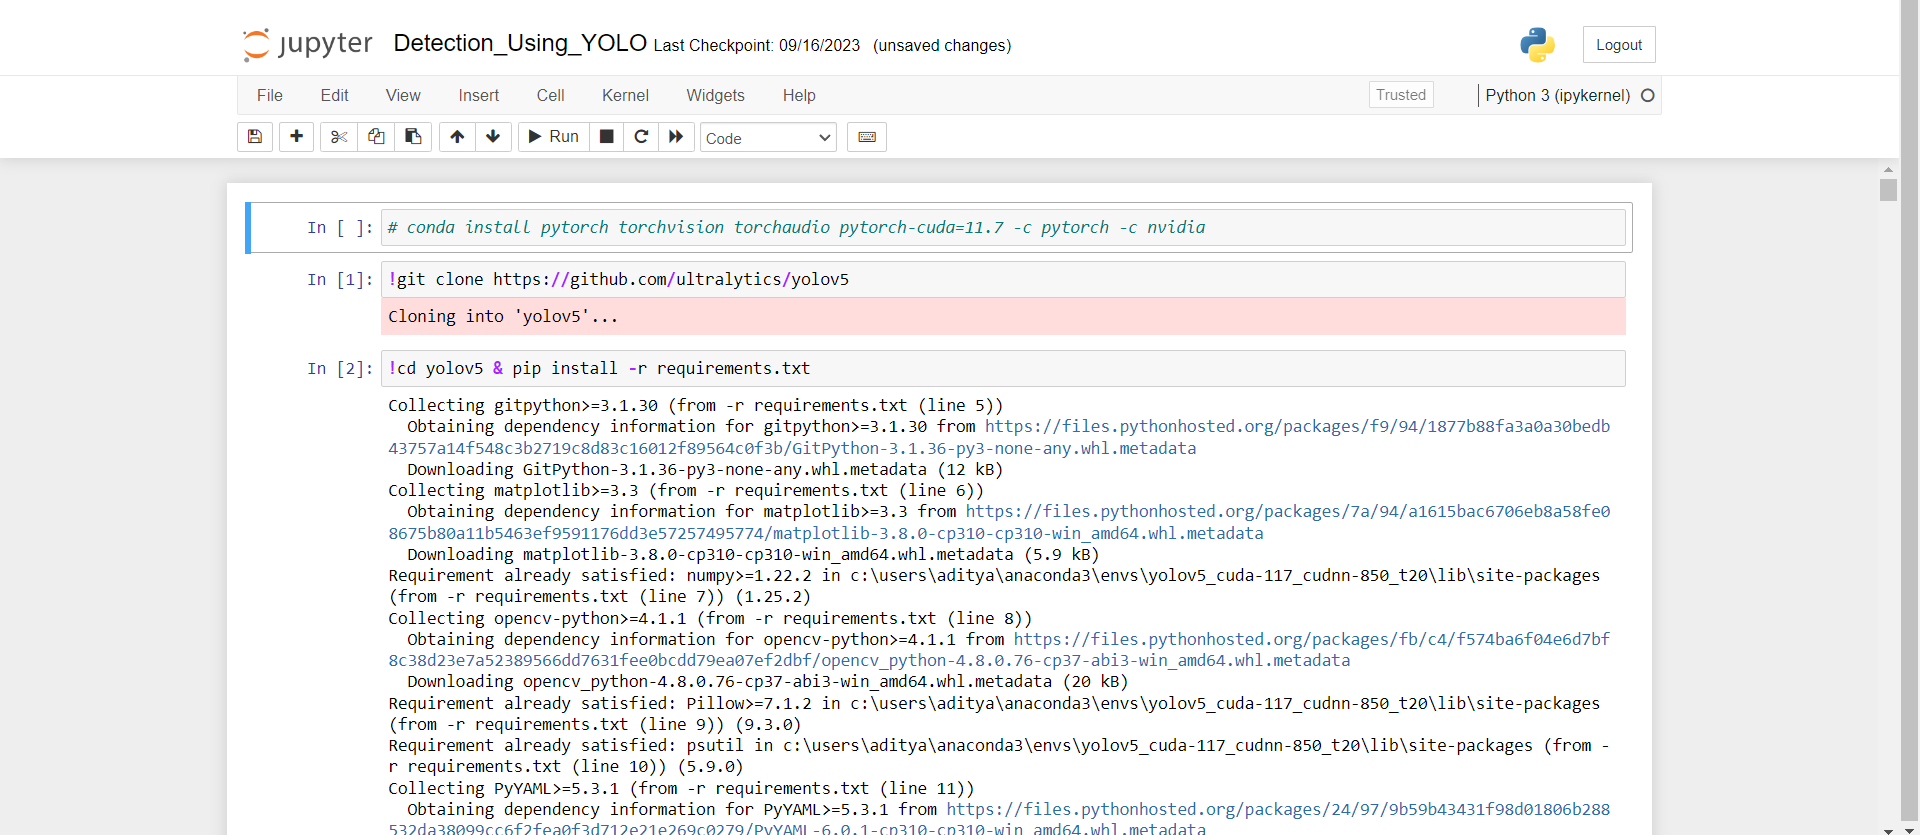
\includegraphics[scale=0.3]{images/platform_SS/Screenshot (3).png}
\caption{Jupyter Dashboard}
\end{center}
\end{figure}


\par You may create and share documents with live code, equations, graphics, and narrative text using the well-known open-source web program Jupyter Notebook. For interactive computing and prototyping, it is extensively utilized in data science and machine learning. There are many different frameworks and packages available for Jupyter Notebook object identification, but TensorFlow or PyTorch for Python is one of the most popular options.




\par To ensure that all of the processing is done on the GPU, install Jupyter Notebook in the environment that has been built and add the file locations for Yolov5, Cuda, and Cudnn. Data scientists can create and share documents with live code, equations, and other multimedia elements using Jupyter Notebook, an open-source web tool.



\item {\bf{PyTorch }}


\begin{figure}[!htb]
\begin{center}
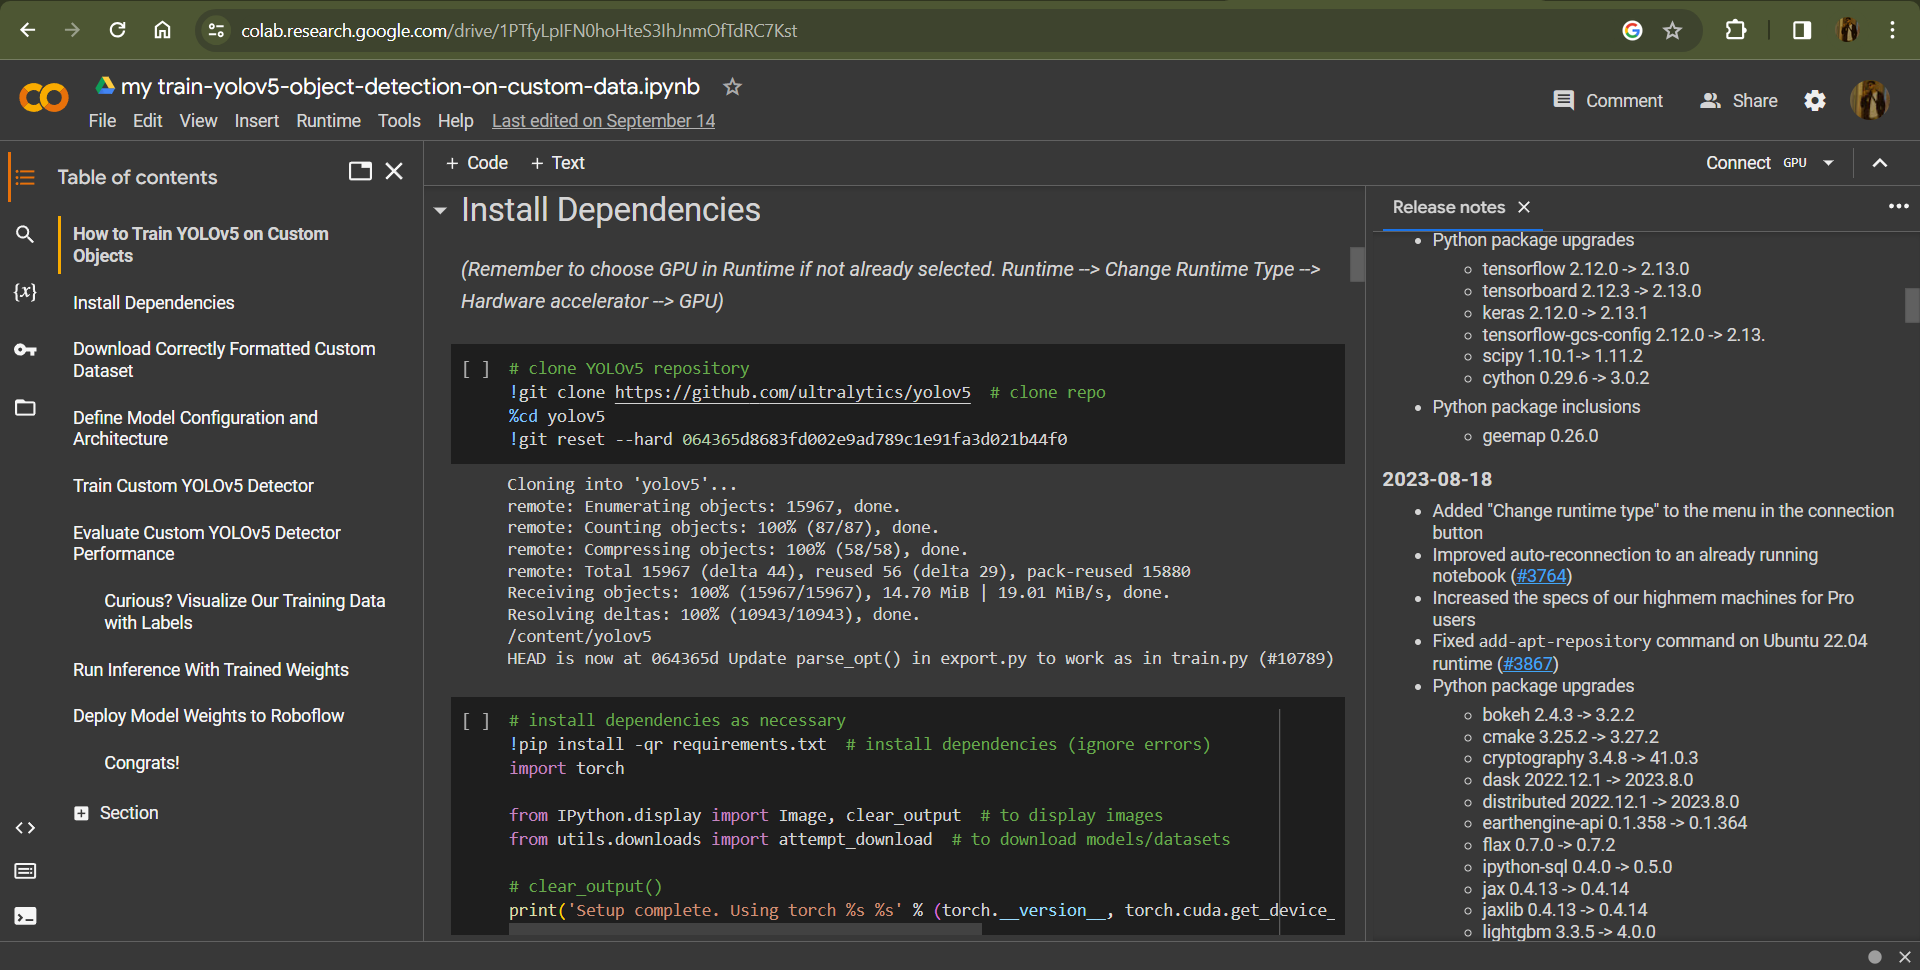
\includegraphics[scale=0.3]{images/platform_SS/Screenshot (5).png}
\caption{Google Colab }
\end{center}
\end{figure}


\par Install the relevant Pytorch version on the machine. PyTorch is a feature-rich framework for creating deep learning models, a kind of machine learning that's frequently applied to tasks like language processing and picture identification. Most machine learning developers find it reasonably easy to understand and use because it is written in Python. 

\item {\bf{Arduino IDE }}

\par Writing, editing, and uploading code to Arduino boards is done with the software program known as the Arduino Integrated Development Environment (IDE). It has a code editor with syntax highlighting for creating sketches, or programs that are developed with functions like setup() and loop(). Users can choose the right board and communication port for their projects by using the IDE's support for numerous built-in and external libraries. Verifying, assembling, and uploading code to the Arduino hardware are important tasks. The IDE also offers a serial monitor to facilitate communication between the board and the computer, as well as a ton of tutorials and example sketches to help with learning. With compatibility for Windows, macOS, and Linux, the Arduino IDE's open-source design makes it a popular and adaptable option.


\begin{figure}[!htb]
\begin{center}
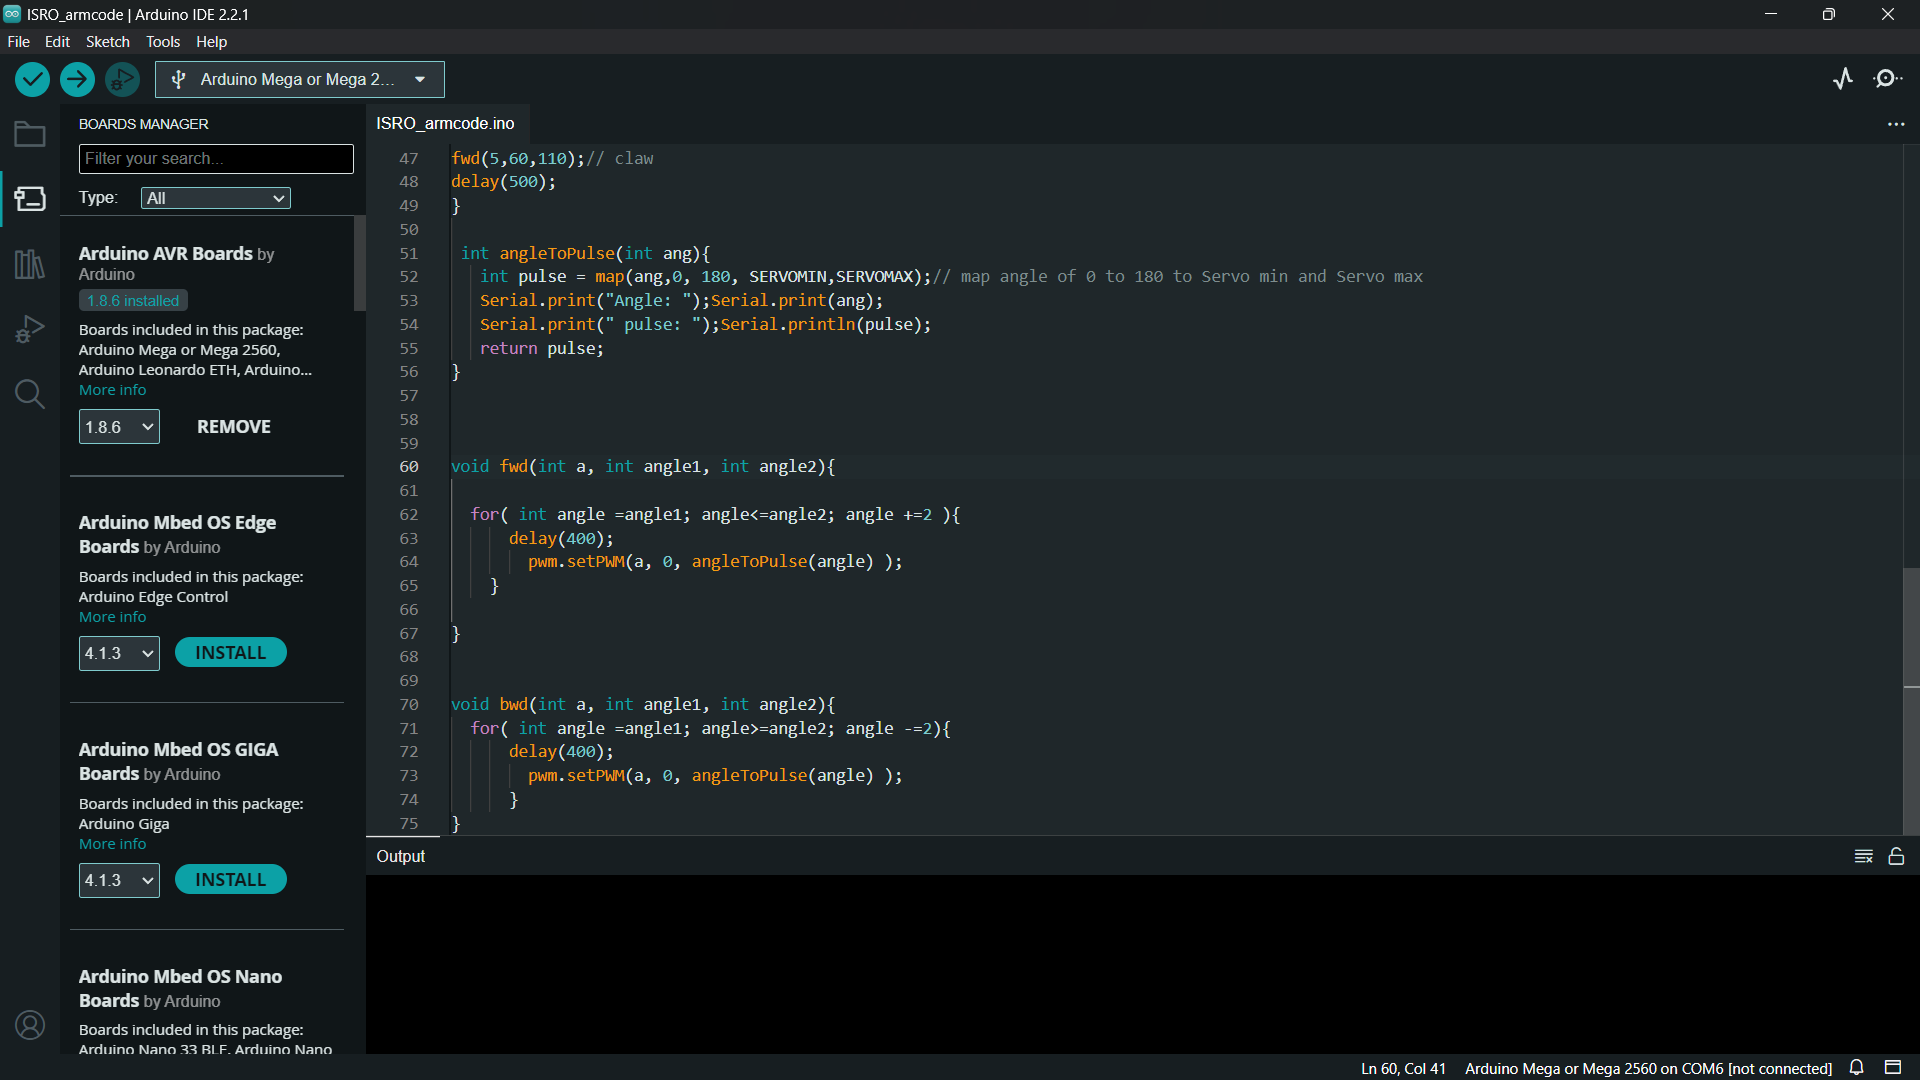
\includegraphics[scale=0.2]{images/platform_SS/Screenshot (45).png}
\caption{Arduino IDE }
\end{center}
\end{figure}








\end{itemize}





\newpage



\section {Results}
\begin{enumerate}
\item {\bf{Software Results}}

\par The confusion matrix of our model is specified in Figure. A confusion matrix, also called an error matrix, is a specific table arrangement used in the field of machine learning, specifically for statistical classification problems. It makes the performance of an algorithm easier to visualize. Typically, this algorithm is supervised learning; in unsupervised learning, it is commonly referred to as a matching matrix

\begin{figure}[!htb]
\begin{center}
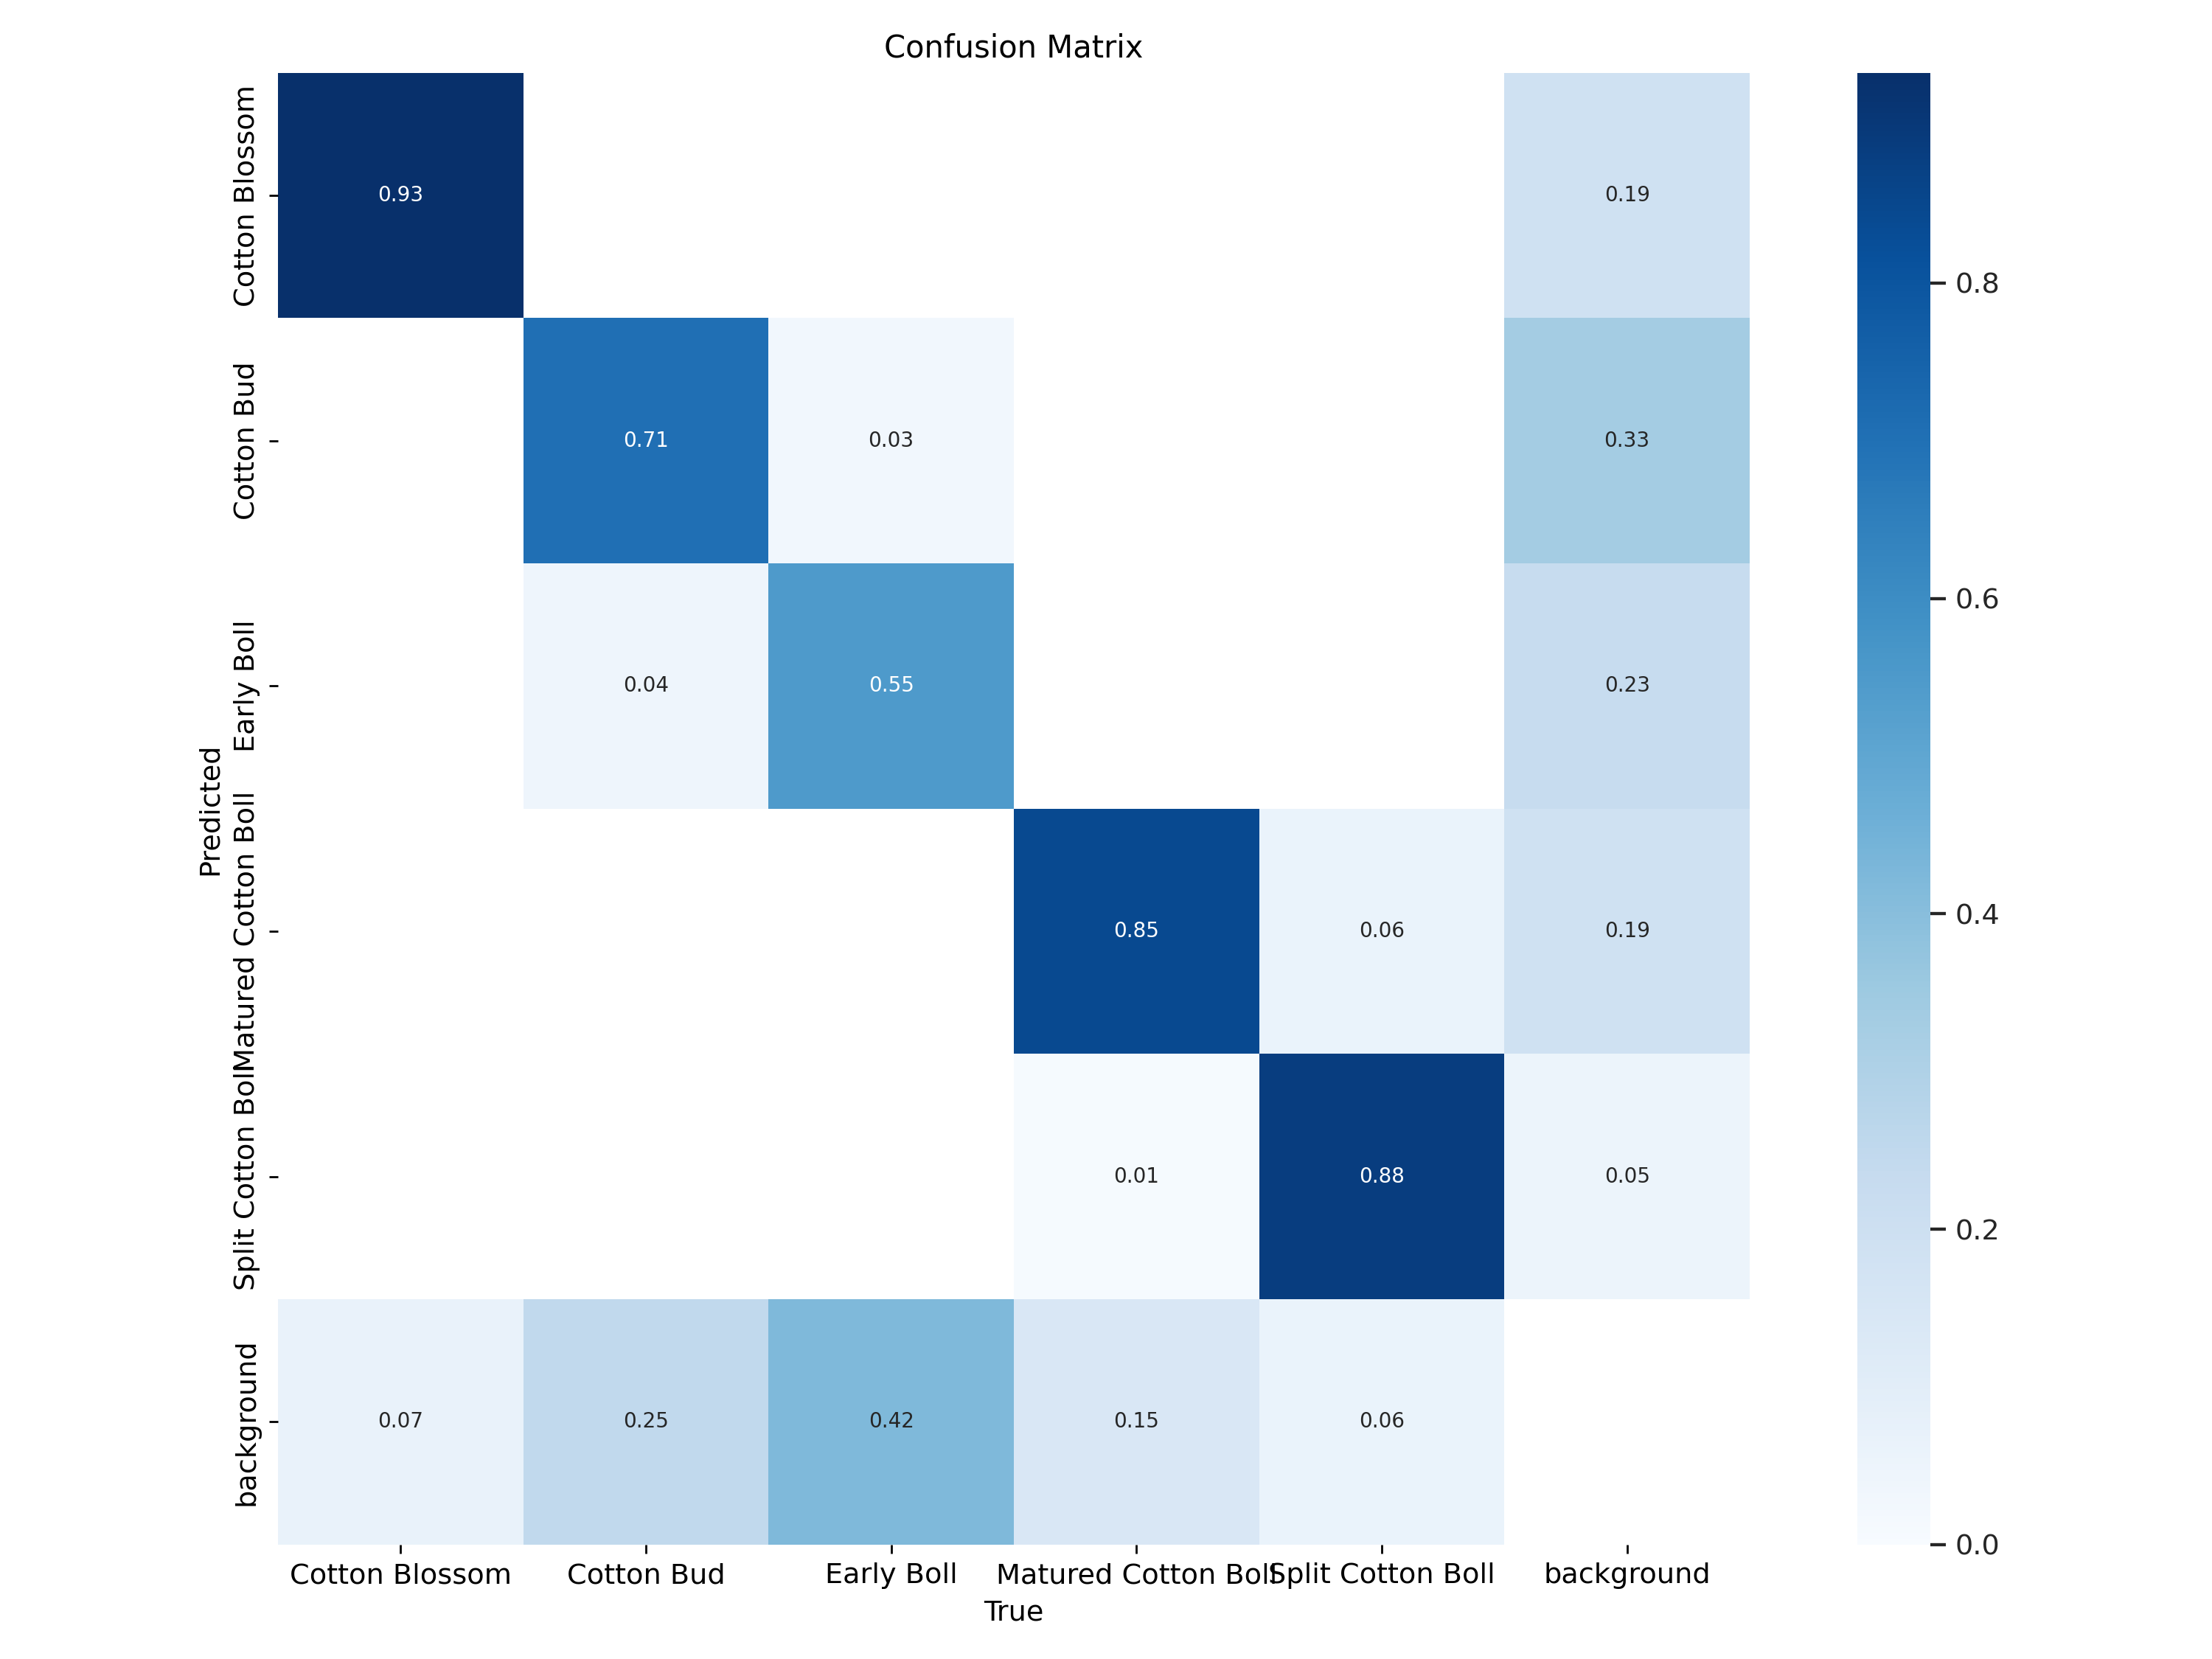
\includegraphics[scale=0.5]{images/results/confusion_matrix.png}
\caption{Confusion Matrix}
\end{center}
\end{figure}

\par From Figure 4.12 we can see from the confusion matrix that the true value for the cotton blossom matches the projected values by 0.93 times, the true value for the bud matches by 0.71 times, and the true value for the early boll matches by 0.55 times. Both the split cotton forecast and the matured boll prediction match the true value by 0.88 times and 0.85, respectively. The background influences the values of the cotton buds and the early boll.

\begin{figure}[!htb]
\begin{center}
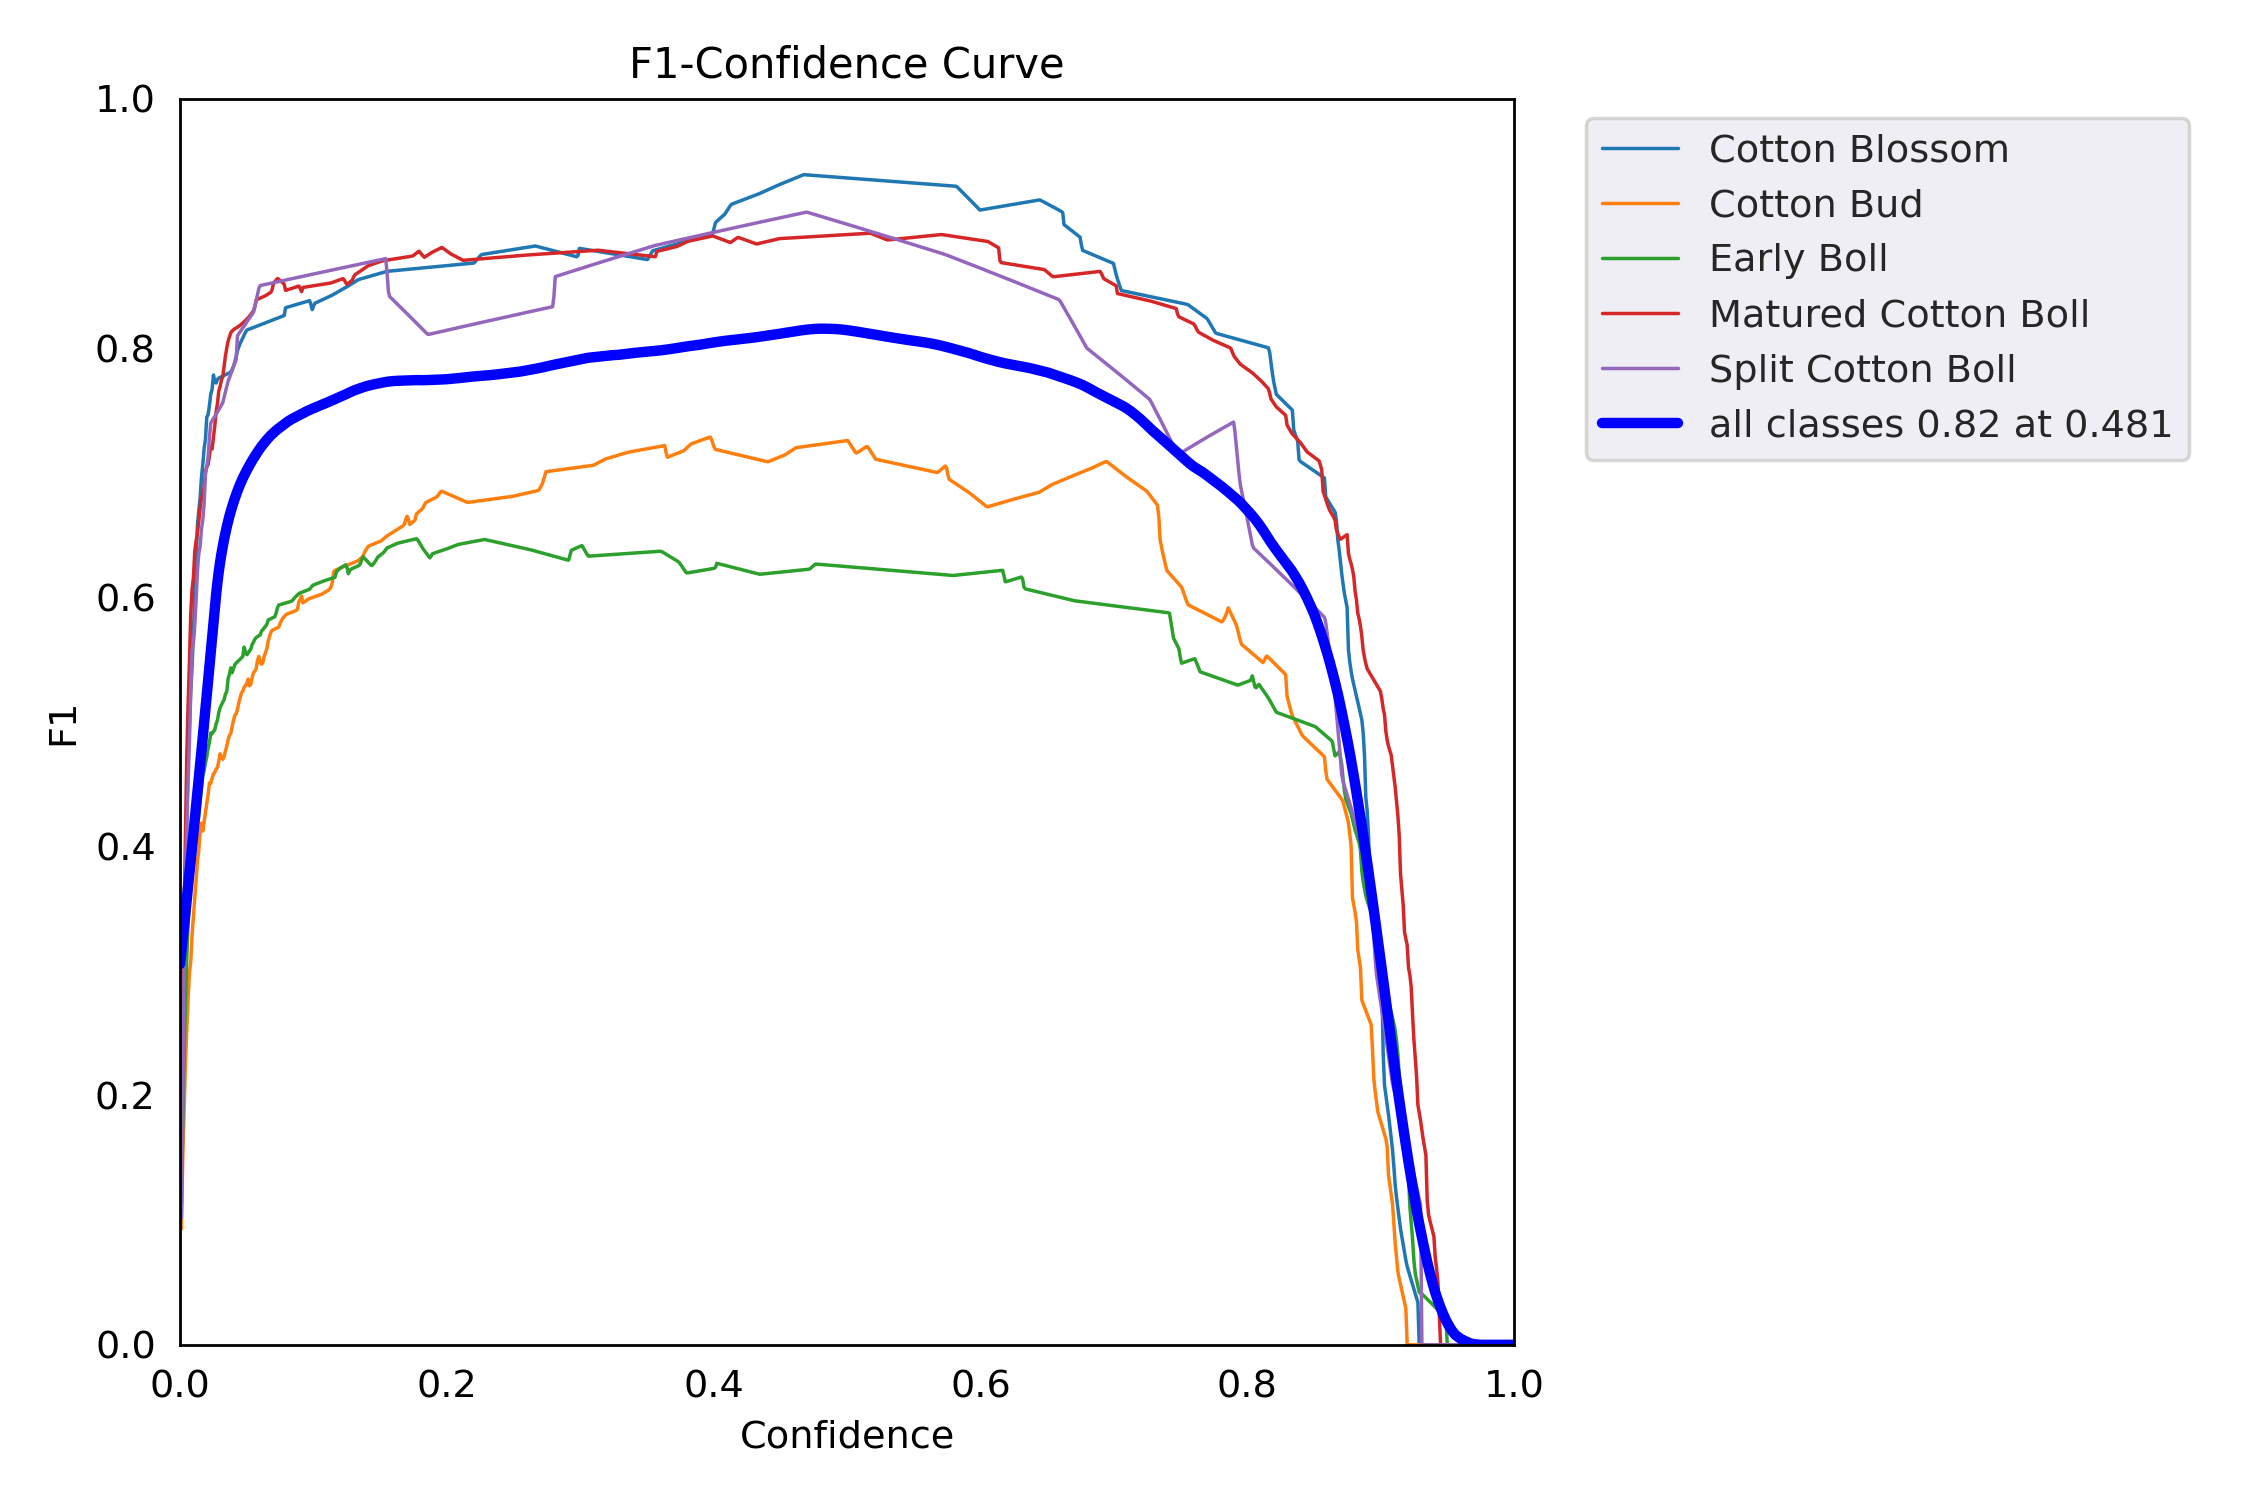
\includegraphics[scale=0.6]{images/results/F1_curve.png}
\caption{F1 confidence curve}
\end{center}
\end{figure}

\par In Figure 4.13, the F1 curve as a reference for all classes, the confidence value of 0.481 maximizes both precision and recall. A greater confidence value is preferred in many situations. This model's confidence value must be 0.8, which isn't far from its highest confidence of 0.82.

\begin{figure}[!htb]
\begin{center}
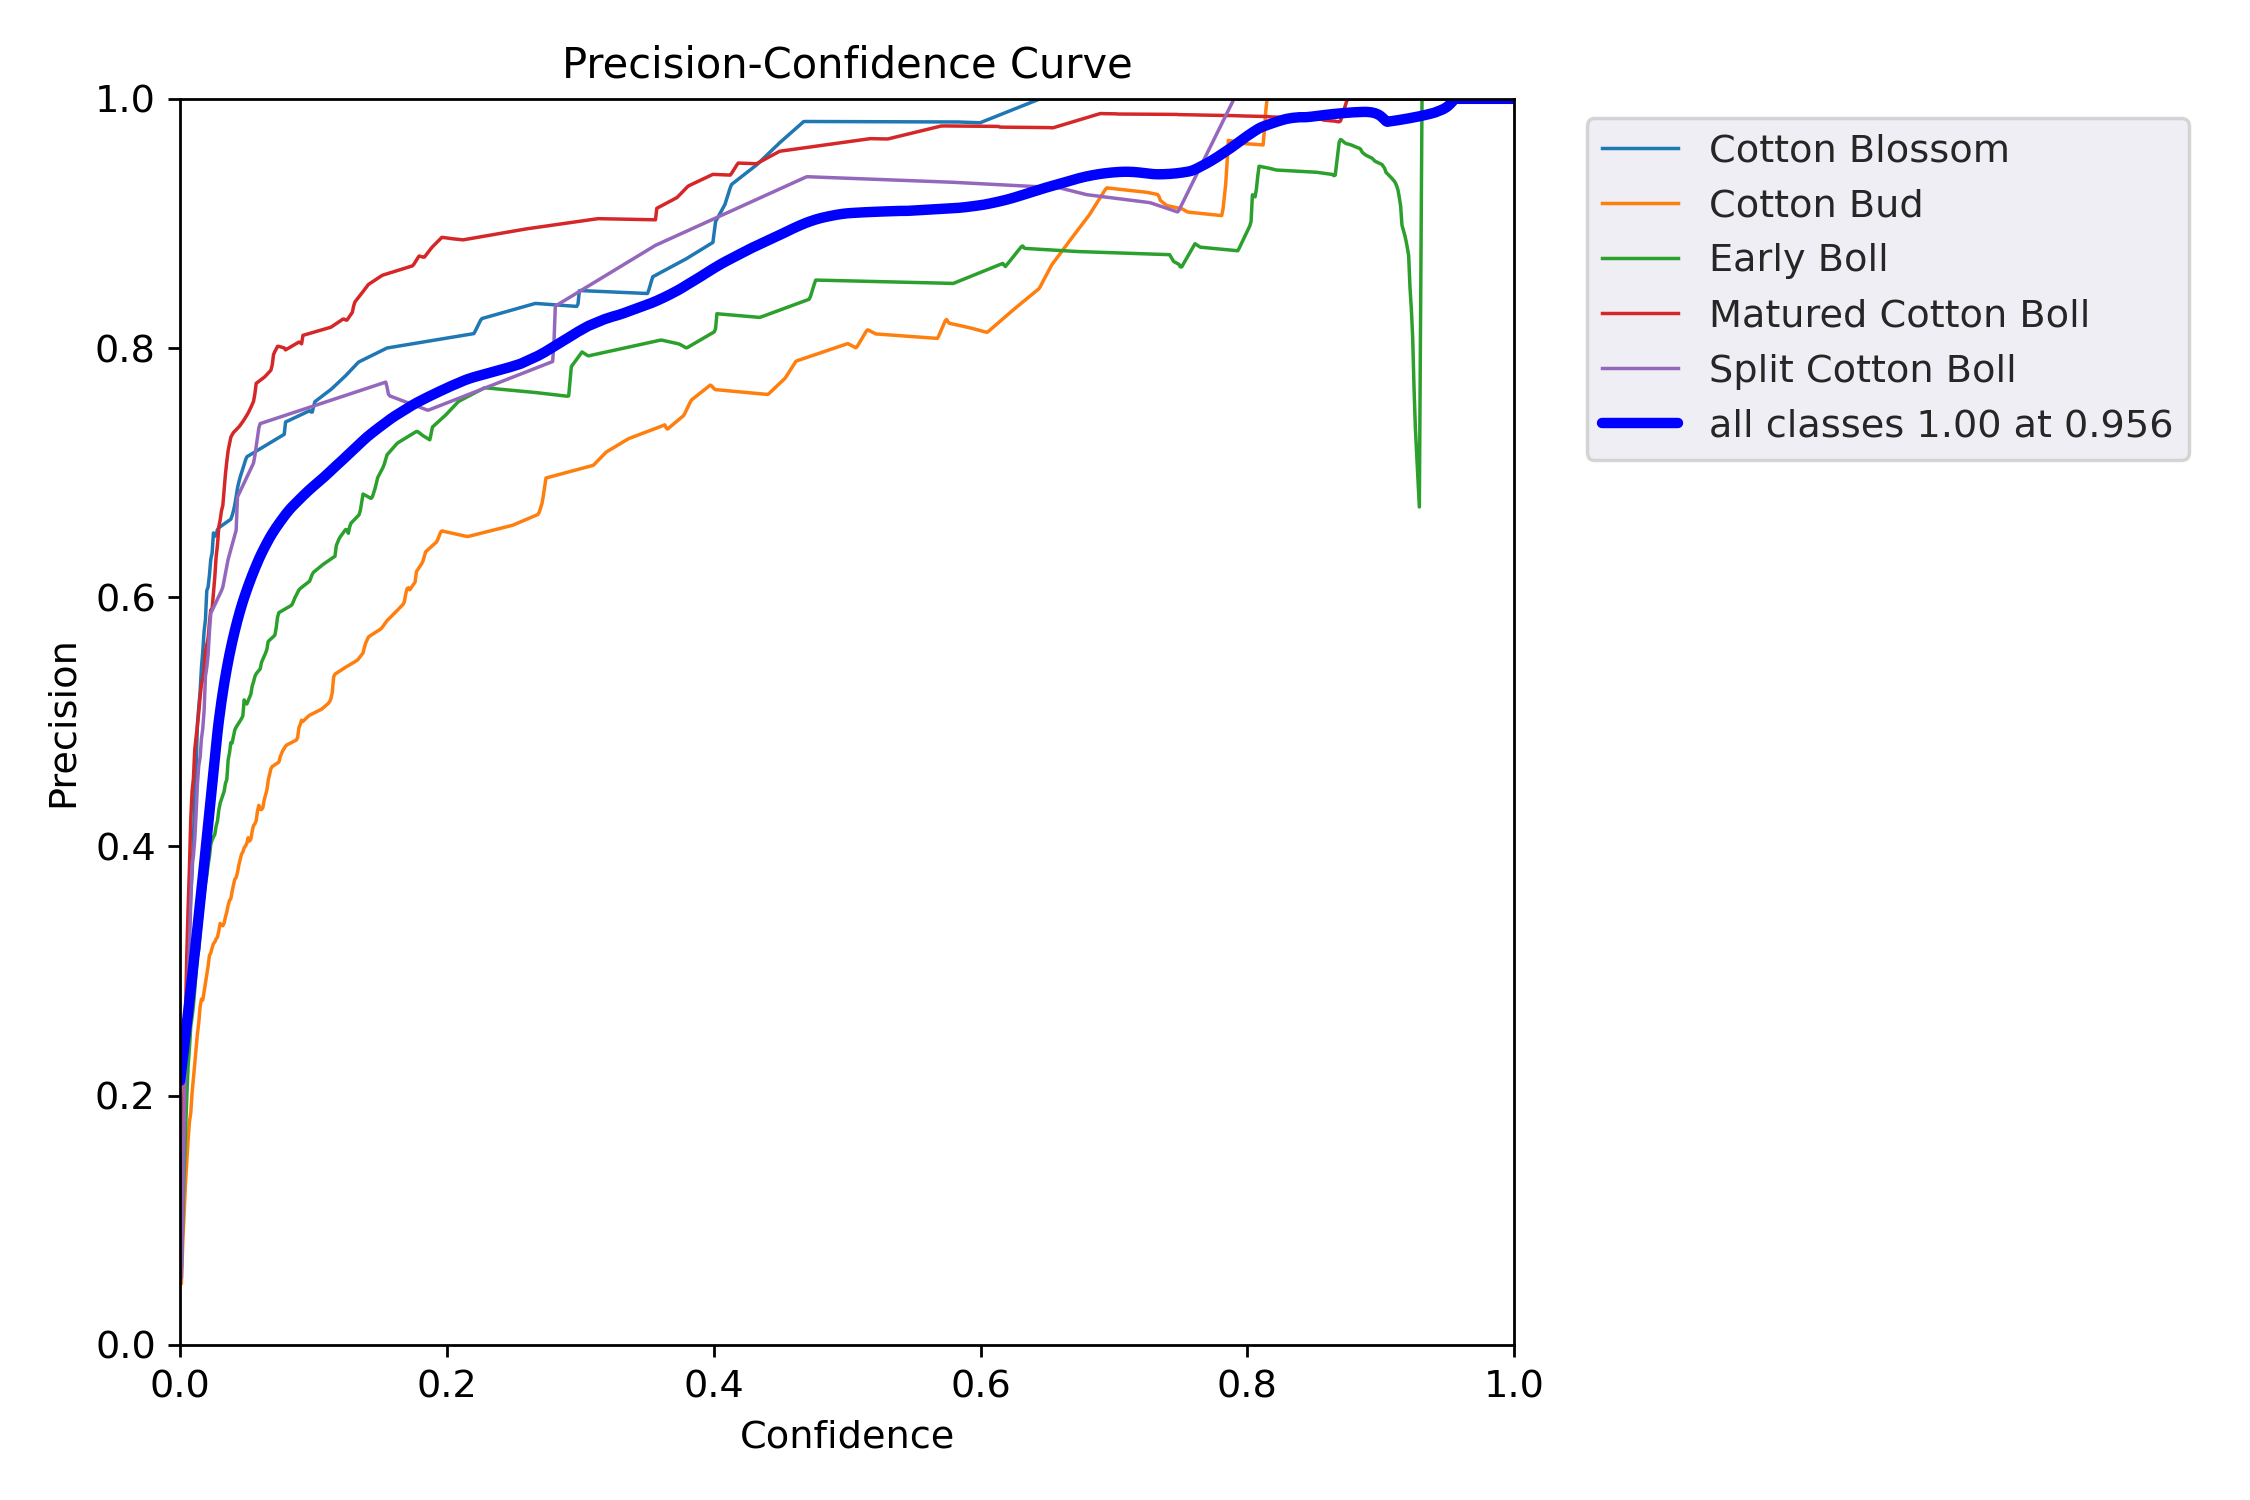
\includegraphics[scale=0.6]{images/results/P_curve.png}
\caption{Precision confidence curve}
\end{center}
\end{figure}

\par Above figure  illustrates the relationship between the model's confidence and precision.

\begin{figure}[!htb]
\begin{center}
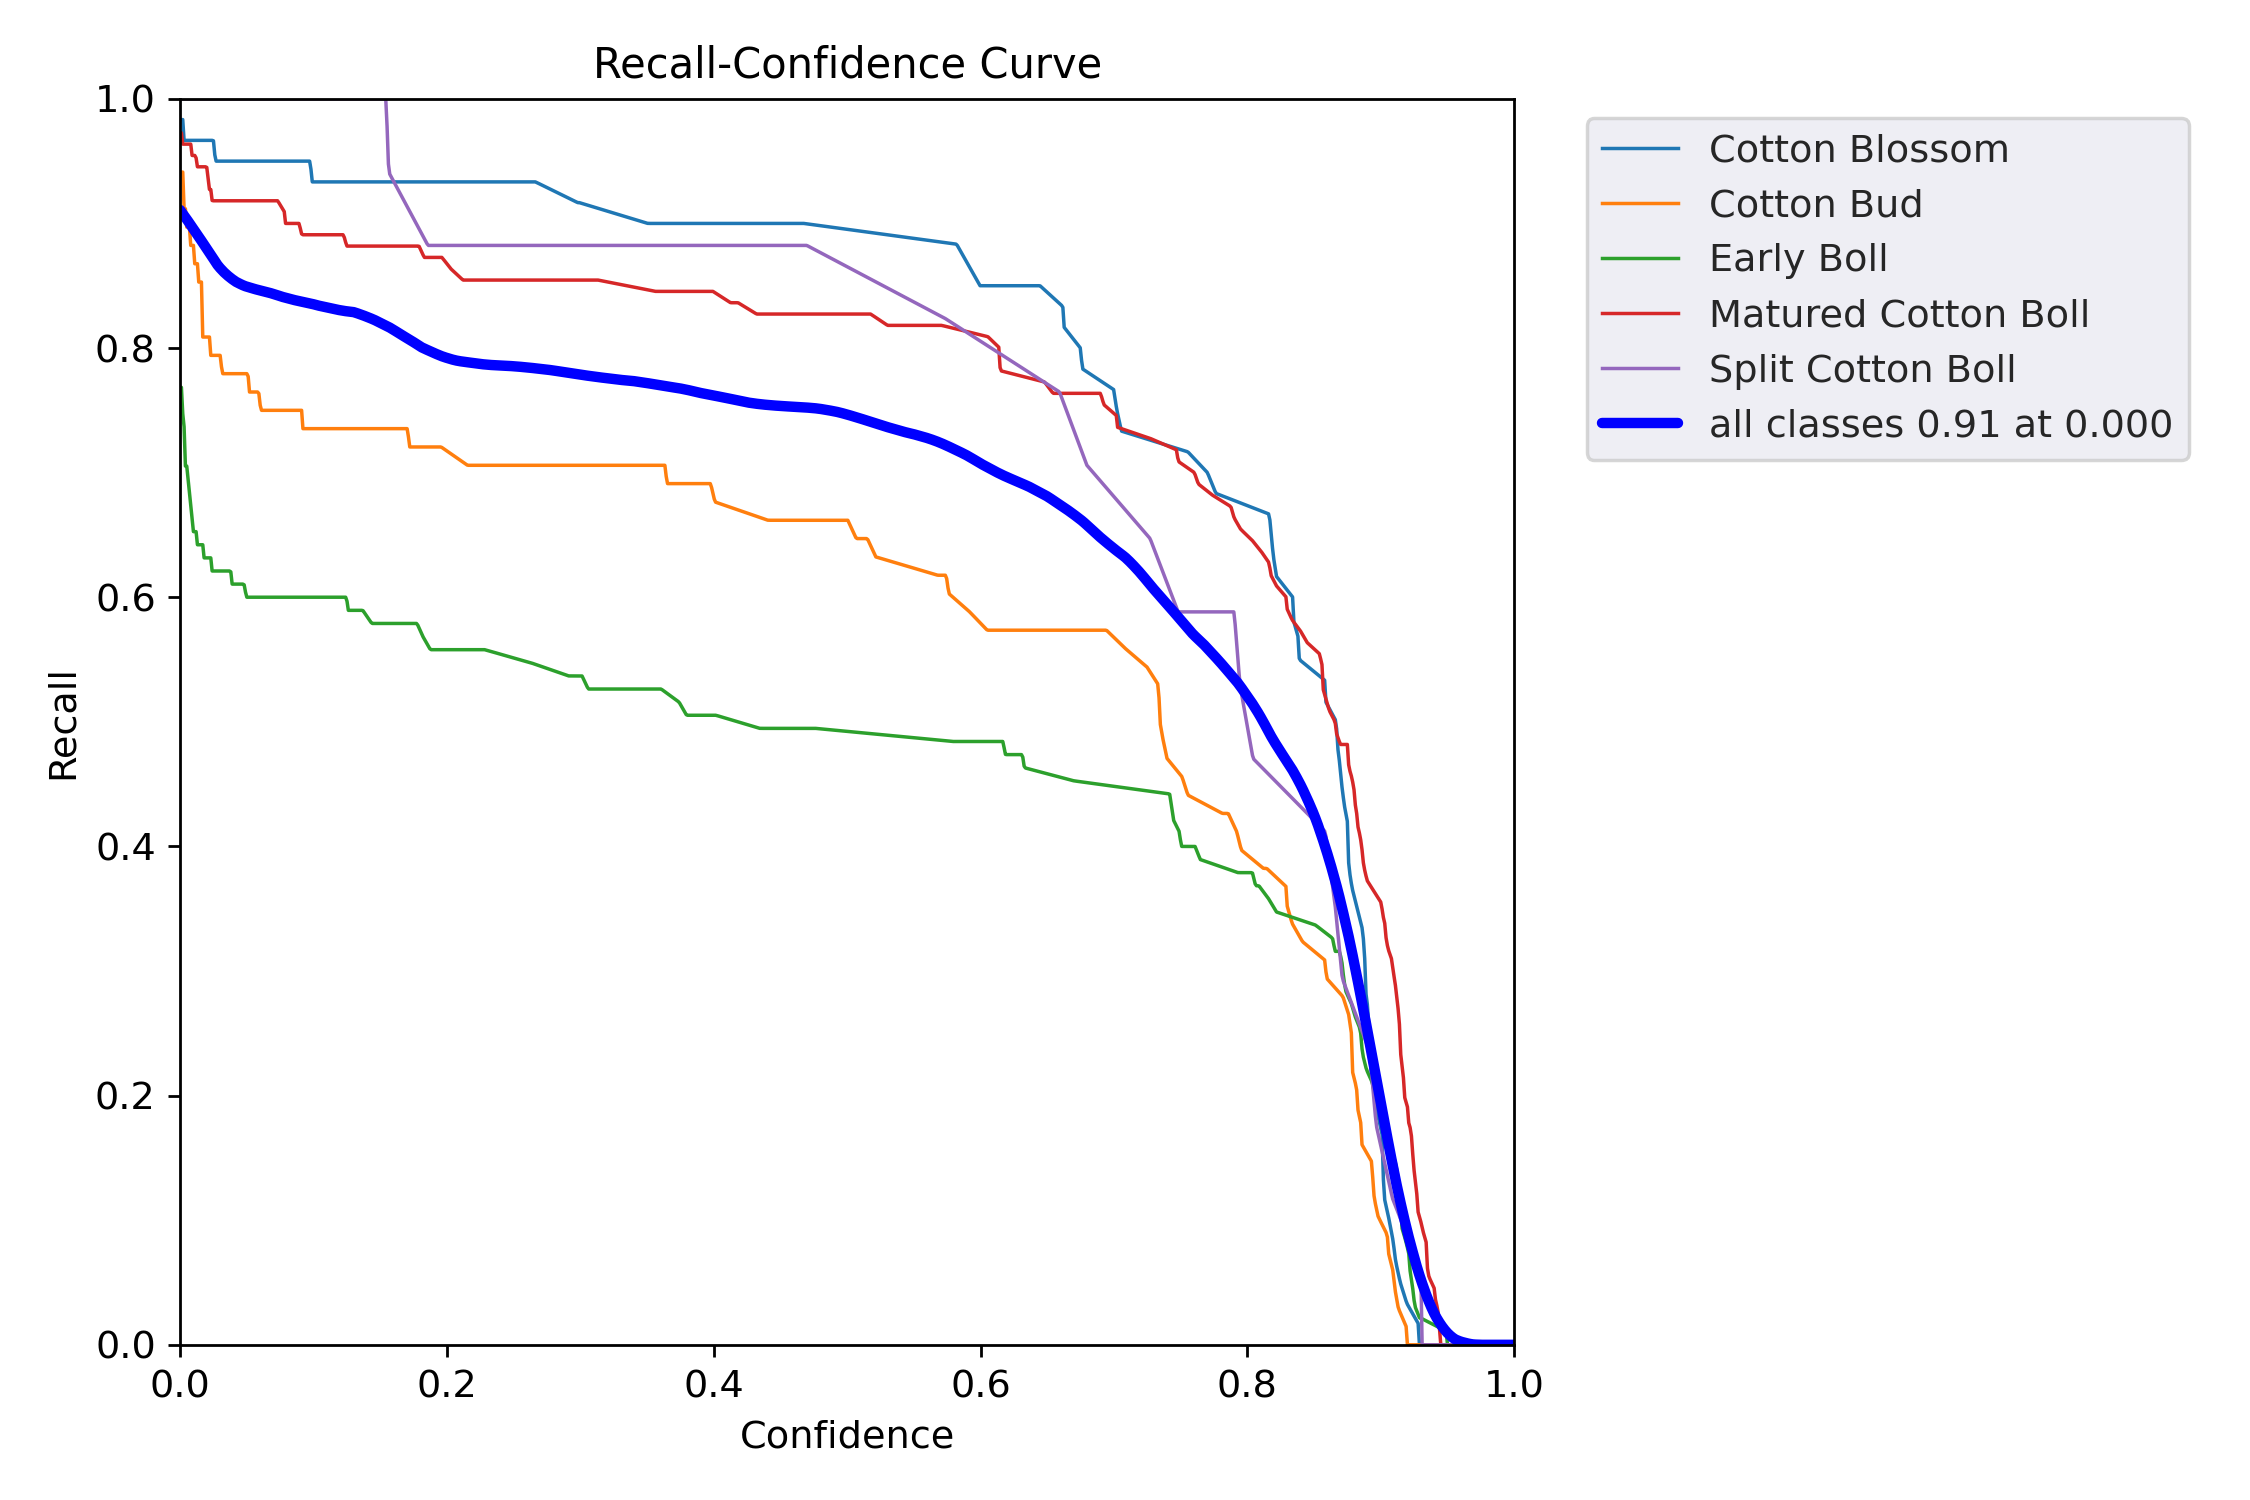
\includegraphics[scale=0.6]{images/results/R_curve.png}
\caption{Recall confidence curve}
\end{center}
\end{figure}

\par Above figure shows the relationship between the trained model's recall and confidence.


\begin{figure}[!htb]
\begin{center}
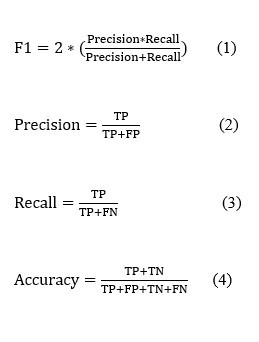
\includegraphics[scale=0.9]{images/results/evaluation metrics.jpg}
\caption{Evaluation metrics}
\end{center}
\end{figure}


\par The summary of performance metrics is given in the following table which gives information of precision, recall and F1 score of multiple classes. 




\begin{table}
\begin{center}
\caption{Performance metrics}% title of Table
\hspace*{0.2in}
\\
\begin{tabular}{| p{3cm} | p{3cm} | p{3cm} | p{3cm} |}
\hline


{\bf{lasses}}             &{\bf{Precision}}                    & {\bf{Recall}}             &{\bf{F-! score}}  \\ \hline
cotton Blossom                  & 0.8                              & 0.93                       & 0.87        \\ \hline
Cotton Bud                      & 0.66                             & 0.71                       & 0.68        \\ \hline
Early Boll                      & 0.67                             & 0.55                       & 0.60        \\ \hline
Mature Cotton               	& 0.77                             & 0.84                       & 0.80        \\ \hline
Split Cotton                    &0.91	                           & 0.87	                    & 0.88 \\ \hline


\end{tabular}
\end{center}
\end{table}



\begin{figure}[!htb]
\begin{center}
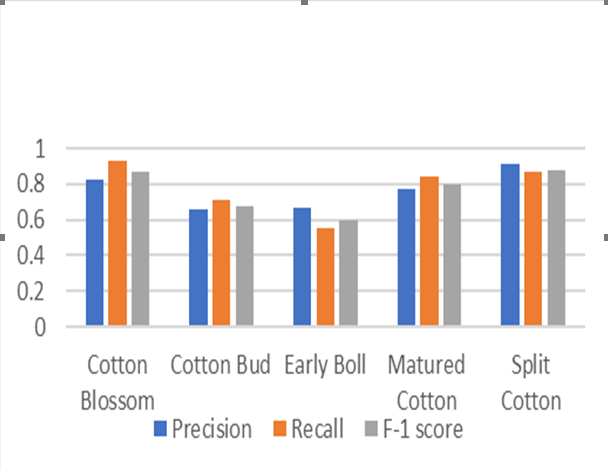
\includegraphics[scale=0.7]{images/results/performance.png}
\caption{Performance metrics}
\end{center}
\end{figure}




\item {\bf{ Hardware Results }} 

\begin{figure}[H]
\begin{center}
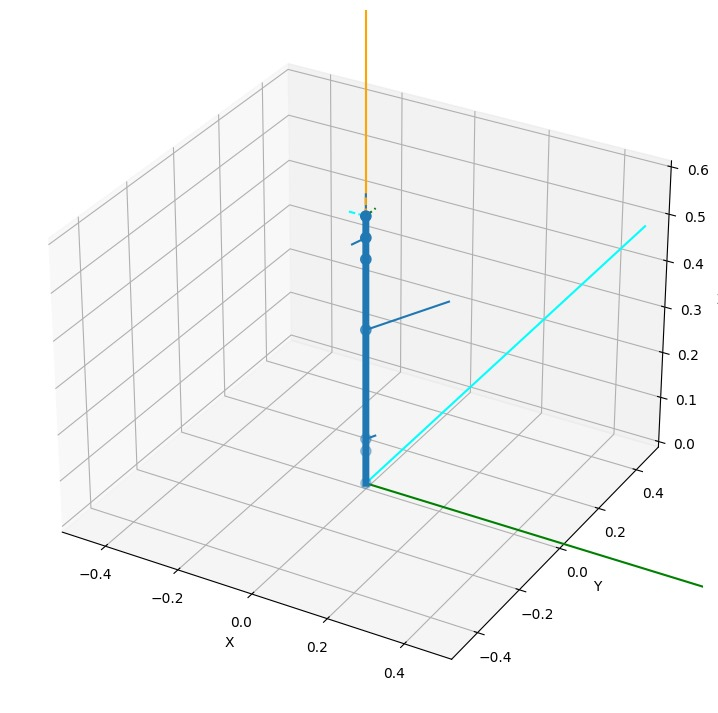
\includegraphics[scale=0.3]{images/results/simulation_1.jpg}
\hspace{0.2in}
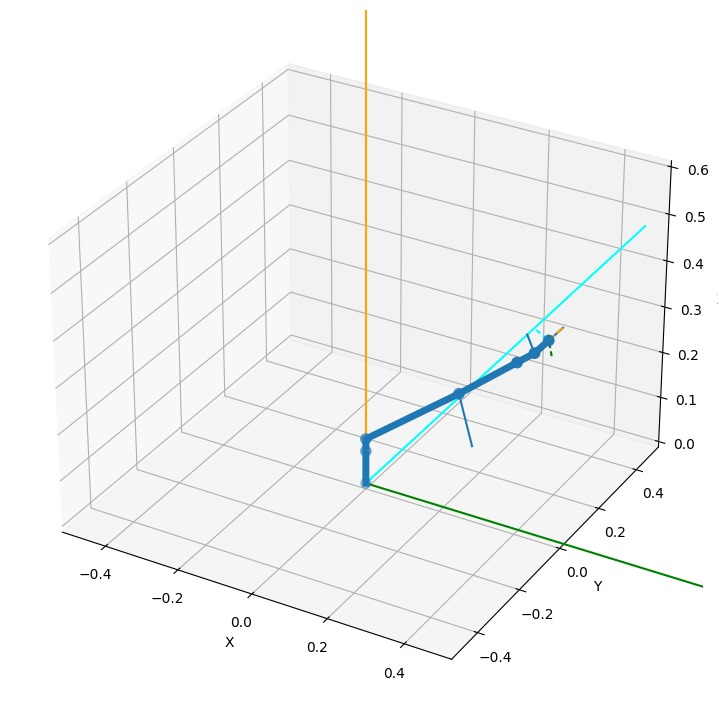
\includegraphics[scale=0.3]{images/results/simulation_2.jpg}
\caption{Simulation results for the position of the robotic arm}
\end{center}
\end{figure}


\par Concerning with the above figure, the simulation results were obtained by running a Python program on Jupyter Notebook which depicted the position of the robotic arm. To get the position and the required angles required for the movement of the arm, the 3d coordinates were provided to the program which then calculates the angles for each joint resulting in the positioning of the end effect-or at the mentioned 3d coordinates to the program.

\begin{figure}[H]
\begin{center}
\includegraphics[scale=0.03]{images/results/real_result_1.jpg}
\hspace{0.2in}
\includegraphics[scale=0.03]{images/results/real_result_2.jpg}
\caption{Results of working of the robotic arm}
\end{center}
\end{figure}

\par 
The Python code that developed the simulation results was modified into Embedded C for real-time servos control and uploaded on Arduino Mega. The micro controller was able to actuate the servos according to the coordinates provided, based on the calculation of the angles for each joint the simulation results and the real-time working of the arm had similar results. The model is shown in above figure.














\end{enumerate} 


\newpage




\section {Summary}

\par The summary of the report is to create a reliable system that can recognize, handle, harvest, and transport cotton blooms.

\par A rover equipped with a robot arm and a storage area for processed cotton blooms would be the ideal setup for that.

\par The system's overall practical application is to decrease the amount of labor and resources needed for cotton harvesting while increasing its profitability and efficiency.
%%%%%%%%%%%%%%%%%%%%%%%%%%%%%%%%%%%%%%%%%%%%%%%%%%%%%%%%%%%%%%%%%%%%%


\chapter{Advantage and Applications}


\section{Advantages}
The advantages of the proposed system can be summarized as follow:
\begin{enumerate}
\item There is no need for human intervention as the robot can work autonomously.
\item Real-time image processing improves crop yield and making the process more
efficient.
\item Improved accuracy of cotton detection and chances of missing or damaging the
cotton is less.
\item Using computer vision the probability of unripe cotton being harvested is less,
thereby ensuring minimal wastage.
\item Reducing need for chemical defoliation, machine learning based detection
contributes to environment friendly practices.

\end{enumerate}
\section{Applications}
the proposed system can be employed at variety of applications such as :
\begin{enumerate}
\item Crop yield estimation
\item Textile industry
\item Disease and pest detection
\end{enumerate}
%%%%%%%%%%%%%%%%%%%%%%%%%%%%%%%%%%%%%%%%%%%%%%%%%%%%

%%%%%%%%%%%%%%%%
\chapter{ Conclusion and Future Scope}


\section {Conclusion}

\par   In this paper, an object detection technique called YOLOv5 (You Only Look Once version 5) was used to construct a model for cotton detection. With the help of YOLOv5 and a PyTorch-compatible dataset, we successfully developed and trained a cotton recognition model using the Google Colab platform. In order to teach the model to recognize and correctly anticipate the existence of cotton bolls in new, unseen photos, annotated photographs of cotton bolls at different stages of growth were fed to it. The cotton bloom, cotton bud, early boll, matured boll, and split cotton boll are the five different categories into which the cotton detection model was intended to identify and categorize cotton bolls. Following the training phase, the model showed a high degree of accuracy in identifying and categorizing these various cotton boll phases. 




\begin{figure}[H]
\begin{center}
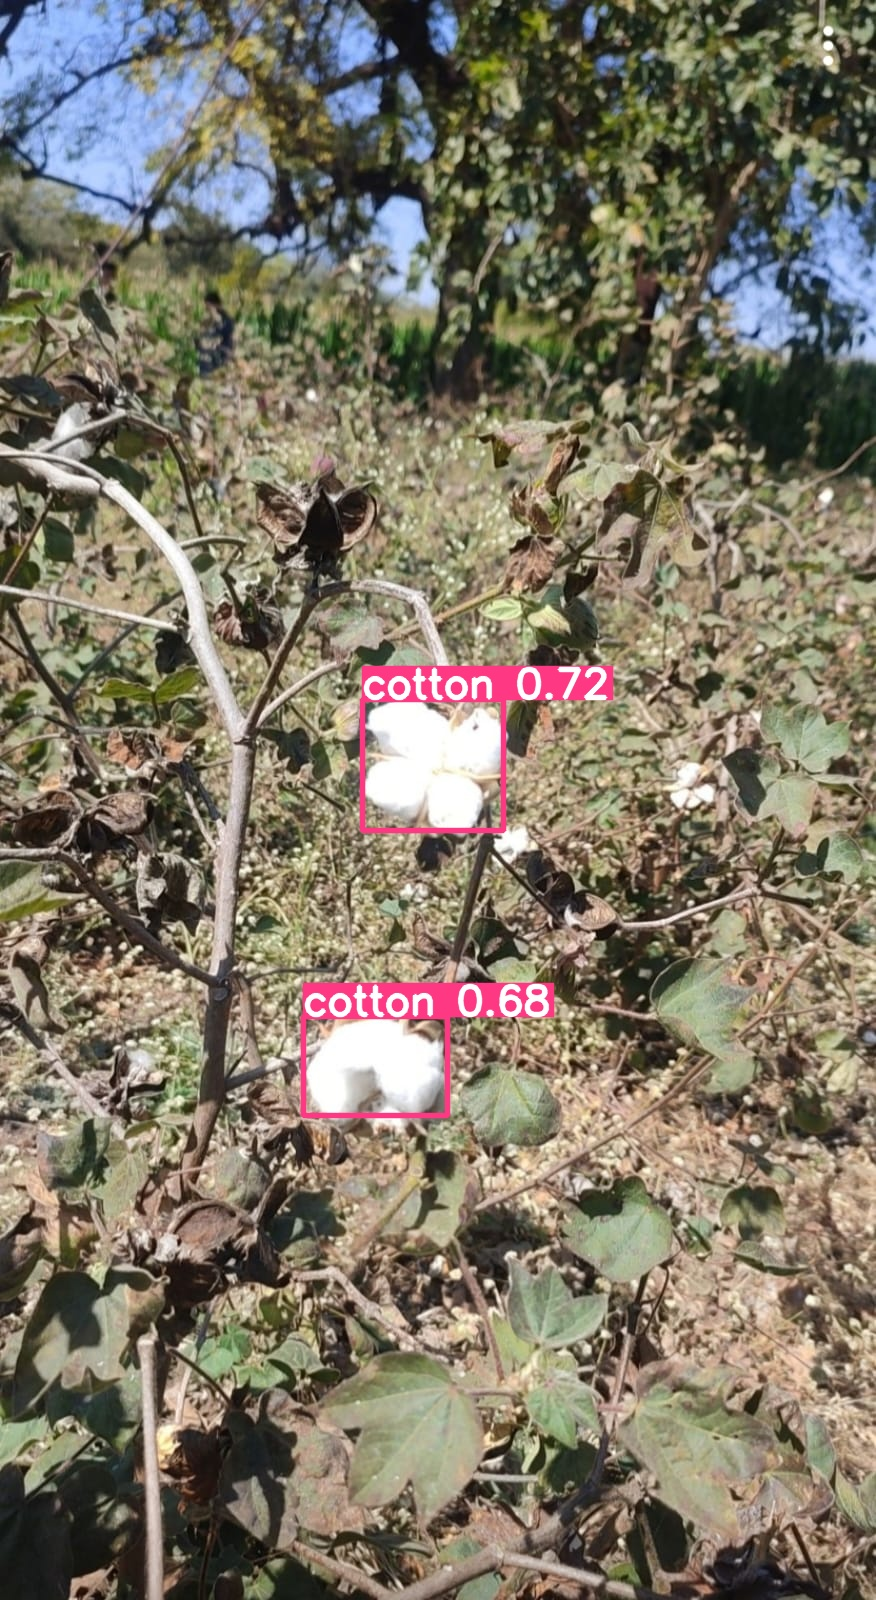
\includegraphics[scale=0.2]{images/results/7.jpg.jpg}
\hspace{0.2in}
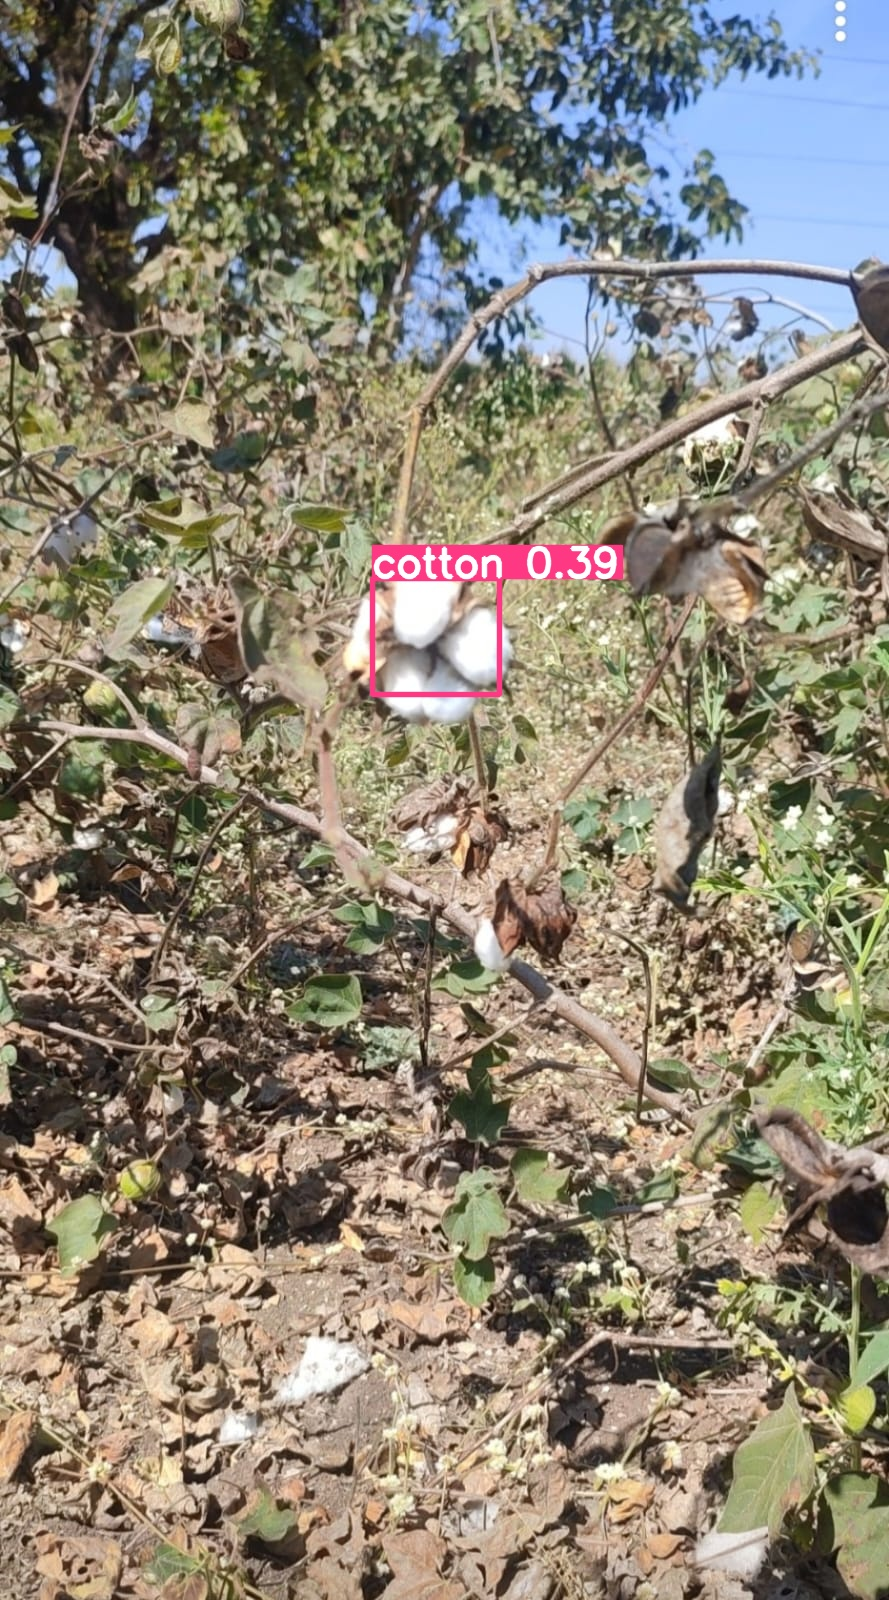
\includegraphics[scale=0.2]{images/results/9.jpg.jpg}
\caption{Real time testing of model using Images}
\end{center}
\end{figure}






\par Regarding the robotic arm, while it was intended to reach specific locations and execute picking operations using determined angles, it was not feasible to incorporate the cotton detecting model within the parameters of this project. Nonetheless, simulation of the robotic arm's functionality was done, and the results demonstrated that the arm could precisely locate given coordinates and carry out picking tasks as predicted. The simulation results matched the theoretical requirements closely and showed promise. In order to establish a seamless and autonomous cotton-picking system, future work will concentrate on fully integrating the robotic arm with the YOLOv5-based cotton detecting algorithm. By lowering labor costs and raising productivity in the cotton sector, this integration hopes to open the door for more sophisticated agricultural robots solutions.


\newpage

\section {Future Scope}

\begin{enumerate}

   \item {\bf{Combining Various Sensor Systems:}}
Use a range of sensors, including LiDAR and infrared sensors, to provide the robot with a thorough grasp of the surroundings in the cotton field.
   \item {\bf{Personalized Path Planning and \\ Self-governing Navigation:}}
To improve the robot's agility in the field, create complex algorithms for autonomous navigation and dynamic path planning.
   \item {\bf{Technological Developments in Image Processing:}}
Investigate and apply state-of-the-art image processing techniques to improve cotton bloom detection accuracy and speed.
   \item {\bf{Diverse Methods of Harvesting:}}
Consider various cotton plant varieties and field variations while researching and implementing solutions that adapt to changing harvesting conditions.
   \item {\bf{Human-Robot Synchronization:}}
This can entail building interfaces for remote observation and management or allowing the robot to work in control of humans on more complex jobs. 
%    \item {\bf{Capabilities for Multiple Tasks:}}
% To optimize the robot's usefulness in the field, this adaptability may encompass weed detection, soil analysis, or other tasks.
%    \item {\bf{Features for Human Safety:}}
% These could include adding sensors and algorithms that let the robot recognize and react to people or animals.
%    \item {\bf{Global Navigation System Integration: }}
% To increase accuracy and position awareness, this may entail integrating GPS or other satellite-based navigation technology.

\end{enumerate}





\bibliographystyle{ieeetr} 
\bibliography{mybib1}

%%%%%%%%%%%%%%%%%%%%%%%%%%%%%%%%%%%%%%%%%%%%

%\end{thebibliography}
%%%%%%%%%%%%%%%%%%%%%%%%%%%%%%%%%%%%%%%%%%%%%%%%%%%%%%%%%%
%\begin{thebibliography}{99}
%\bibitem{}http://latex-project.org/
%\bibitem{}Android Wireless Application Development Guide  by Shane Conder
%\bibitem{and}www.android.com
%\bibitem{w}http://en.wikipedia.org/wiki/Android(operating system)
%\end{thebibliography}
%
\appendix
% \appendixpage
% \noappendicestocpagenum

\chapter{Project Outcomes}%This is just for showing, where it shows up, in my original, it says only Appendix here.

\section {Plagiarism Report}
\includegraphics[scale =0.4]{images/plagiarism/plag1.jpeg}
\newpage
\includegraphics[scale=0.4]{images/plagiarism/plag2.jpeg}
\newpage
\includegraphics[scale =0.4]{{images/plagiarism/plag3.jpeg}}
\newpage
\includegraphics[scale =0.4]{images/plagiarism/plag4.jpeg}
\newpage
\includegraphics[scale=0.4]{images/plagiarism/plag5.jpeg}
\newpage

\section {Project Competition Participation Certificates}

\begin{figure}[!htb]
\begin{center}
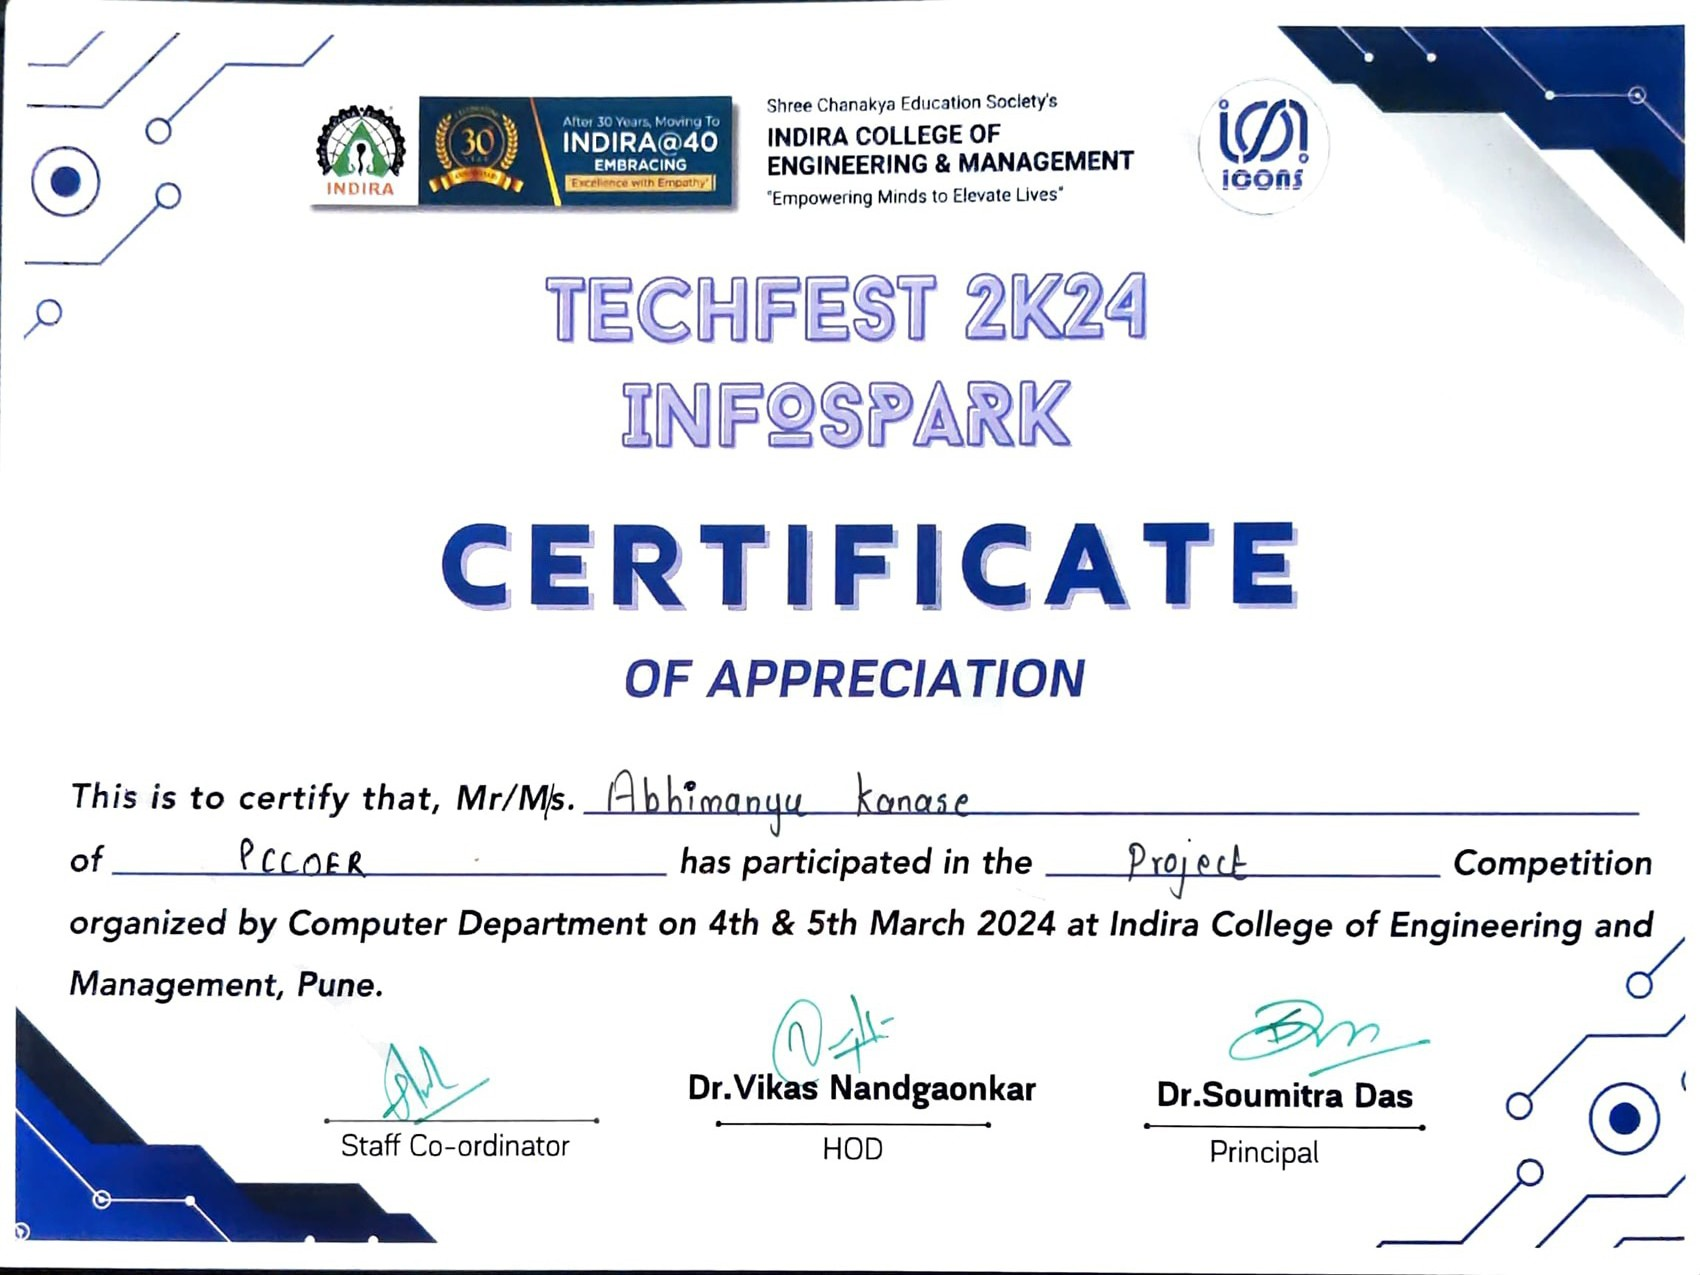
\includegraphics[scale=0.2]{images/certificates/certificates/Abhi1.jpg}
\end{center}
\end{figure}
\begin{figure}[!htb]
\begin{center}
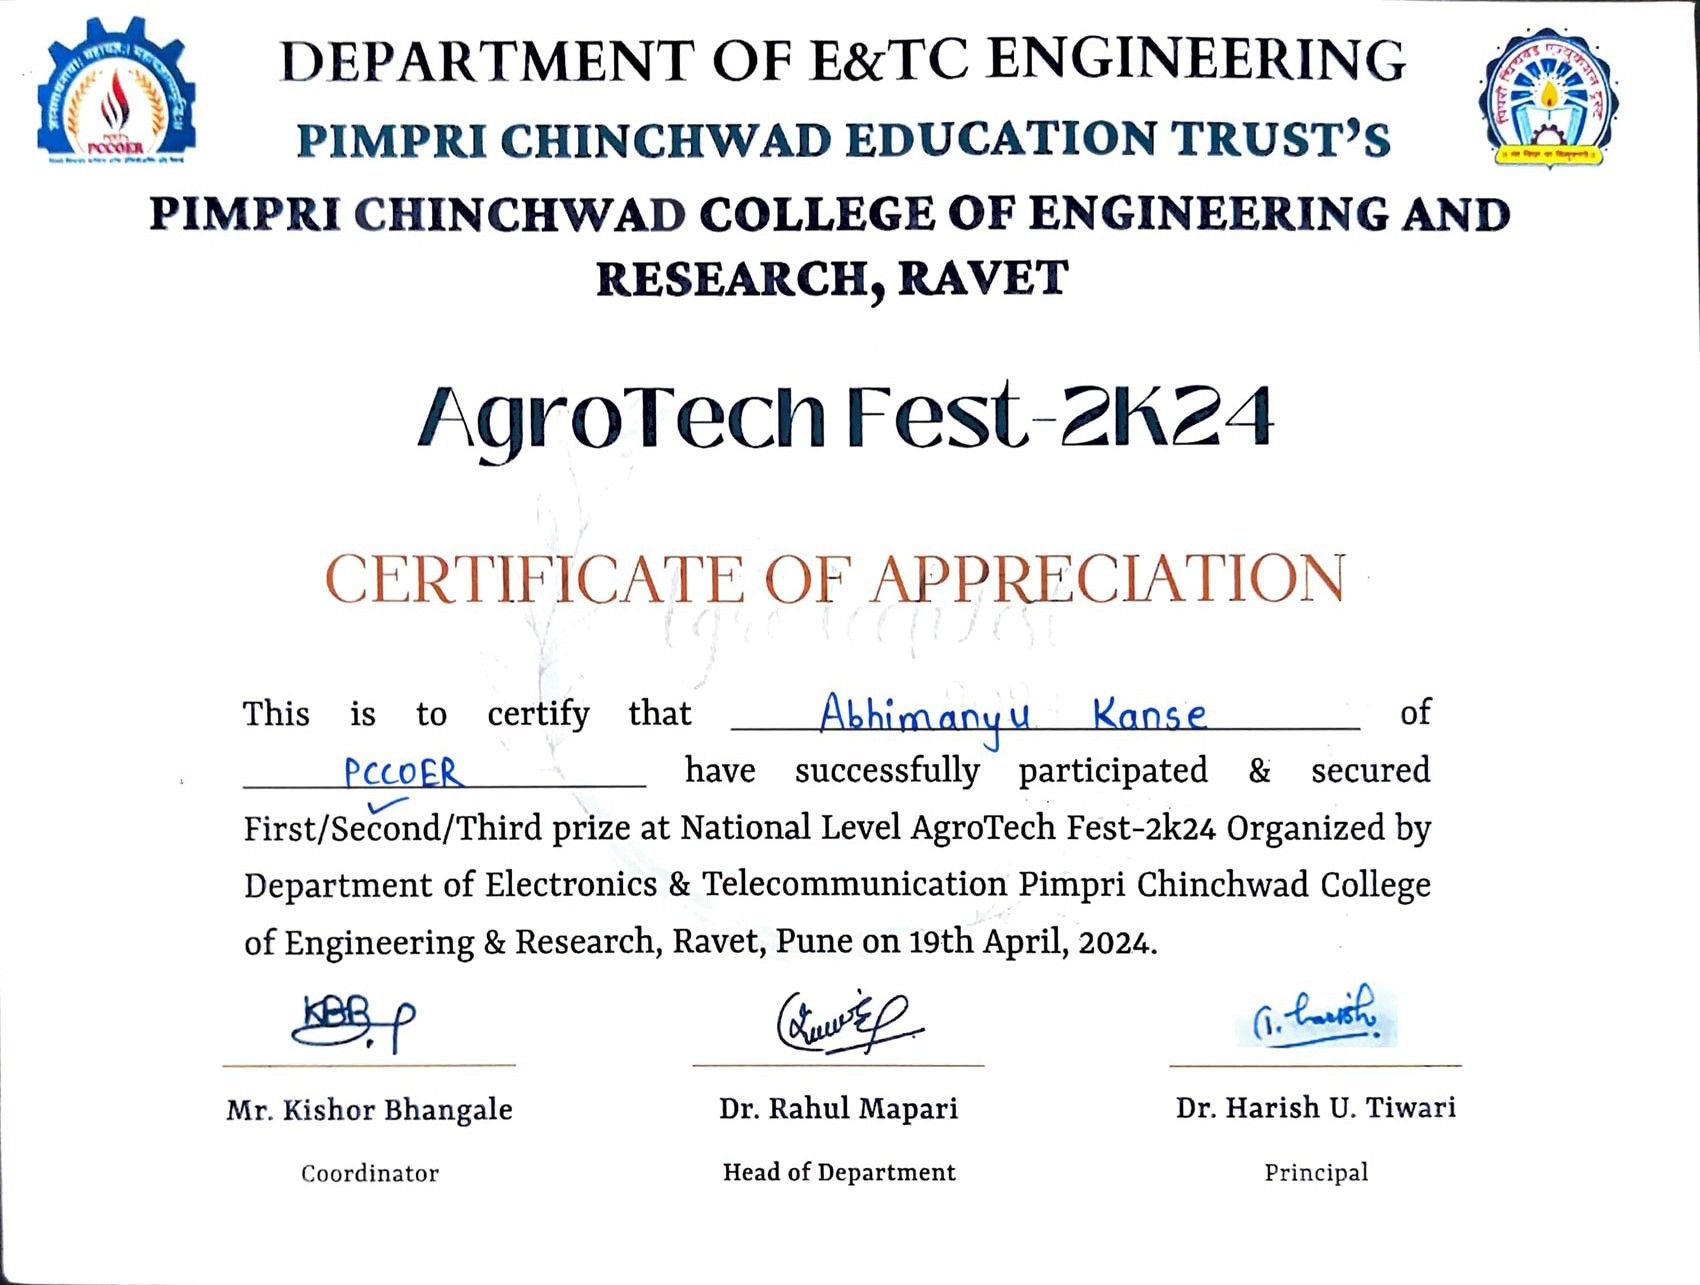
\includegraphics[scale=0.2]{images/certificates/certificates/Abhi2.jpg}
\end{center}
\end{figure}
\begin{figure}[!htb]
\begin{center}
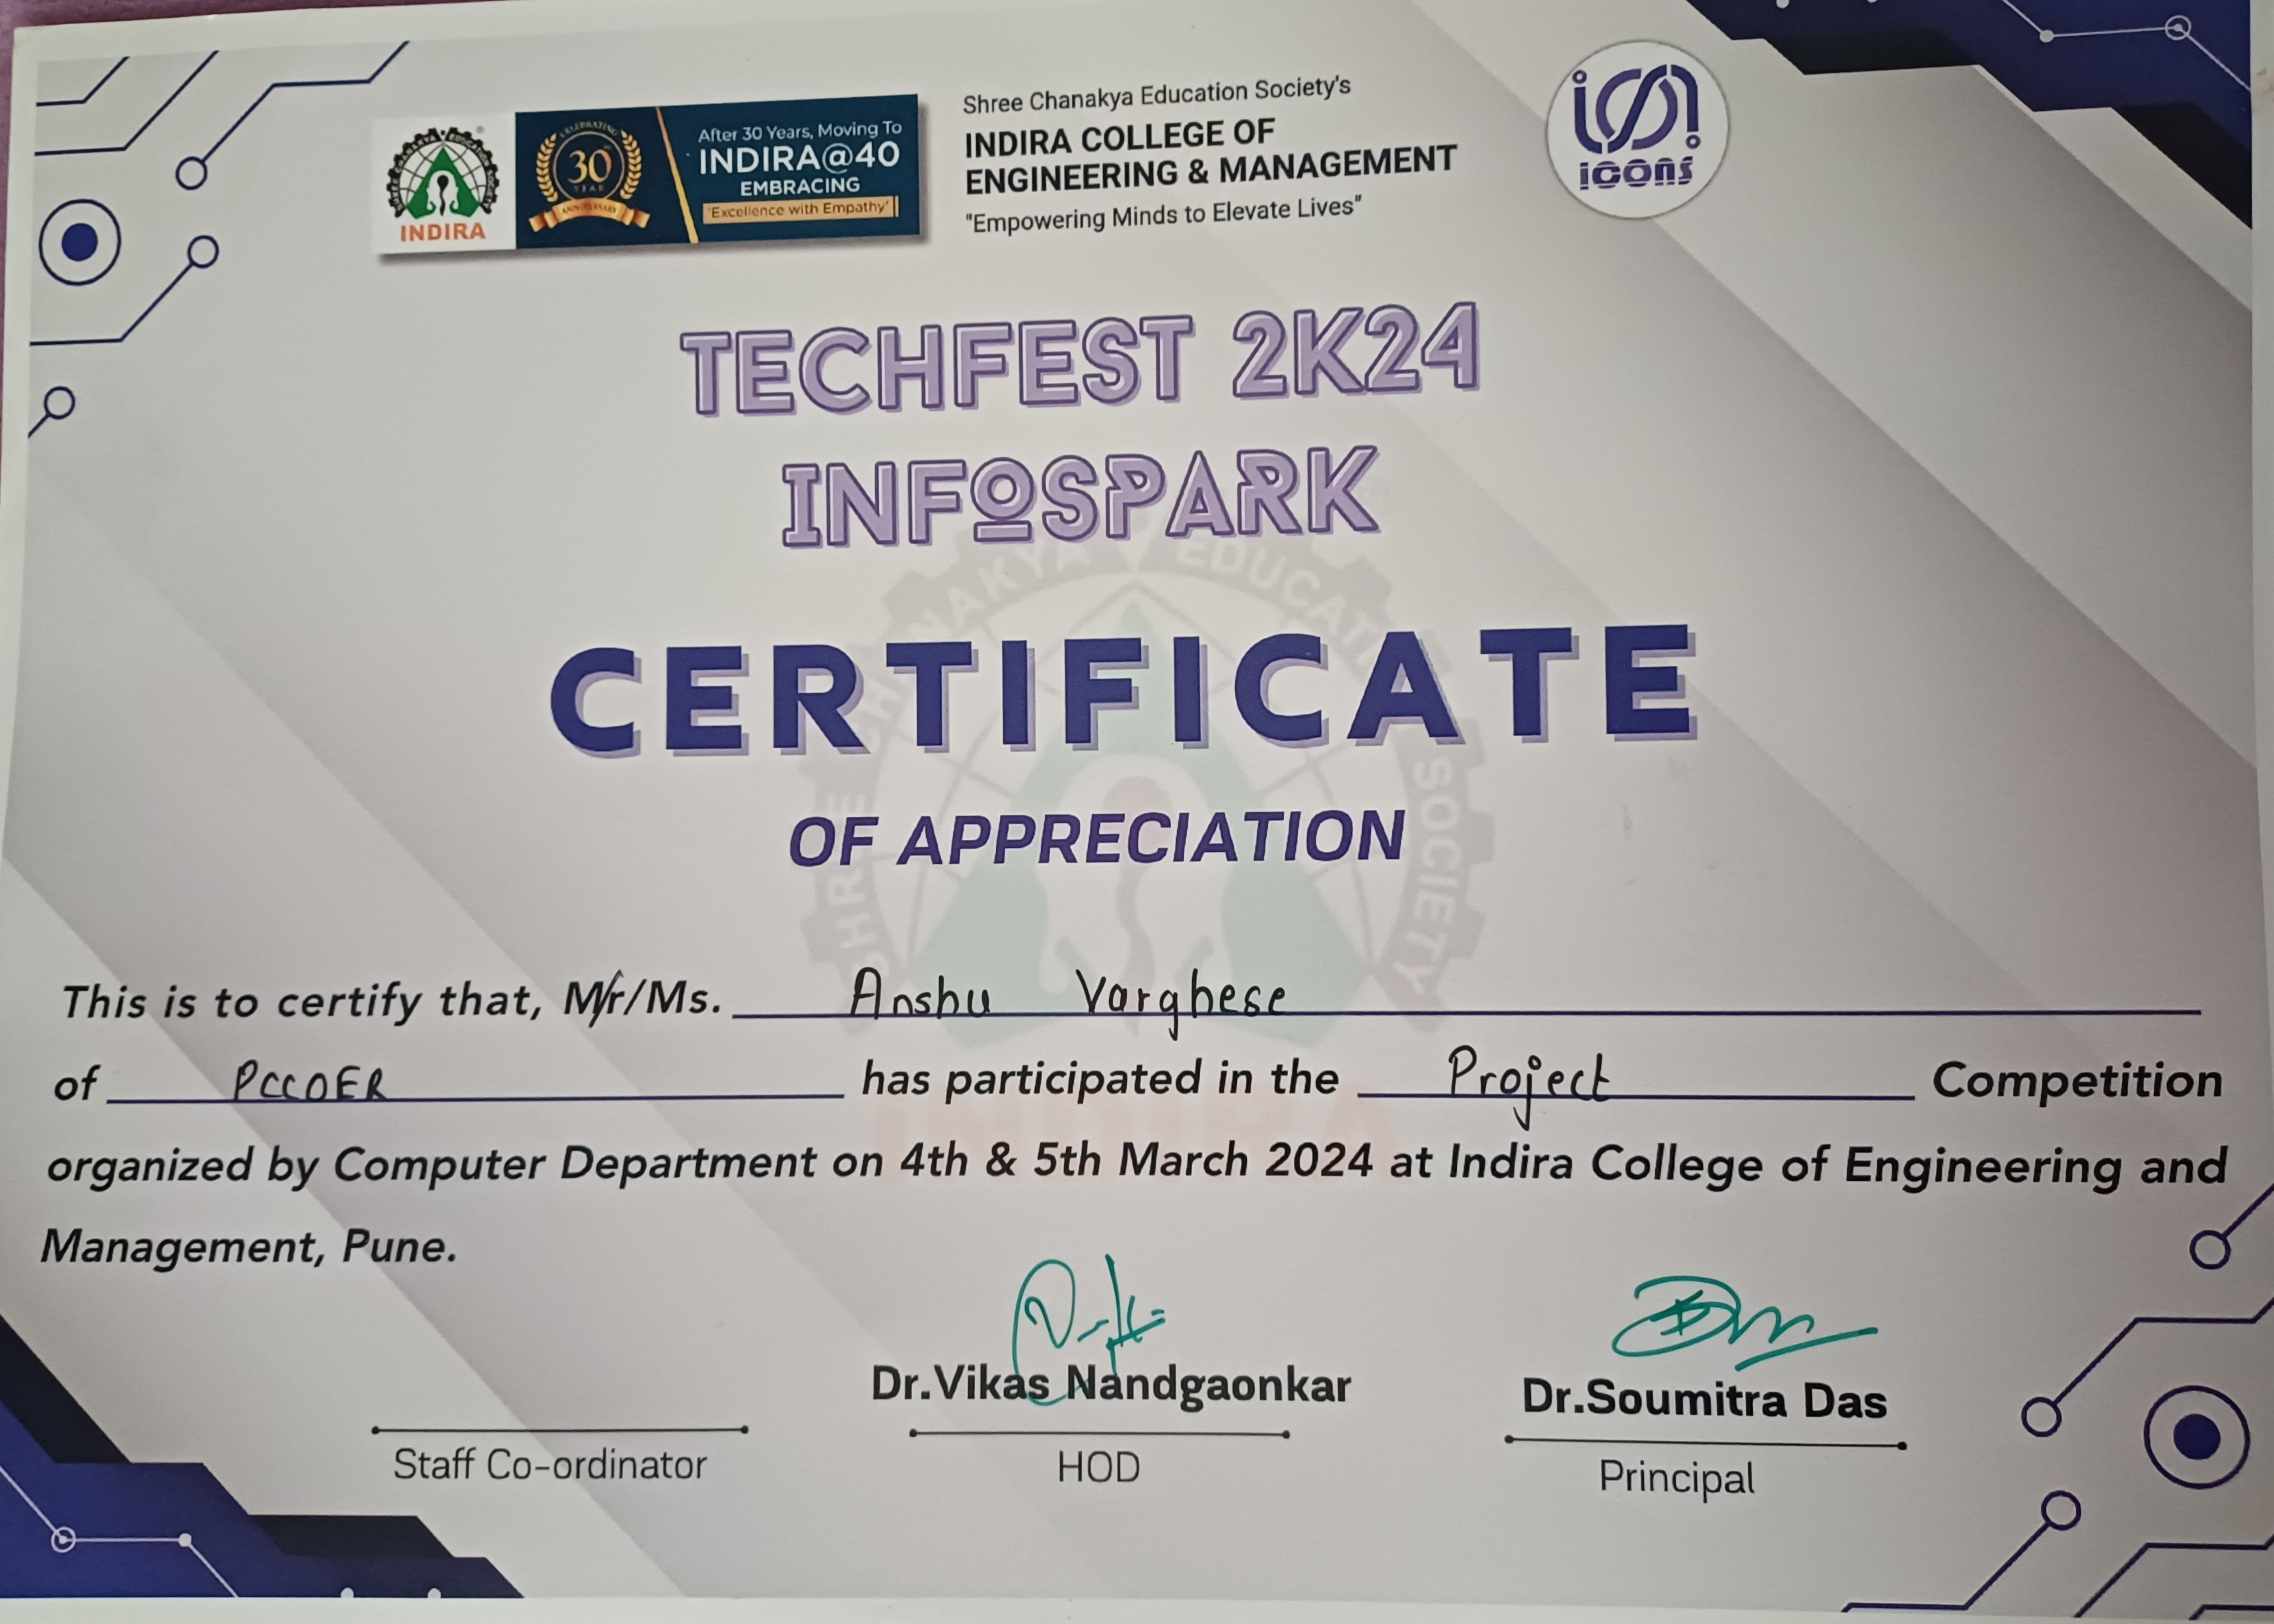
\includegraphics[scale=0.1]{images/certificates/certificates/Anshu1.jpg}
\end{center}
\end{figure}
\begin{figure}[!htb]
\begin{center}
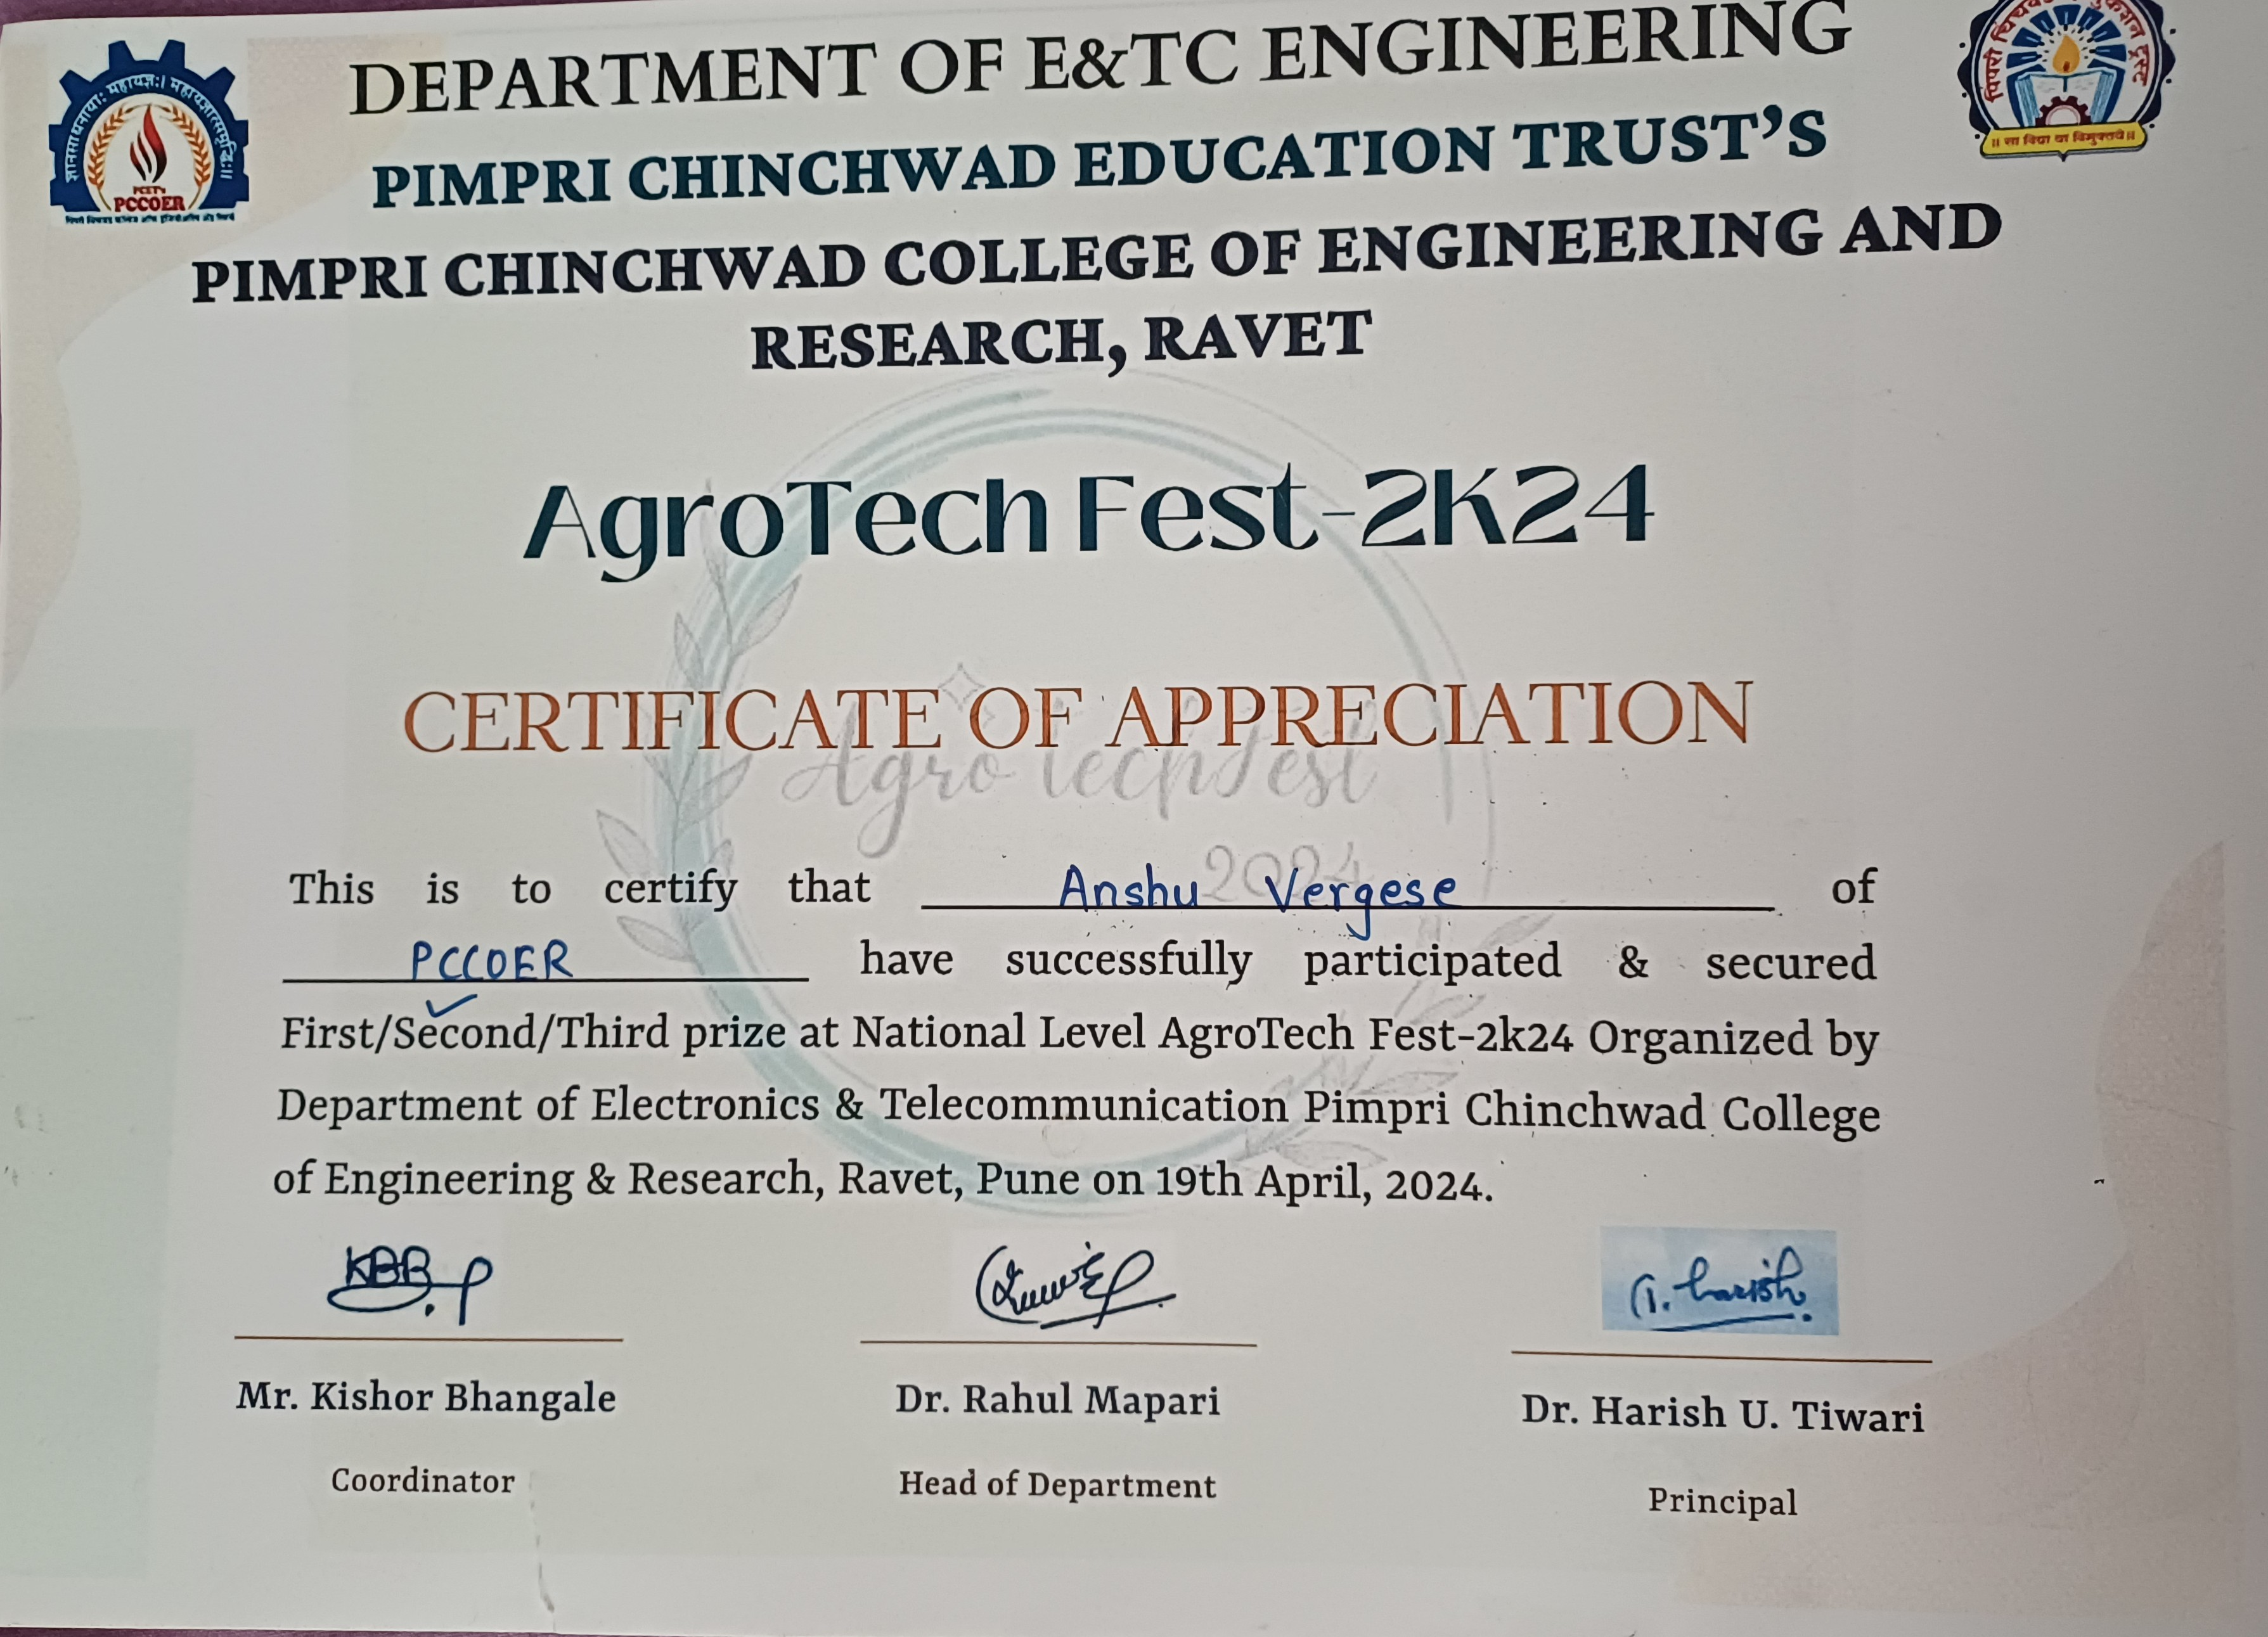
\includegraphics[scale=0.1]{images/certificates/certificates/Anshu2.jpg}
\end{center}
\end{figure}
\newpage
\begin{figure}[!htb]
\begin{center}
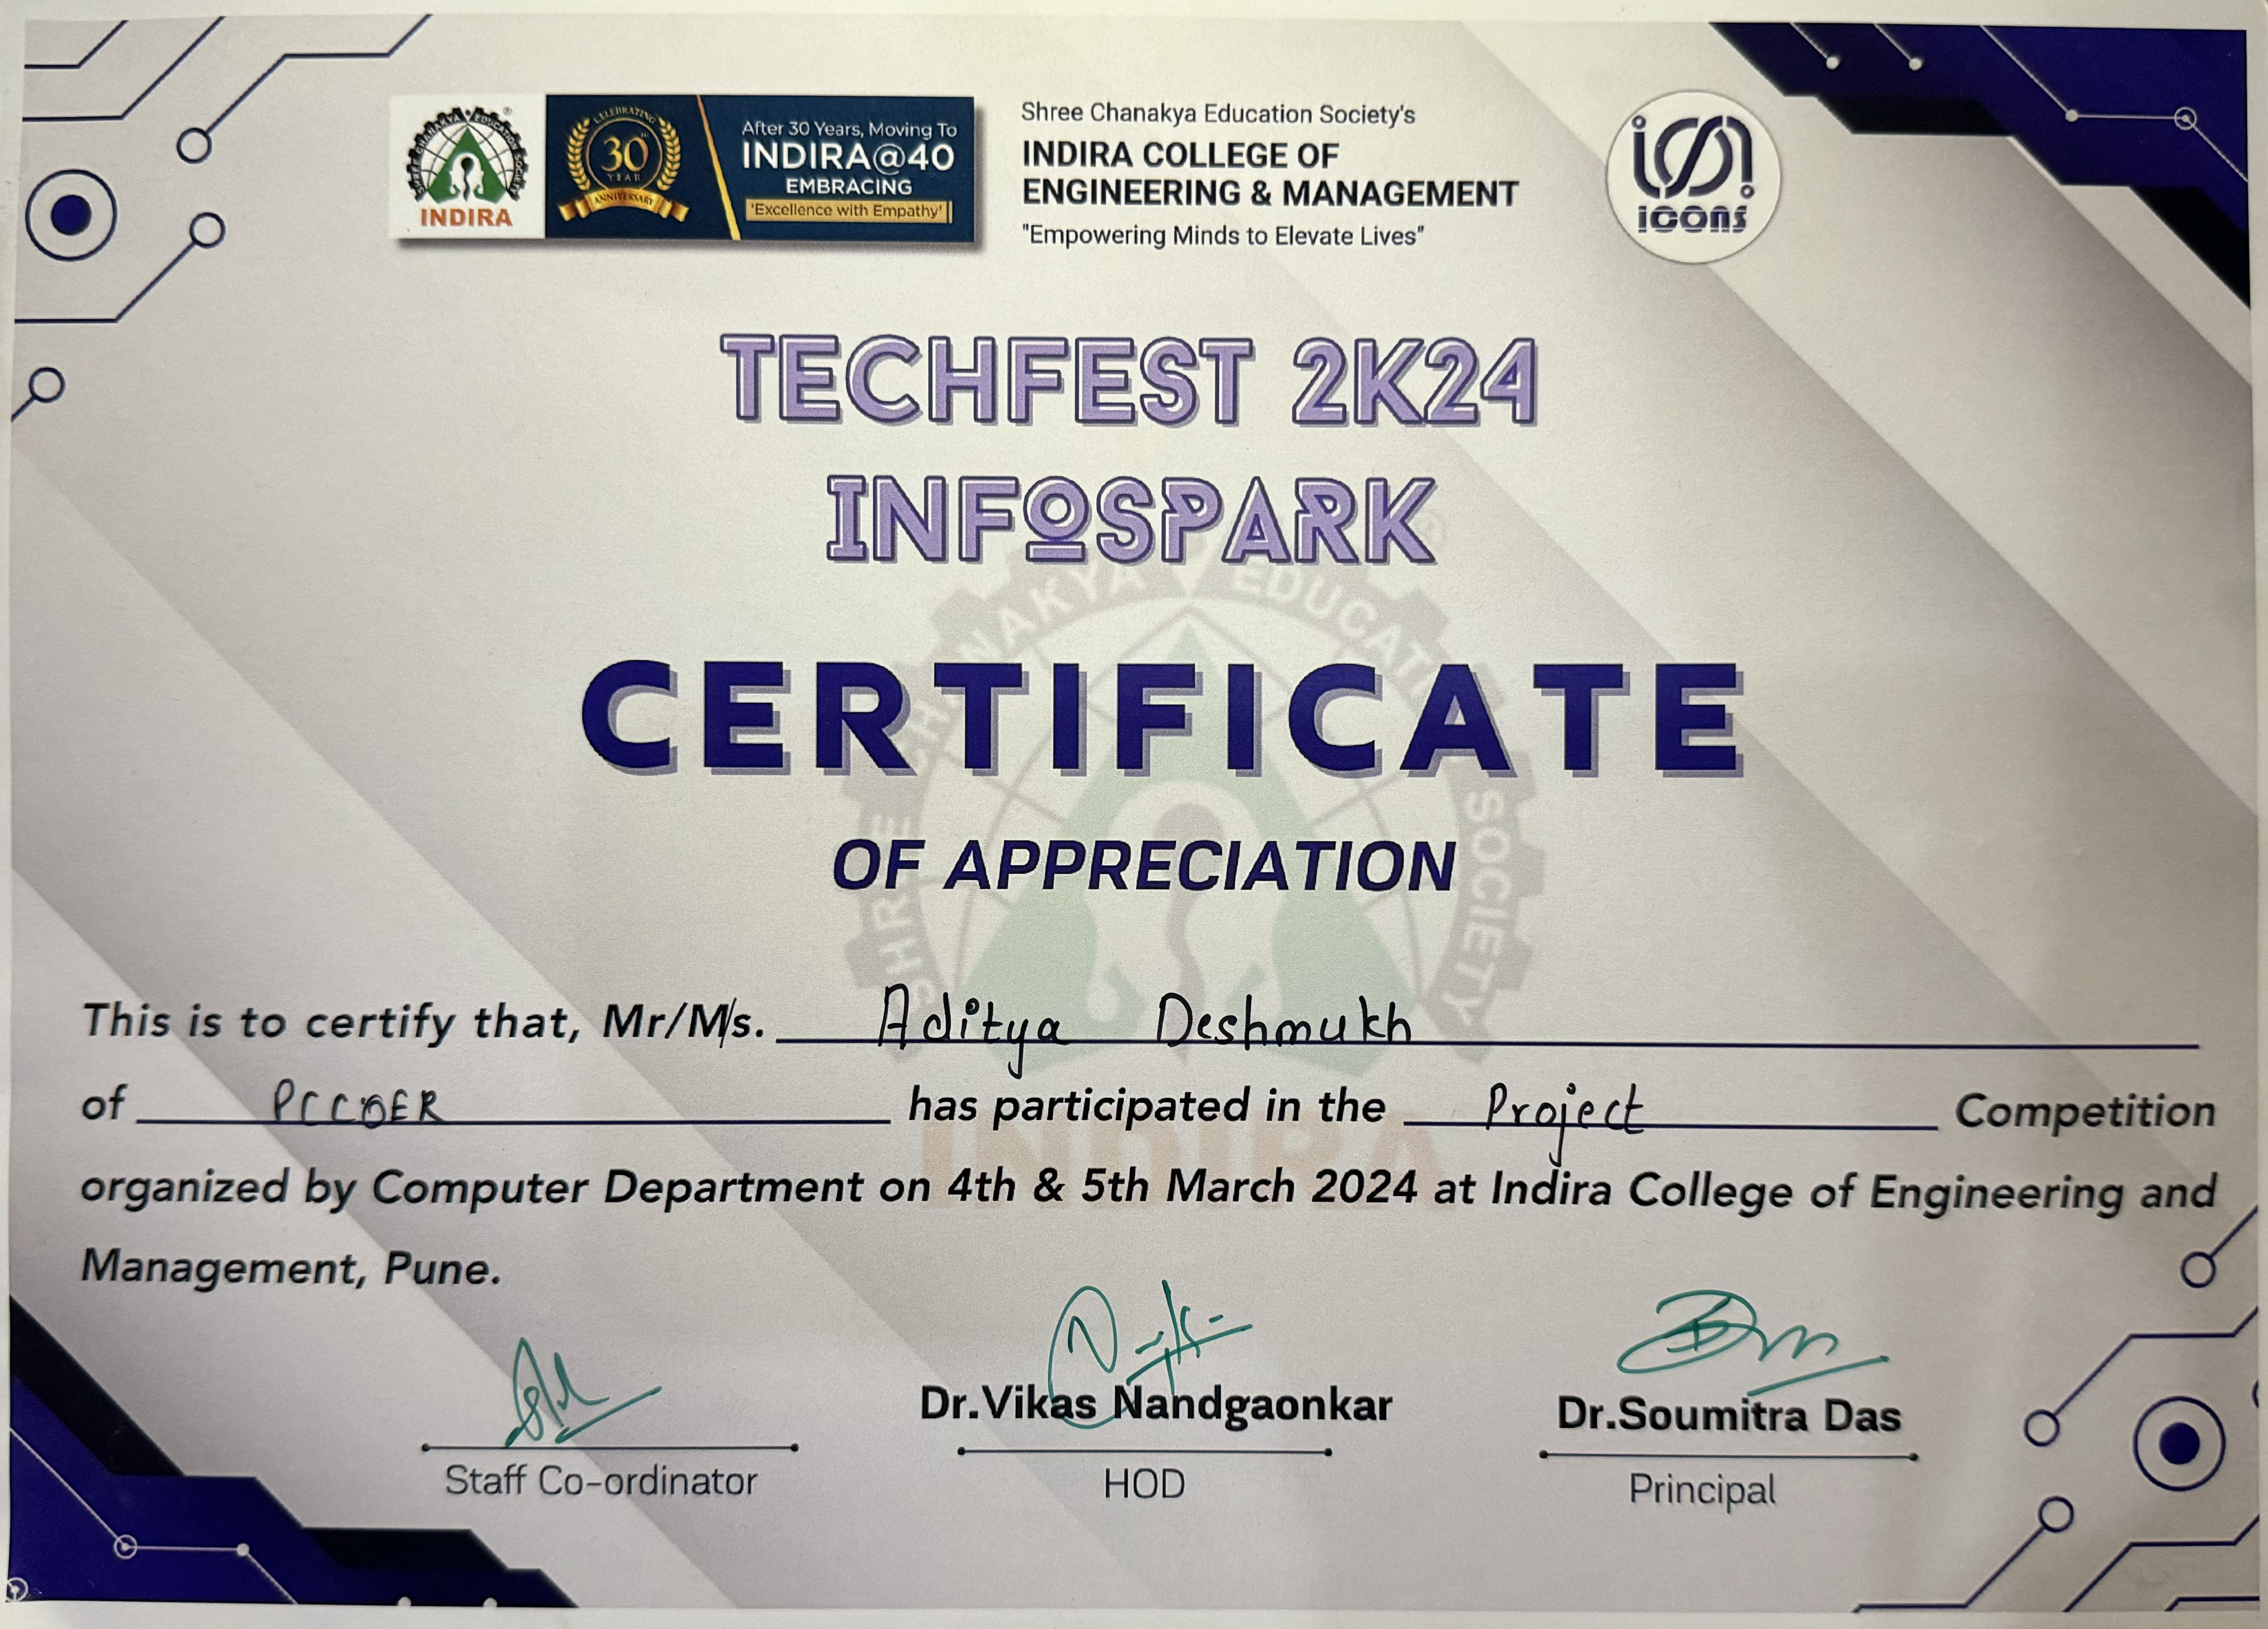
\includegraphics[scale=0.095]{images/certificates/certificates/Aditya1.jpg}
\end{center}
\end{figure}
\begin{figure}[!htb]
\begin{center}
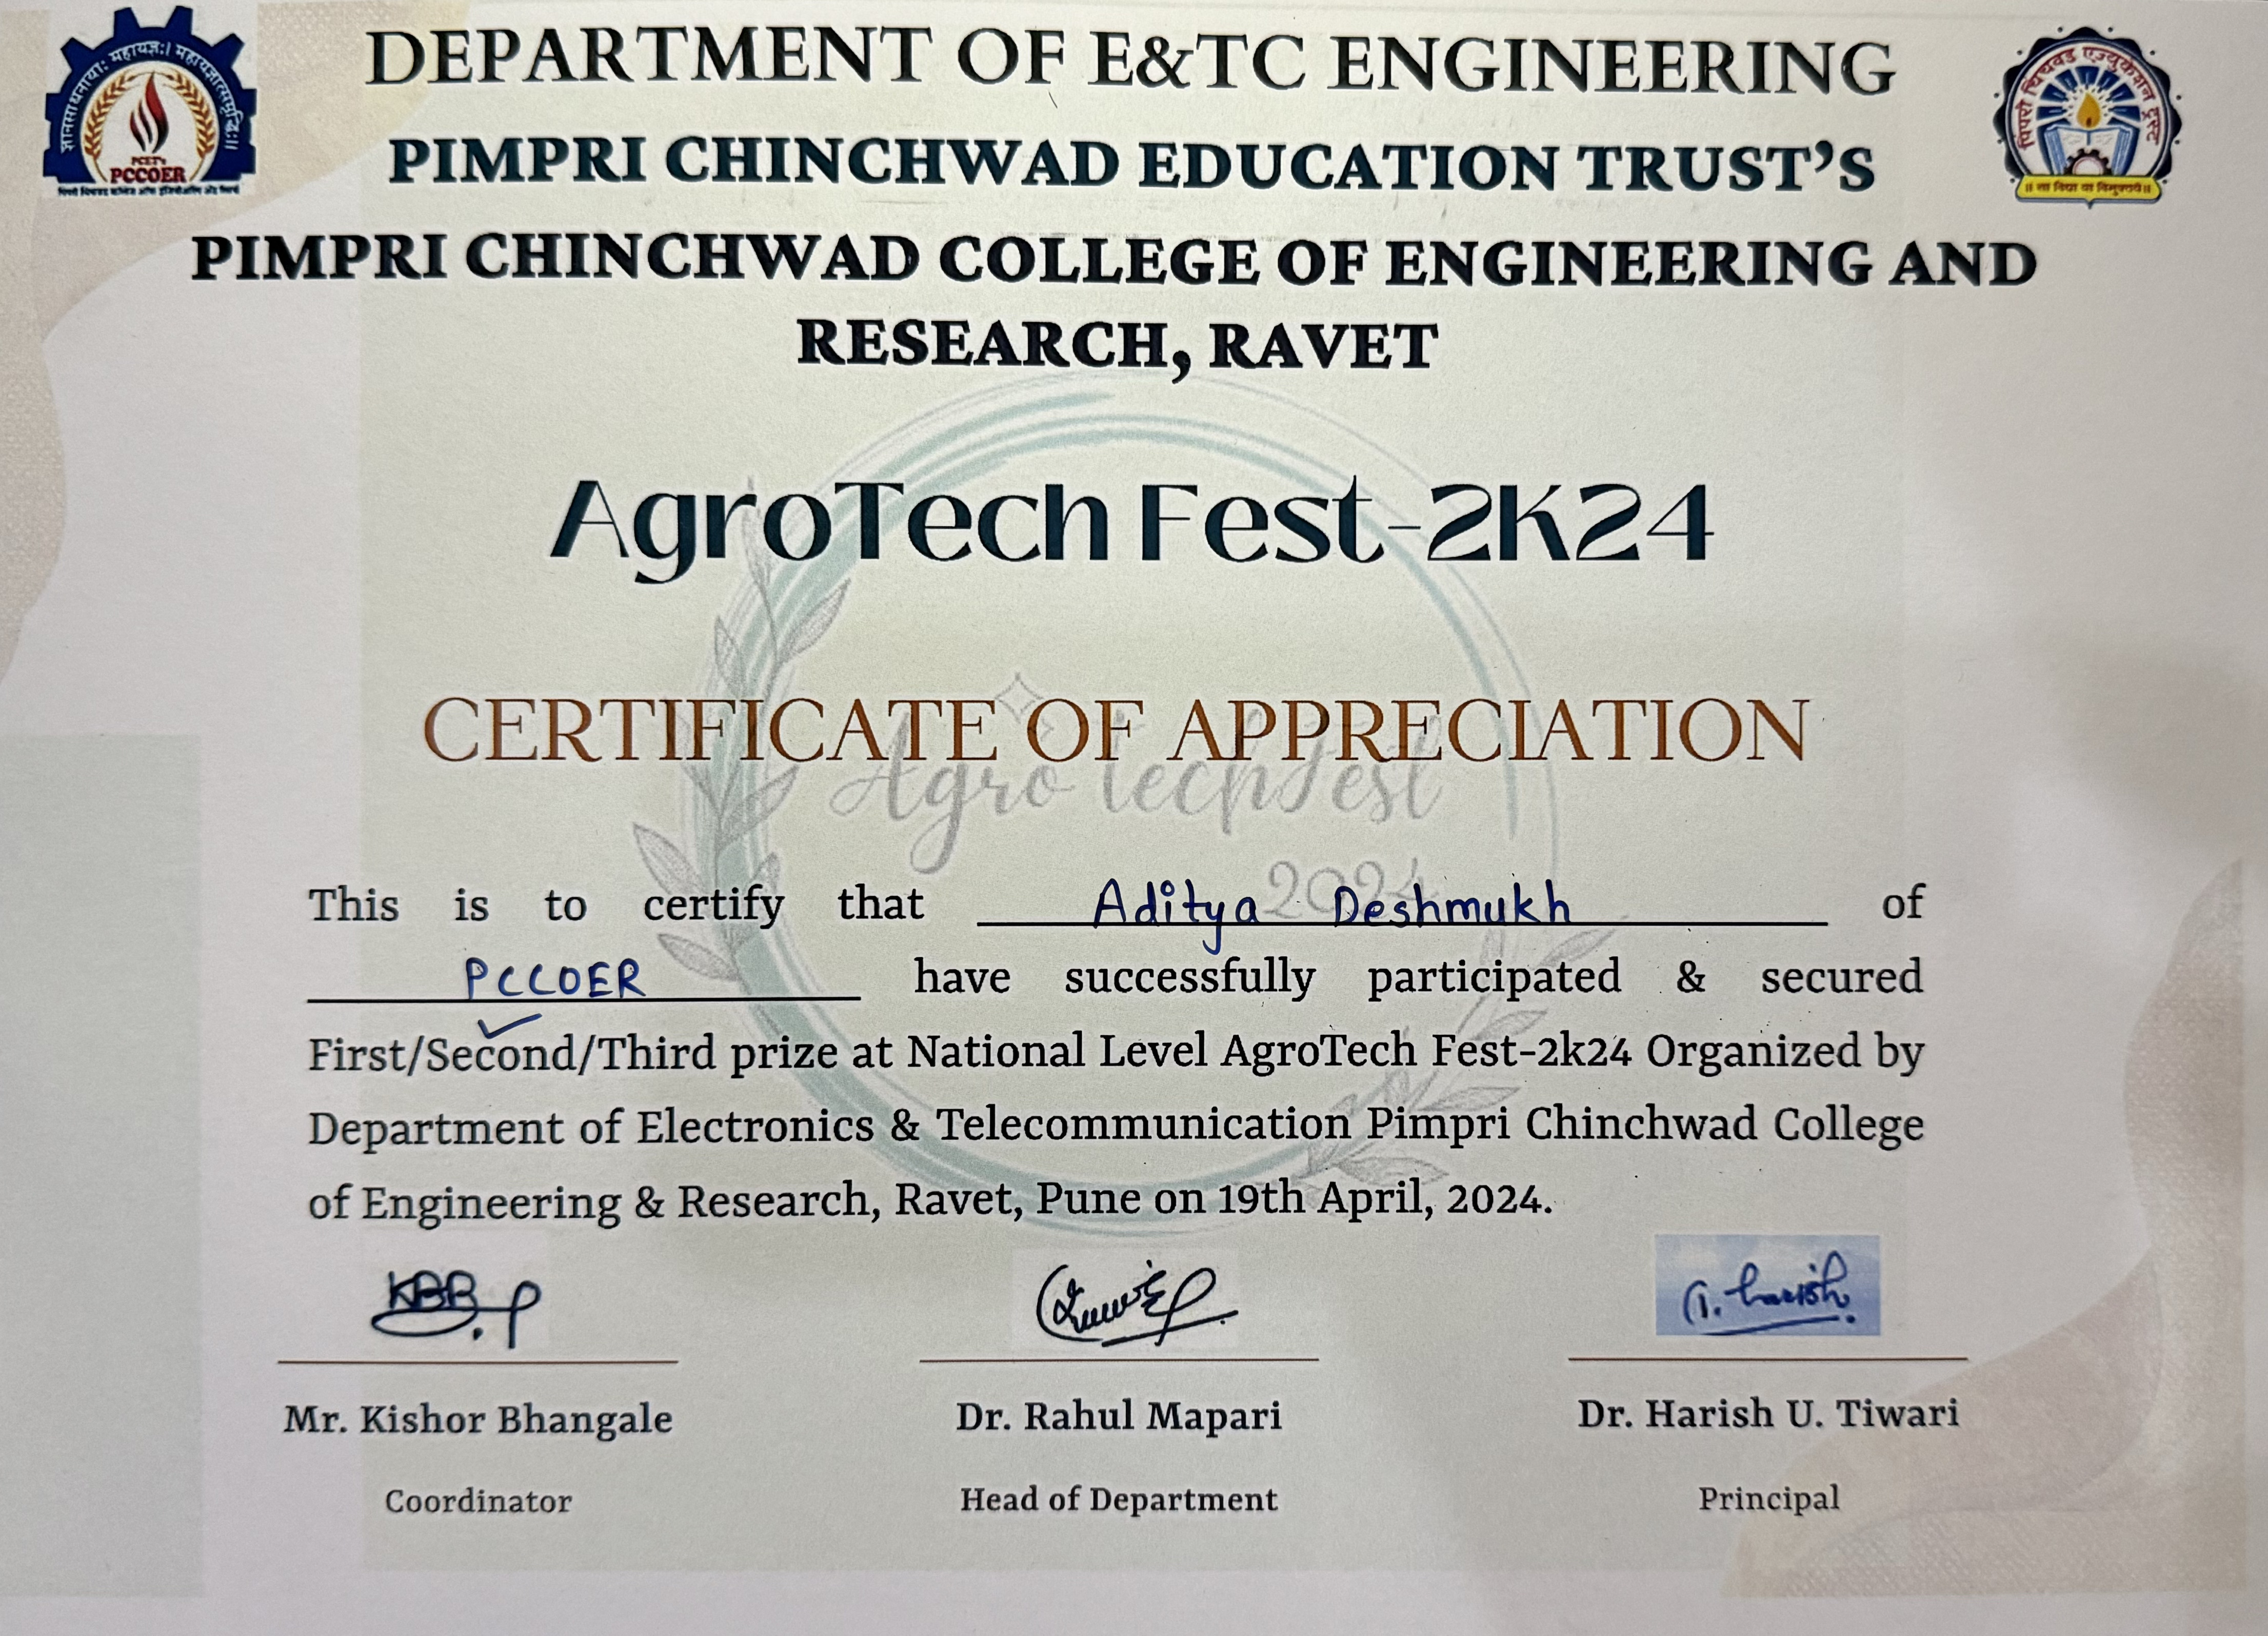
\includegraphics[scale=0.095]{images/certificates/certificates/Aditya2.jpg}
\end{center}
\end{figure}    
\newpage

\section {Publication Documents}
\subsection {Publication Work}
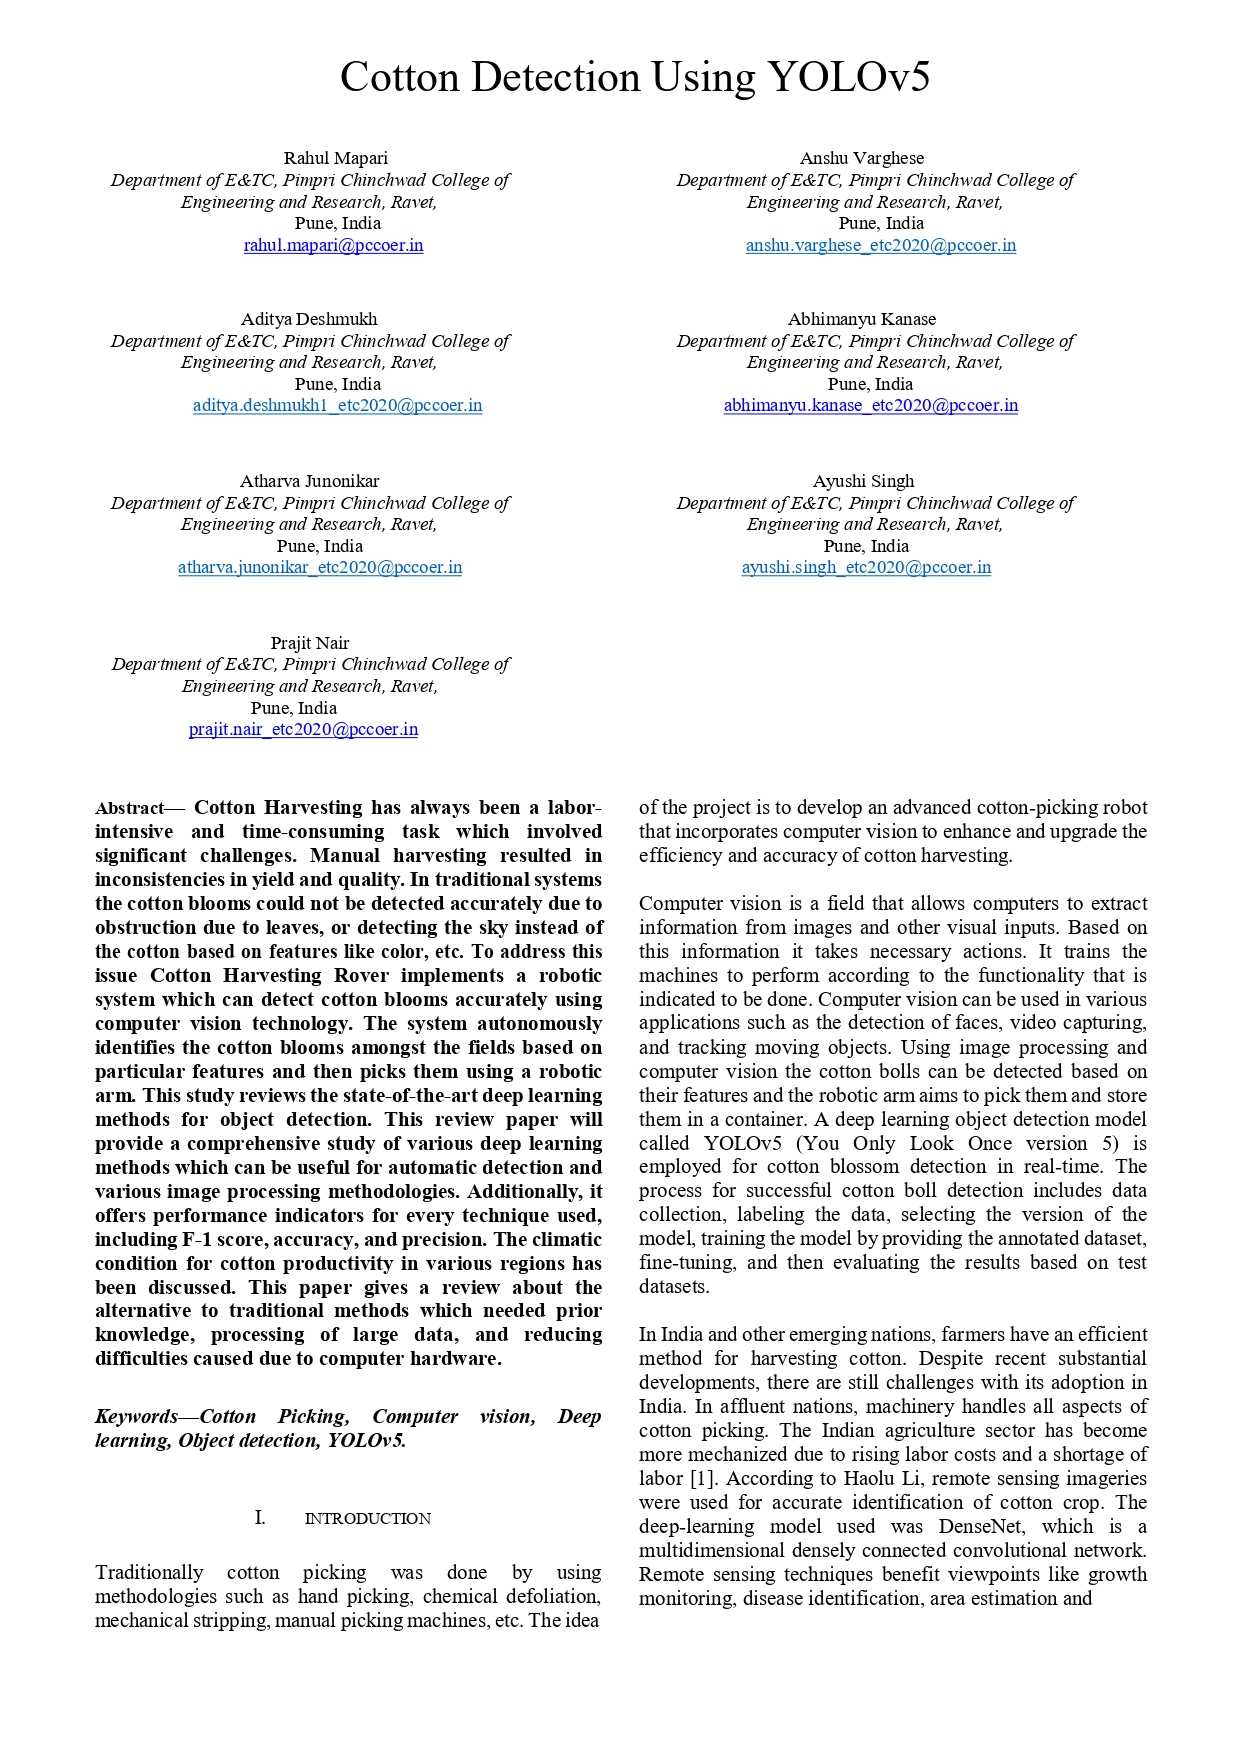
\includegraphics[scale =0.7]{images/copyright/publication/Publication/Publication_page-0001.jpg}
\newpage
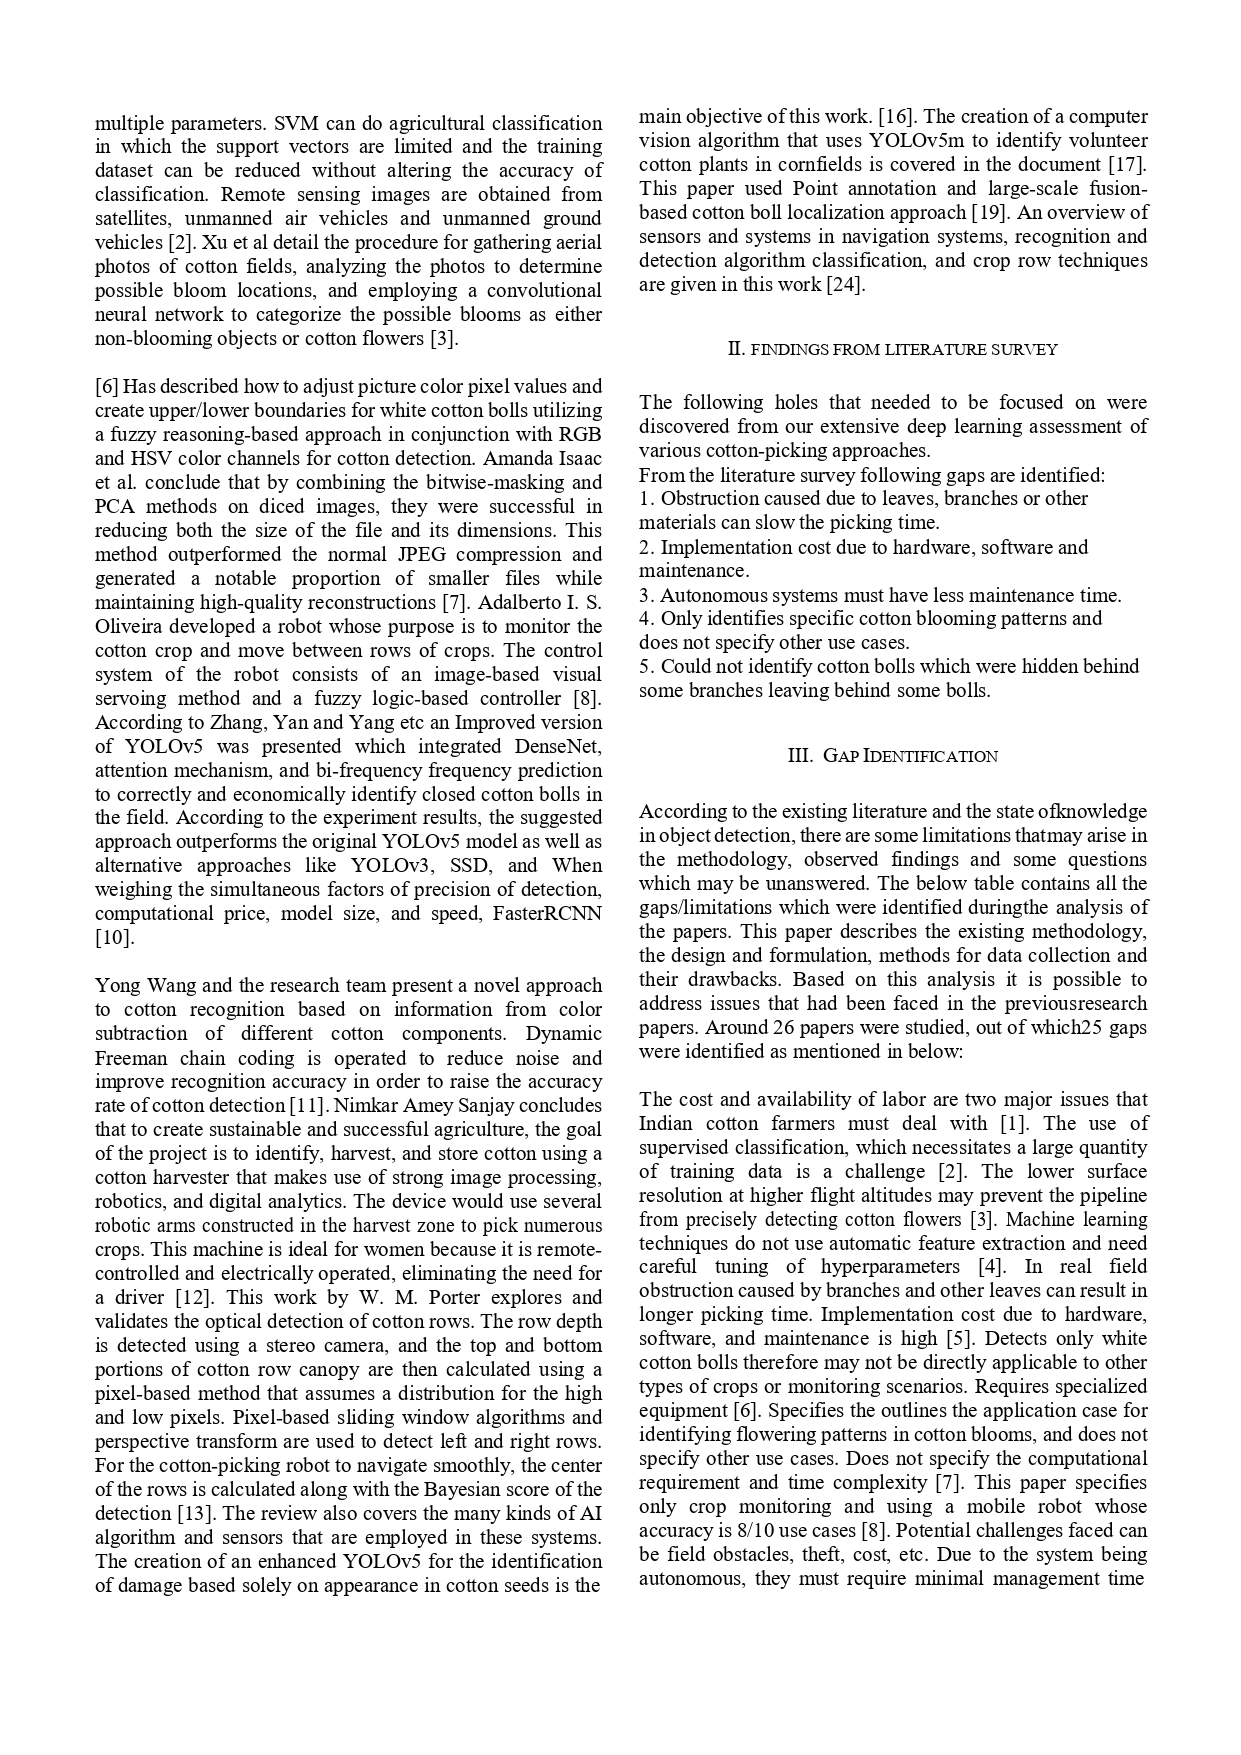
\includegraphics[scale=0.7]{images/copyright/publication/Publication/Publication_page-0002.jpg}
\newpage
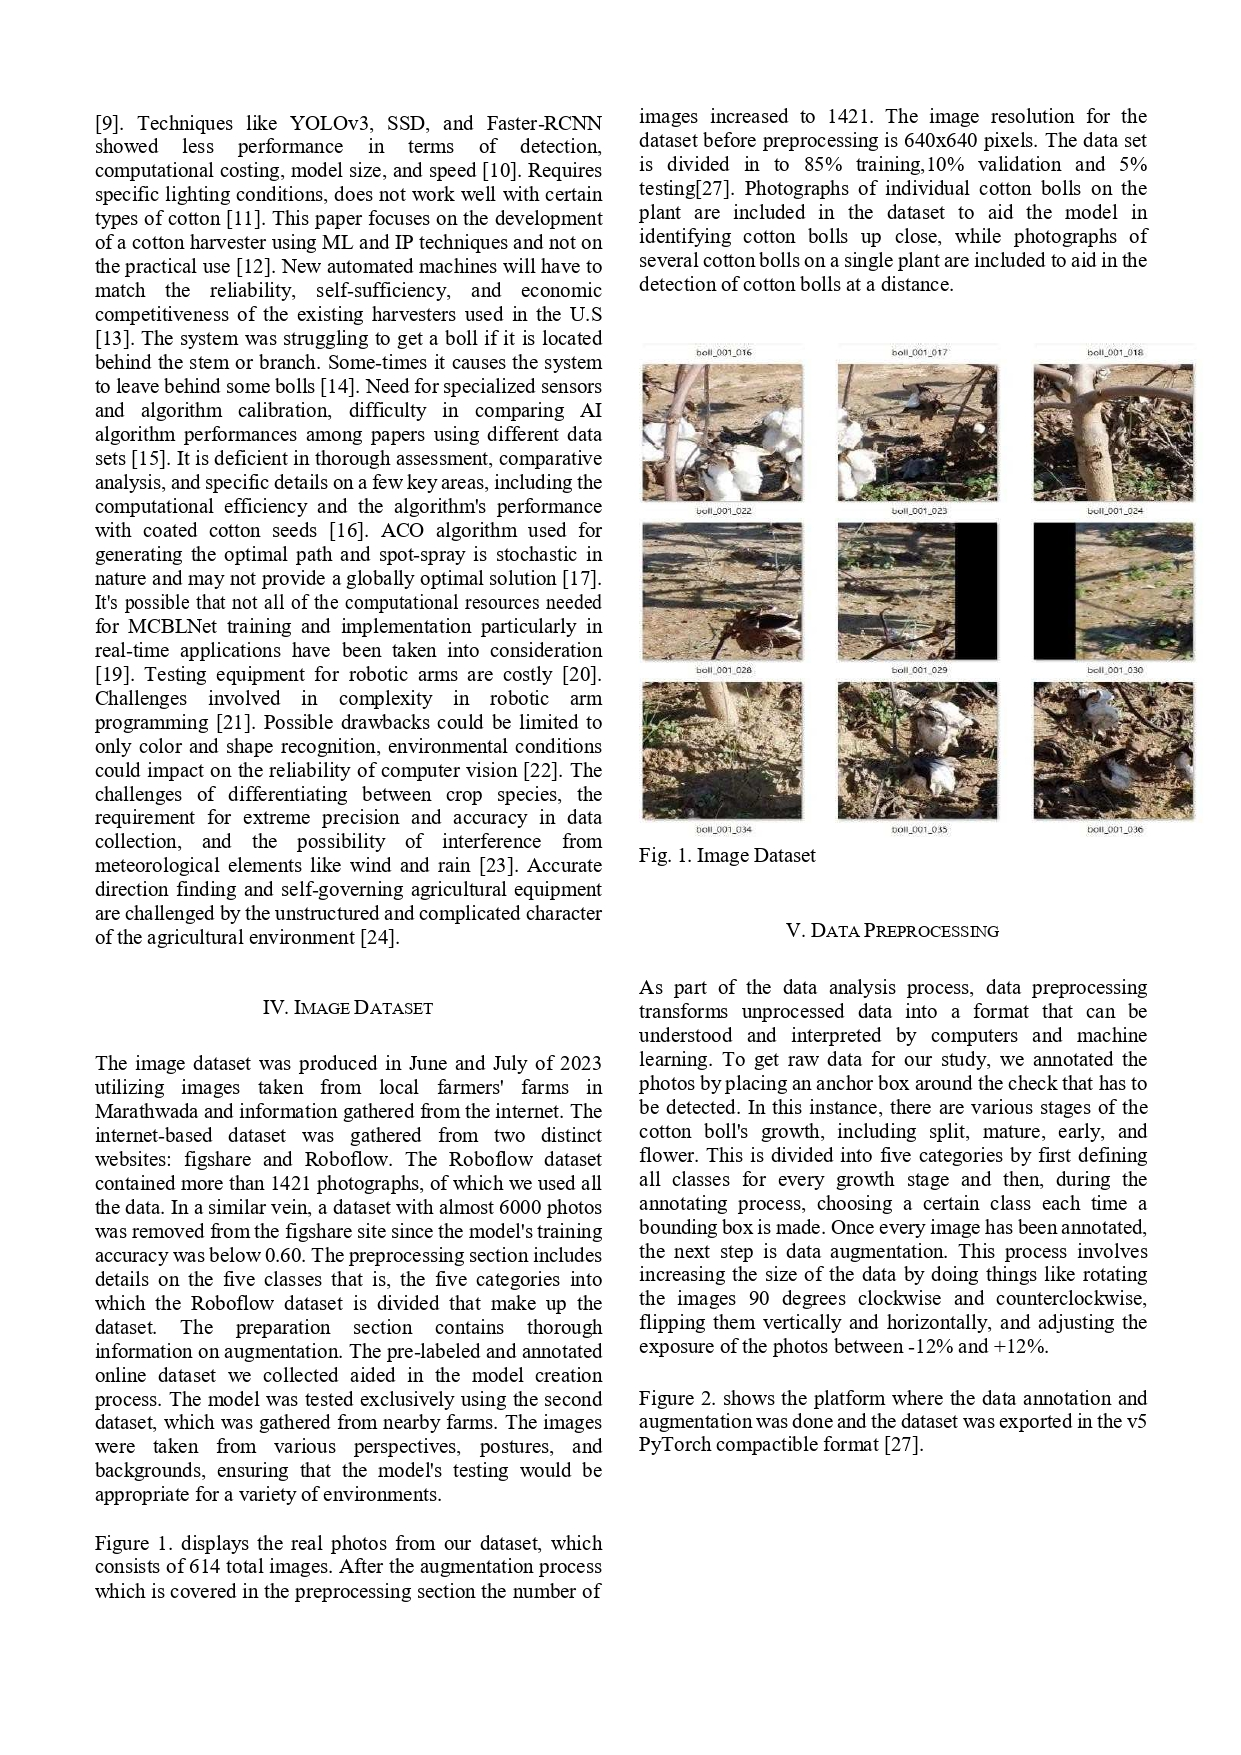
\includegraphics[scale =0.7]{images/copyright/publication/Publication/Publication_page-0003.jpg}
\newpage
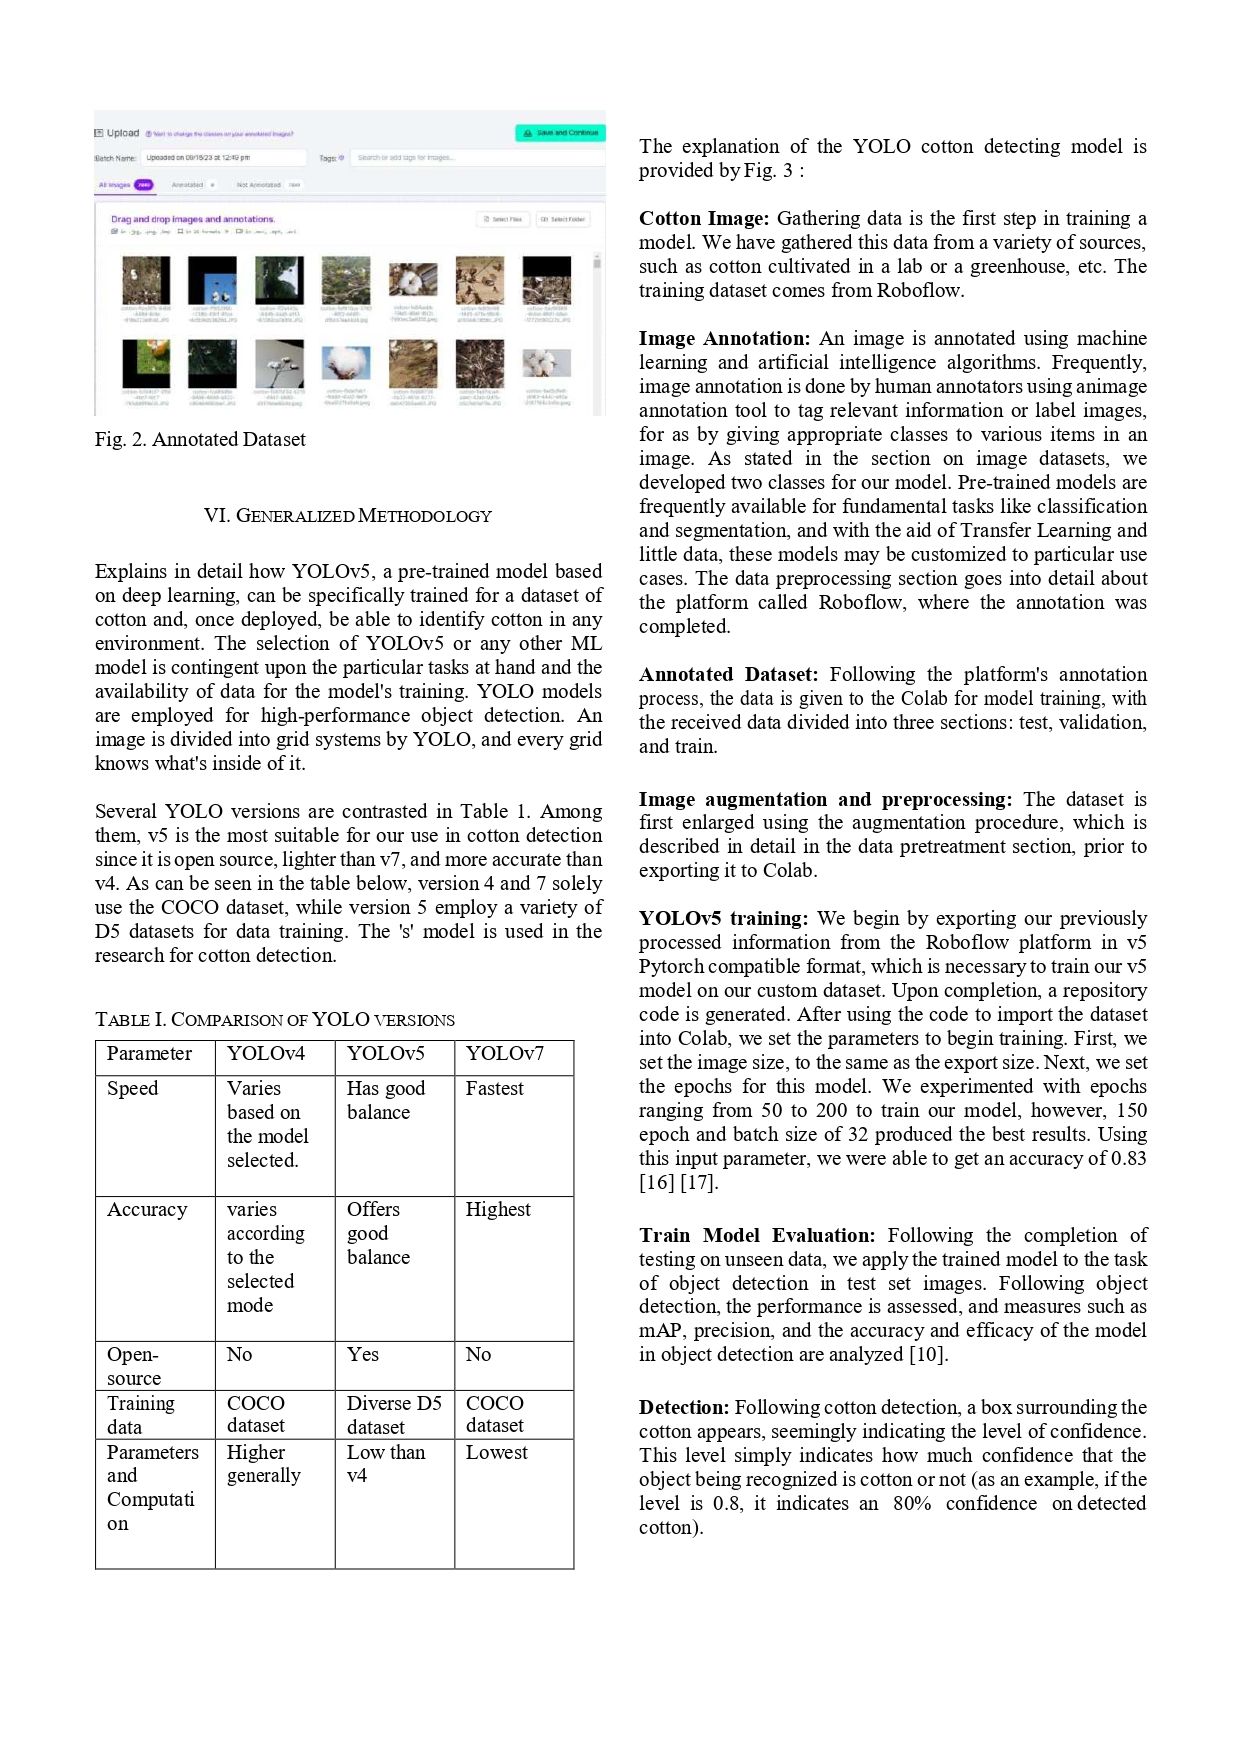
\includegraphics[scale=0.7]{images/copyright/publication/Publication/Publication_page-0004.jpg}
\newpage
\includegraphics[scale=0.7]{images/copyright/publication/Publication/Publication_page-0005.jpg}
\newpage
\includegraphics[scale=0.7]{images/copyright/publication/Publication/Publication_page-0006.jpg}
\newpage
\includegraphics[scale=0.7]{images/copyright/publication/Publication/Publication_page-0007.jpg}
\newpage

\subsection {Publication Copyright}
\includegraphics[scale =0.7]{images/copyright/publication/PublicationCopyright/PublicationCopyright_page-0001.jpg}
\newpage
\includegraphics[scale=0.7]{images/copyright/publication/PublicationCopyright/PublicationCopyright_page-0002.jpg}
\newpage
\includegraphics[scale =0.7]{images/copyright/publication/PublicationCopyright/PublicationCopyright_page-0003.jpg}
\newpage


\subsection {Publication Certificate}

\begin{figure}[!htb]
\begin{center}
\includegraphics[scale=0.5]{images/certificates/certificates/1477_Abhimanyu Rajesh Kanase_page-0001.jpg}
\end{center}
\end{figure}
\begin{figure}[!htb]
\begin{center}
\includegraphics[scale=0.5]{images/certificates/certificates/1477_Aditya Prasad Deshmukh-1_page-0001.jpg}
\end{center}
\end{figure} 
\begin{figure}[!htb]
\begin{center}
\includegraphics[scale=0.5]{images/certificates/certificates/1477_Anshu Biju Varghese_page-0001.jpg}
\end{center}
\end{figure} 







\section {Patent Documents}
\subsection {Patent Draft}
\includegraphics[scale =0.7]{images/patent/patent_doc/output-0000.jpg}
\newpage
\includegraphics[scale =0.7]{images/patent/patent_doc/output-0001.jpg}
\newpage
\includegraphics[scale =0.7]{images/patent/patent_doc/output-0002.jpg}
\newpage
\includegraphics[scale =0.7]{images/patent/patent_doc/output-0003.jpg}
\newpage
\includegraphics[scale =0.7]{images/patent/patent_doc/output-0004.jpg}
\newpage
\includegraphics[scale =0.7]{images/patent/patent_doc/output-0005.jpg}
\newpage
\includegraphics[scale =0.7]{images/patent/patent_doc/output-0006.jpg}
\newpage
\includegraphics[scale =0.7]{images/patent/patent_doc/output-0007.jpg}


\subsection {Patent}
\includegraphics[scale =0.4]{images/patent/patent_doc/patent.jpeg}

\newpage
\section {Copyright Certificate and Work Uploaded}
\subsection{Copyright Certificate}
\includegraphics[scale =0.6]{images/copyright/copyright_certificate/copyright_certificate_page-0001.jpg}
\newpage
\includegraphics[scale=0.7]{images/copyright/copyright_certificate/copyright_certificate_page-0002.jpg}
\newpage

\subsection{Synopsis}
\includegraphics[scale =0.7]{images/copyright/synopsis_new/Synopsis_new_page-0001.jpg}
\newpage
\includegraphics[scale=0.7]
{images/copyright/synopsis_new/Synopsis_new_page-0002.jpg}
\newpage
\includegraphics[scale=0.7]
{images/copyright/synopsis_new/Synopsis_new_page-0003.jpg}
\newpage
\includegraphics[scale=0.7]
{images/copyright/synopsis_new/Synopsis_new_page-0004.jpg}
\newpage
\includegraphics[scale=0.7]
{images/copyright/synopsis_new/Synopsis_new_page-0005.jpg}
\newpage

\subsection{Form 14}
\includegraphics[scale =0.7]
{images/copyright/Form14_page-0001.jpg}
\newpage
\includegraphics[scale=0.7]
{images/copyright/Form14_page-0002.jpg}
\newpage
\includegraphics[scale=0.7]
{images/copyright/Form14_page-0003.jpg}
\newpage
\includegraphics[scale =0.7]{images/copyright/Form14_page-0004.jpg}
\newpage
\includegraphics[scale =0.7]{images/copyright/Form14_page-0005.jpg }
\newpage


\end{document}




